\documentclass[11pt]{article}

% all packages used by any paper must be listed here
\usepackage{debulletin,times,epsfig,subfigure,wrapfig,algorithmic,color,boxedminipage,graphicx,url}

\usepackage{makecell}
\usepackage{multirow}
\usepackage{booktabs}
\usepackage{amsfonts}
\usepackage{amsmath,epsfig}
\usepackage{graphicx}
\usepackage{subfigure}
\usepackage{balance}
\usepackage{xspace,colortbl,subfigure,multirow}
\usepackage{mathrsfs}
\usepackage{amsmath}
\usepackage{cancel}
\usepackage{array}
\usepackage{verbatim}
\usepackage{bbm}
\usepackage{bm}
\usepackage{amsfonts}
\usepackage{color}
\usepackage{eurosym}
\usepackage{setspace,lipsum}
\usepackage{amsmath,amsfonts}
\usepackage{authblk}
%\usepackage{subfig}
\usepackage{url}
\usepackage{multirow}
\usepackage{paralist}
\usepackage{mathtools}
\usepackage{listings}
\usepackage{soul}
\usepackage{enumitem}
\usepackage{fancyvrb}





%\usepackage{algorithm,algorithmicx,algpseudocode} 

%\usepackage[font=small,labelfont=bf]{caption}


\begin{document}

% you may want to put in real date, vol no, issue no- but that is not necessary
\bulletindate{December 2018}
\bulletinvolume{41}
\bulletinnumber{4}
\bulletinyear{2018}

% these are files that I have- but your part of the issue can be done without
% them
\IEEElogo{cs.pdf}
\insidefrontcover{incvA18.pdf}
% \insidebackcover[TCDE Membership Form]{./calls/joinTCDE16.ps}

\begin{bulletin}

%
%  Letters to the editor section.  Use the lettersection environment.
%  Each letter is contained in a letter environment, where the two required
%  options to \begin{letter} are the author and the address of the author.
%

\begin{lettersection}

% there will be other letters- and a blank page will appear in your document
% but the special issue part will be fine

\begin{letter}{Farewell}
{David Lomet}{Microsoft Corporation}
\documentclass[11pt]{article} 

\usepackage{deauthor,times,graphicx}
%\usepackage{url}
\usepackage{hyperref}

\begin{document}


%\section*{Farewell}

It was way back in 1992 that Rakesh Agrawal, then the TCDE Chair, appointed me as Editor-in-Chief of the Data Engineering Bulletin. At the time, I saw it as a great opportunity. But it did not occur to me that it would become such an enormous part of my career. Now, 26 years later, it is time, perhaps past time, for me to pass this position on to younger hands, in this case to the capable hands of Haixun Wang. It should not come as a surprise that I am stepping down. Rather, the surprise should be ``why did I stay so long?'' This message is a combination of answer to that question and historical sketch of my time as EIC. These are not unrelated.

When I first became EIC, the Bulletin had already established a reputation as an industry and engineering focused publication, each issue of which was on a special topic.  Won Kim, my predecessor, had very capably established that publication model. Papers are solicited by each issue editor, with the editor selecting which authors to invite. The papers are a mix of work in progress, position statements, surveys, etc. But all focused on the special topic. I was determined not to screw this up. Indeed, I accepted the EIC appointment because I believed that the role that the Bulletin played is unique in our database community.  I stayed so long because I still believe that.  

Over the years, the Bulletin went through several major changes. As early as 1993, the Bulletin could be accessed online as well as via print subscription. This was a major transition. Mark Tuttle, then a colleague of mine in Digital (DEC) Cambridge Research Lab designed the latex style files that enabled this. Shortly thereafter, to economize on costs, the Bulletin became one of the earliest all electronic publications in our field. 

In 1995, hosting the Bulletin web site was provided by Microsoft- continuing until three years ago. Around 2010, the IEEE Computer Society became the primary host for the Bulletin. Around 2000, at the suggestion (prodding) of Toby Lehman,individual articles in addition to complete issues were served from the Bulletin web sites. Over this time, the style files and my procedures for generating the Bulletin evolved as well. Mark Tuttle again, and S. Sudarshan, who had been a Bulletin editor, provided help in evolving procedures used to generate the Bulletin and its individual articles. 

The Computer Society, and specifically staff members John Daniel, Carrie Clark Walsh, and Brookes Little, provided a TCDE email membership list used to distribute issue announcements, as well as helping in myriad other ways. The existence of dbworld (one of Raghu Ramakrishnan enduring contributions) enabled wider announcement distribution to our database community. The cooperation of Michael Ley with the prompt indexing of the Bulletin at dblp both ensured wider readership and provided an incentive for authors to contribute. Over the years, I was given great support by TCDE Chairs, starting with Rakesh Agrawal, then Betty Salzberg, Erich Neuhold, Paul Larson, Kyu-Young Whang, and Xiaofang Zhou. 

The most important part of being Bulletin EIC was the chance to work with truly distinguished members of the database community. It was enormously gratifying to have stars of our field (including eight Codd Award winners- so far) serving as editors. I take pride in appointing several of them as editors prior to their wider recognition.  It is the editors that deserve the credit for producing, over the years, a treasure trove of special issues on technologies that are central to our data engineering field. Superlative editors, and their success in recruiting outstanding authors, is the most important part of the Bulletin's success. Successfully convincing them to serve as editors is my greatest source of pride in the role I played as Bulletin EIC.  

Now I am happy to welcome Haixun to this wonderful opportunity.  Haixun's background includes outstanding successes in both research and industry.  He recently served ably as a Bulletin associate editor for issues on ``Text, Knowledge and Database'' and ``Graph Data Processing''.  His background and prior editorial experience will serve our data engineering community well and ensure the ongoing success of the Bulletin.  I wish him and the Bulletin all the best.

And so ``farewell''.  I will always treasure having served as Bulletin EIC for so many years. It was a rare privilege that few are given. Knowing that we were reaching you with articles that you found valuable is what has made the effort so rewarding to me personally. Thank you all for being loyal readers of the Bulletin. 

\end{document}


\end{letter}
\newpage
\begin{letter}{Letter from the Editor-in-Chief}
{Haixun Wang}{WeWork Corporation}
\documentclass[11pt]{article} 

\usepackage{deauthor,times,graphicx}
%\usepackage{url}
\usepackage{hyperref}

\begin{document}


\section*{Thank You, David!}

I know I represent the readers, the associate editors, and also the
broad database community when I say we are extremely grateful to David
Lomet for his distinguished and dedicated service as the
Editor-in-Chief of the Data Engineering Bulletin for the last 26
years.

Since its launch in 1977, the Bulletin has produced a total of 154
issues. Reading through the topics of the past issues that spanned
more than four decades makes me feel nothing short of amazing. They
show not just how far the database research has come, but to a certain
extent, how much the entire field of computer science and the IT
industry have evolved. While important topics never fail to arise in
the Bulletin in a timely fashion, it is also interesting to observe in
the 154 issues many recurring topics, including query optimization,
spatial and temporal data management, data integration, etc. It proves
that the database research has a solid foundation that supports many
new applications, and at the same time, it demonstrates that the
database research is constantly reinventing itself to meet the
challenges of the time. What the Bulletin has faithfully documented
over the last 42 years is nothing else but this amazing effort.

Among the 154 issues since the launch of the Bulletin, David had been
the Editor-in-Chief for 103 of them. This itself is a phenomenal
record worth an extra-special celebration. But more importantly, David
shaped the discussions and the topics in the long history of the
Bulletin.  I had the honor to work with David in 2016 and 2017 when I
served as the associate editor for two Bulletin issues. What was most
appealing to me was the opportunity of working with the top experts on
a topic that I am passionate about. The Bulletin is truly unique in
this aspect.

I understand the responsibility and the expectation of the
Editor-in-Chief, especially after David set such a great example in
the last 26 years. I thank David and the associate editors for their
trust, and I look forward to working with authors, readers, and the
database community on the future issues of the Data Engineering
Bulletin.

%\begin{flushright}
%Haixun Wang\\
%WeWork
%\end{flushright}
\end{document}


\end{letter}
%
\newpage
%
%% your introductory letter goes here
%

\begin{letter}{Letter from the Special Issue Editor}
{Joseph E. Gonzalez}{University of California at Berkeley\\ Berkeley, CA}
\graphicspath{{letters/}}
\documentclass[11pt]{article} 

\usepackage{deauthor,times,graphicx}
%\usepackage{url}
\usepackage{hyperref}



\begin{document}

Machine learning is rapidly maturing into an engineering discipline at the center of a growing range of applications.
This widespread adoption of machine learning techniques presents new challenges around the management of the data, code, models, and their relationship throughout the machine learning life-cycle.
In this special issue, 
% of the Data Engineering Bulletin 
we have solicited work from both academic and industrial leaders 
% in the data engineering community that 
who are exploring how data engineering techniques can be used to address the challenges of the machine learning life-cycle.




\begin{figure}[h]
\centering
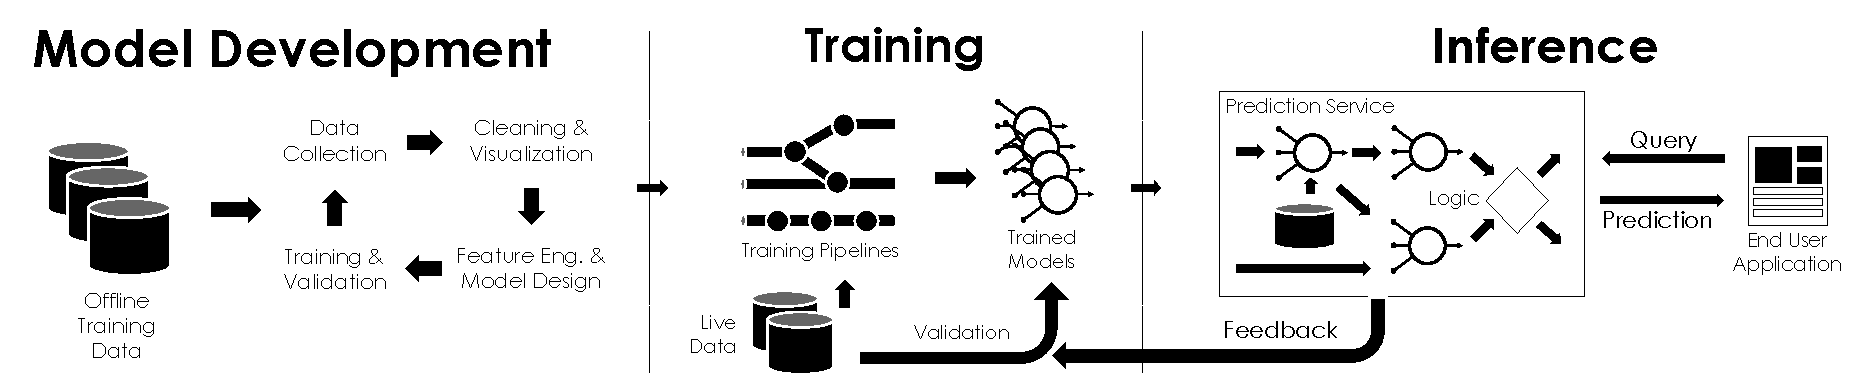
\includegraphics[width=\textwidth]{letters/pipeline.pdf}
\caption{\small \textbf{Machine Learning Life-cycle.} A simplified depiction of the key stages of a machine learning application.}
\label{fig:mllc}
\end{figure}


The machine learning life-cycle (Fig.~\ref{fig:mllc}) spans not only the model development but also production training and inference.
Each stage demands different skills (e.g., neural network design, data management, and cluster management) and imposes different requirements on the underlying systems.
Yet there is an overwhelming need for unifying design principles and technologies to address pervasive problems including feature management, data provenance, pipeline reproducibility, low-latency serving, and prediction monitoring just to name a few.


There has been a flurry of recent progress in systems to aid in managing the machine learning life-cycle.  
Large industrial projects like 
FB Learner Flow 
% \href{https://code.fb.com/core-data/introducing-fblearner-flow-facebook-s-ai-backbone/}{FB Learner Flow}
from Facebook, 
Michelangelo 
% \href{https://eng.uber.com/michelangelo/}{Michelangelo} 
from Uber, and 
TFX 
% \href{https://www.tensorflow.org/tfx/}{TFX} 
from Google have received considerable recent attention.  
In this issue, we have solicited papers from several recent industrial and academic projects that have received slightly less attention.


The first paper provides an overview of several real-world use cases and then outlines the key conceptual, data management, and engineering challenges faced in production machine learning systems.
% Rather than advocating a single system, this work describes some design principles that can inform potential solutions.
The second and third papers explores the challenges of model management and provenance across the machine learning life-cycle.
They motivate the need for systems to track models and their meta-data to improve reproducibility, collaboration, and governance. 
% expands upon the machine learning life-cycle 
% to include: data preparation, feature engineering, model training, deployment, and maintenance
% and explores the challenges of model 
The second paper introduces, ModelDB, an open-source system for model management and describe some of the functionality and design decisions. 
The third paper describes a related system, ProvDB, that uses a graph data model to capture and query fine-grained versioned lineage of data, scripts, and artifacts throughout the data analysis process.
The fourth paper describes, MLFlow, a new open-source system to address the challenges of experimentation, reproducibility, and deployment. 
This work leverages containerization to capture the model development environment and a simple tracking API to enable experiment tracking.
% The extensible model containerization enables model developers to more easily collaborate around modeling environments and then deploy model containers.
The fifth paper focuses on inference and explores the challenges and opportunities of serving white-box prediction pipelines.  
Finally, we solicited a summary of the recent Common Modeling Infrastructure (CMI) workshop at KDD 2018, which provides a summary of the keynotes and contributed talks.

The work covered here is only a small sample of the emerging space of machine learning life-cycle management systems. 
We anticipate that this will be a growing area of interest for the data engineering community.


% In contrast to the containerization of pipelines in MLFlow, the Microsoft team leverage knowledge about the internal of the prediction pipeline to more efficient serve predictions. 



\end{document}



\end{letter}

\end{lettersection}



% put the name of your special issue below
\begin{articlesection}{Machine Learning Life-cycle Management}
%
%  Contributed articles section.  Use the articlesection environment.
%  Each article is contained in an article environment, where the two required
%  options to \begin{article} are the title and author of the article
%
%\begin{article}
%{Title of article}
%{list of authors}
%\input{author-name/article.tex}
%\end{article}
\begin{article}
{On Challenges in Machine Learning Model Management}
{Sebastian Schelter, Felix Biessmann, Tim Januschowski, David Salinas, Stephan Seufert, Gyuri Szarvas}
\graphicspath{{submissions/adaptivedb/}}
%\documentclass[11pt,dvipdfm]{article}
\documentclass[11pt]{article}
\usepackage{deauthor,times,graphicx} %required
\usepackage{amsmath,amssymb}
\usepackage{multirow}
\usepackage{algorithm}
\usepackage{algpseudocode}
\usepackage{todonotes}
\usepackage{url}

% \graphicspath{{farnadi/}}

\newtheorem{mydef}{\textbf{Definition}}
\newtheorem{myex}{\textbf{Example}}
\newtheorem{mytheorem}{\textbf{Theorem}}


\begin{document}

\title{A Declarative Approach to Fairness in Relational Domains}
\author{Golnoosh Farnadi$^{1,2}$, Behrouz Babaki$^1$, Lise Getoor$^3$\\
$^1$Polytechnique Montr\'{e}al, $^2$ Mila, $^3$ UC Santa Cruz \\
farnadig@mila.quebec, behrouz.babaki@polymtl.ca, getoor@soe.ucsc.edu}

\maketitle

\begin{abstract}
AI and machine learning tools are being used with increasing frequency for decision making in domains that affect peoples' lives such as employment, education, policing and %loan approval
financial qualifications. These uses raise concerns about biases of algorithmic discrimination and have motivated the development of fairness-aware machine learning. However, existing fairness approaches are based solely on attributes of individuals. In many cases, discrimination is much more complex, and taking into account the social, organizational, and other connections between individuals is important. We introduce new notions of fairness that are able to capture the relational structure in a domain. We use first-order logic to provide a flexible and expressive language for specifying complex relational patterns of discrimination. Furthermore, we extend an existing statistical relational learning framework, probabilistic soft logic~(PSL), to incorporate our definition of relational fairness. We refer to this fairness-aware framework FairPSL. FairPSL makes use of the logical definitions of fairnesss but also supports a probabilistic interpretation. In particular, we show how to perform maximum a posteriori~(MAP) inference by exploiting probabilistic dependencies within the domain while avoiding violations of fairness guarantees. Preliminary empirical evaluation shows that we are able to make both accurate and fair decisions.
\end{abstract}

\section{Introduction}
\label{sec:introduction}

Over the past few years, AI and machine learning have become essential components in operations that drive the modern society, e.g., in financial, administrative, and educational spheres. \emph{Discrimination} happens when qualities of individuals which are not relevant to the decision making process influence the decision. Delegating decision making to an automated process raises questions about discriminating against individuals with certain traits based on biases in the data. This is especially important when the decisions have the potential to impact the lives of individuals, for example, the decisions on granting loans, assigning credit, and employment. 

\emph{Fairness} is defined as the absence of discrimination in a decision making process. The goal of \emph{fairness-aware} machine learning is to ensure that the decisions made by an algorithm do not discriminate against a population of individuals~\cite{feldman2015certifying2,boyd2014networked,hardt2016equality3}. Fairness has been well studied in the social sciences and legal scholarship (for an in-depth review see~\cite{barocas2016big2}), and there is emerging work on fairness-aware ML within the AI and computer science communities. For example, fairness through awareness/Lipschitz property~\cite{dwork2012fairness3}, individual fairness~\cite{zemel2013learning}, statistical parity/group fairness~\cite{kamishima2011fairness}, counterfactual fairness~\cite{counterfactualfairness}, demographic parity/disparate impact~\cite{feldman2015certifying2,chouldechova2017fair2}, preference-based fairness~\cite{zafar2017parity}, and equality of opportunity~\cite{hardt2016equality3}.

The existing work in fairness-aware machine learning is based on a definition of discrimination where a decision is influenced by an \emph{attribute} of an individual. An attribute value upon which discrimination is based (such as gender, race, or religion) is called a \emph{sensitive attribute}. The sensitive attribute defines a population of vulnerable individuals known as the \emph{protected group}. A fair decision-making process treats the protected group the same as the \emph{unprotected group}. 

However, in many social contexts, discrimination is the result of complex interactions and can not be described solely in terms of attributes of an individual. For example, consider an imaginary scenario in an organization in which younger female workers who have older male supervisors have lower chances of promotion than their male counterparts.\footnote{Of course, many other patterns may be possible: female bosses may promote female subordinates and discriminate against male workers, or male bosses may promote female employees.  Our goal is to provide a general framework which is able to describe arbitrarily complex discrimination patterns.} 
 This discrimination pattern involves two attributes of the individual (gender and age), a relationship with another individual (supervisor), and two attributes of the second individual. Addressing such complex cases poses two challenges. First, the concepts of discrimination and fairness need to be extended to capture not only attributes of individuals but also the relationships between them. Second, a process is required that ensures that fair decisions are made about individuals who are affected by such patterns. In this paper we address both of these challenges.
We use first-order logic (FOL) to extend the notion of fairness to the relational setting. FOL is an expressive representation for relational problems which is also widely used for learning in relational domains. Moreover, we extend an existing framework for statistical relational learning~\cite{getoor2007introduction} called probabilistic soft logic (PSL)\footnote{http://psl.linqs.org/}~\cite{bach:jmlr17}. PSL combines logic and probability for learning and reasoning over uncertain relational domains. One of the most common reasoning tasks in PSL is called maximum a posteriori (MAP) inference, which is performed by finding the most probable truth values for unknowns over a set of given evidence. We develop a new MAP inference algorithm which is able to maximize the a posteriori values of unknown variables \emph{subject to} fairness guarantees. An early version of this paper which this work builds upon and extends appeared in~\cite{farnadi2018fairness}.

\looseness-1
Our contributions are as follows: 1) we propose fairness-aware machine learning for the relational setting; 2) we extend PSL into a fairness-aware framework called FairPSL which can represent the logical definition of fairness; 3) we develop a new MAP inference algorithm which is able to maximize the posteriori values of unknown variables \emph{subject to} fairness guarantees; 4) we empirically evaluate our proposed framework on synthetic data. 

\section{Motivation}
\label{sec:motivation}

Discrimination in social contexts have been studied in the field of social psychology~\cite{brewer2007social,brewer1979group,ridgeway2004unpacking}. There is a large literature on various aspects of relational bias in social contexts such as \emph{in-group-out-group bias}, \emph{gender bias}, and \emph{ethnicity-based favoritism} that can result in discrimination. 
As an example, consider gender bias in the workplace that reflects stereotypically masculine criteria and male-based favoritism. Such gender bias 
typically places women in lower positions and negatively impacts their opportunities. Further, lack of women in leadership positions may affect the promotion of women and results in a glass ceiling that keeps women from rising beyond a certain level in the hierarchy. This scenario shows that considering  protected attributes such as gender is not always sufficient to detect the source of bias and avoid discrimination, one also has to consider the relational information, in this case the organization hierarchy. Note that this can be generalized to any ingroup/outgroup scenario where the sensitive attribute could be race, religion, age, marital-status, etc.

The existing work on designing fair algorithms in machine learning exclusively focuses on \emph{attribute-based fairness}, which is based on the following assumptions: First, there is an assumption that the individuals (sometimes referred to as units or entities) are independent and described by simple attribute vectors. Second, the group for which one wishes to ensure fairness (known as the \emph{protected group}) is defined on the basis of some attribute values. Finally, there is a decision that is associated with each individual, and the goal is to ensure that members of the protected group are subject to a fair decision (we discuss different fairness measures in Section~\ref{sec:fairnessmeasure}).  We illustrate  attribute-based fairness in the following example. 

\begin{myex}[Loan Processing]
\label{ex:loan}
A bank bases its decisions about granting a loan on attributes of the applicant. The goal is to decide whether to grant a loan to an applicant using a predictive model. The bank needs to ensure that the obey fair lending practices and ensure that gender, race, sexual orientation of applicants has no influence on the decision. In this scenario, the protected group is the historically disadvantaged applicants.  
\end{myex}
The current fairness-aware machine learning techniques are not capable of modeling relations and hence cannot be used to make the decision making model fair. However, in many decision making scenarios, especially in social and organizational settings, the domain is relational, and the protected group itself might be best represented using a relational definition. We illustrate this setting in the following scenario:
\begin{myex}[Performance Review]
\label{ex:review}
Consider an organization where decisions about the promotion of employees is based on two criteria: 1) an objective performance measure, and 2) the opinion of their direct and indirect managers above them. The opinions are inferred from the performance reviews which are collected periodically. Not every manager can submit a review for all its subordinates, this is especially the case for top-level managers who have a large number of subordinates. Hence, the opinions of managers are collectively inferred from the opinions of their sub-ordinates. However, some employees may be biased, and judge other employees unfavorably, by favoring employees who are similar to themselves (same gender, race, religion, etc.) over employees who are dissimilar. The organization needs to ensure that promotion of employees do not have any relational bias caused by in-group-out-group favoritism.

\end{myex}
Example~\ref{ex:review} describes a prediction problem over a database that consists of relations between employees. Such prediction tasks are best handled by techniques from the relational learning domain. To ensure fair prediction in such settings, we need to extend the notion of \emph{attribute-based fairness} to \emph{relational fairness}. Throughout this paper, we use the performance review problem as a running example for relational fairness.

\section{Fairness Formalism}
\label{sec:formulation}

A representation that can describe different types of entities and different relationships between them is called relational. In this section, we use first-order logic to define relational fairness. We employ first-order logic as an expressive representation formalism which can represent objects and complex relationships between them. We start by defining an atom:

\begin{mydef}[Atom]
An atom is an expression of the form $P(a_1, a_2, \ldots, a_n)$ where each argument $a_1, a_2,$ $\ldots,$ $a_n$ is either a constant or a variable. The finite set of all possible substitutions of a variable to a constant for a particular variable $a$ is called its \textit{domain} $D_{a}$. If all variables in $P(a_1, a_2, \ldots, a_n)$ are substituted by some constant from their respective domain, then we call the resulting atom a \textit{ground atom}. 
\end{mydef}

\begin{myex}
In our loan processing problem (Example~\ref{ex:loan}), we can represent applicants' attributes by atoms. For instance, atom $Female(v)$ indicates whether or not applicant $v$ is female. Similarly, we can represent relations with atoms. In the performance review problem in Example~\ref{ex:review} the atom $Manager(m,e)$ indicates whether or not employee $m$ is a direct or indirect manager of employee $e$.
\end{myex}

The relational setting provides the flexibility to express complex definitions with formulae.

\begin{mydef}[Formula] 
A formula is defined by induction: every atom is a formula. If $\alpha$ and $\beta$ are formulae, then $\alpha \vee \beta$, $\alpha \wedge \beta$, $\neg \alpha$, $\alpha \rightarrow \beta$ are formulae. If $x$ is a variable and $\alpha$ is a formula, then the quantified expressions of the form $\exists x$ $\alpha$ and $\forall x$ $\alpha$ are formulae.    
\end{mydef}

To characterize groups of individuals based on a formula, we define the notion of \emph{population}.

\begin{mydef}[Population]
We denote formula $F$ which has only one free variable $v$ (i.e., other variables in $F$ are quantified) by $F[v]$. The population defined by $F[v]$ is the set of substitutions of $v$ for which $F[v]$ holds.   
\end{mydef}


\begin{myex}
\label{ex:disformula}
Consider the formula $F[v] := \forall u, \, \textit{Manager}(u,v) \rightarrow \neg \textit{SameGroup}(u, v)$. The population specified by this formula is the set of individuals all of whose managers belong to a group different from theirs. 
\end{myex}

The truth value of a formula is derived from the truth value of atoms that it comprises, according to the rules of logic. Each possible assignment of truth values to ground atoms is called an \emph{interpretation}. 


\begin{mydef}[Interpretation]
An interpretation $I$ is a mapping that associates a truth value $I(P)$ to each ground atom $P$. For Boolean truth values, $I$ associates true to 1 and false to 0 truth values. For soft logic (see Definition~\ref{def:softlogic}) $I$ maps each ground atom $P$ to a truth value in interval $[0, 1]$.
\end{mydef}

In attribute-based fairness, it is assumed that there is a certain attribute of individuals, i.e, the sensitive attribute,  that we do not want to affect a decision. Gender, race, religion and marital status are examples of sensitive attributes. Discrimination has been defined in social science studies as a treatment in favor or against a group of individuals given their sensitive attribute. This group of individuals is the protected group. 

In a relational setting, both the sensitive attributes of an individual and their participation in various relations may have an undesired effect on the final decision. We characterize the protected group in a relational setting by means of a population. In practice, we are often interested in maintaining fairness for a specific population such as applicants, students, employees, etc. This population is then partitioned into the protected and unprotected groups. We define a \emph{discriminative pattern} which is a pair of formulae to capture these groups: 1) $F_1[v]$: to specify the difference between the protected and unprotected groups and 2) $F_2[v]$: to specify the population over which we want to maintain fairness. 

\begin{mydef}[Discriminative pattern]
A discriminative pattern is a pair $\textit{DP}[v]:=(F_1[v], F_2[v])$ , where $F_1[v]$ and $F_2[v]$ are formulae.
\end{mydef}

\begin{myex}
\label{ex:pattern}
The two formulae in the discrimination pattern $\textit{DP}[v]:= \big((\forall u, \,  \textit{Manager}(u,v) \rightarrow  \neg \textit{SameGroup}(u, v)),$ $\textit{Employee}(v)\big)$ specify two populations, namely all employees and those employees who belong to a group different from their managers.
\end{myex}

Given the definition of the discriminative pattern, we have a rich language to define the scope of the protected and unprotected groups in a relational setting.

\begin{mydef}[Protected group] Given an interpretation $I$, the protected group is a population of the form:
{$$PG :=\{ v : F_1[v] \wedge F_2[v]\}$$}
which is defined as the set of all instances hold for variable $v$ for which $F_1[v] \wedge F_2[v]$ is true under interpretation $I$, that is, $I(F_1[v] \wedge F_2[v]) = 1$. 
Similarly, the \emph{unprotected group} is a population of the form: 
{$$UG := \{ v : \neg F_1[v] \wedge  F_2[v]\}$$}
which is defined as the set of all instances hold for variable $v$ 
for which $I(\neg F_1[v] \wedge F_2[v]) = 1$. 
\end{mydef}

\begin{myex}
The protected group of the discrimination pattern specified in Example~\ref{ex:pattern} is {$PG := \big\{ v : \big(\forall u, \,$ $ \textit{Manager}(u, v) \rightarrow \neg \textit{SameGroup}(u, v)\big) \wedge \textit{Employee}(v) \big\}$} and the unprotected group is {$UG :=  \big\{ v:  \big(\exists u, \, \textit{Manager}(u,v) \wedge \textit{SameGroup}(u, v)\big) \wedge \textit{Employee}(v) \big\}$}. This means our protected group is the set of employees belonging to a group different from their managers,
and our unprotected group consists of other employees. 
\end{myex}

Discrimination is defined in terms of a treatment or decision that distinguishes between the protected and unprotected groups. Here we define the \emph{decision} atom.
\begin{mydef}[Decision atom] A decision atom $d(v)$ is an atom containing exactly one variable $v$ that specifies a decision affecting the protected group which is defined either by law or end-user.
\end{mydef}
\begin{myex}
The decision atom ${\textit ToPromote}(v)$ indicates whether or not $v$ receives a promotion.
\end{myex}

Note that the fairness formulation in this section is designed for the relational setting, however relational fairness subsumes the attribute-based fairness such that: a sensitive attribute is defined by an atom with one argument and $F_2[v]$ in discrimination pattern is $\textit{Applicant}(v)$. For example, discrimination pattern of our loan processing problem in Example~\ref{ex:loan} is of the form $\textit{DP} := ( \textit{Female}(v), \textit{Applicant}(v))$ that denotes female applicants as the protected group (i.e., $PG :=  \{ v: \textit{Female}(v) \}$) and male applicants as the unprotected group (i.e., $UG := \{ v: \neg \textit{Female}(v)\}$).


\section{Fairness Measures}
\label{sec:fairnessmeasure}

Over the past few years, many fairness measures have been introduced~\cite{verma2018fairness2}. An important class of these measures are \emph{group fairness} measures which quantify the inequality between different subgroups. Some of the most popular measures in this class include \emph{equal opportunity}, \emph{equalized odds}, and \emph{demographic parity}~\cite{hardt2016equality3}. In this paper we restrict our focus to the latter. In an attribute-value setting, demographic parity means that the decision should be independent of the protected attributes. Assume that binary variables $A$ and $C$ denote the decision and protected attributes, and the preferred value of $A$ is one. Demographic parity requires that:

\begin{equation*}
    P(A=1 | C=0) = P(A=1 | C=1)
\end{equation*}

We will now generalize this measure to the relational setting using the notations defined in Section~\ref{sec:formulation}. Let $a$ and $c$ denote the counts of denial (i.e., negative decisions) for protected and unprotected groups, and $n_{1}$ and $n_{2}$ denote their sizes, respectively. Given the decision atom $d(v)$, discriminative pattern $\textit{DP}(F_1[v], F_2[v])$, and interpretation $I$, these counts are computed by the following equations: 
{
\begin{flalign}
    & a \equiv \sum_{v \in D_v} I\big( \neg d(v) \wedge  F_1[v] \wedge F_2[v]) \label{eq:a}\\
    & c \equiv \sum_{v \in D_v} I\big( \neg d(v) \wedge  \neg F_1[v] \wedge  F_2[v]) \label{eq:c}\\
    & n_{1} \equiv \sum_{v \in D_v} I\big(F_1[v] \wedge F_2[v]) \label{eq:n1}\\
    & n_{2} \equiv \sum_{v \in D_v} I\big(\neg F_1[v] \wedge  F_2[v]) \label{eq:n2}
\end{flalign}}
The proportions of denying for protected and unprotected groups are $p_1 = \frac{a}{n_1}$ and $p_2 = \frac{c}{n_2}$, respectively. There are a number of data-driven measures~\cite{Pedreschi:2012} which quantify demographic disparity and can be defined in terms of $p_1$ and $p_2$:
\begin{itemize}
    \item \textbf{Risk difference}: $RD = p_1 - p_2$, also known as absolute risk reduction. 
    \item \textbf{Risk Ratio}: $RR = \frac{p_1}{p_2}$, also known as relative risk. 
    \item \textbf{Relative Chance}: $RC = \frac{1 - p_1}{1 - p_2}$ also, known as selection rate.
\end{itemize}
These measures have been used in the legal systems of European Union, UK, and US~\cite{EUlaw,UKlaw,USlaw}. Notice that RR is the ratio of the proportion of benefit denial between the protected and unprotected groups, while RC is the ratio of the proportion of benefit granted. Finally, we introduce the notion of $\delta$-fairness.

\begin{mydef}[$\delta$-fairness]
If a fairness measure for a decision making process falls within some $\delta$-window, then the process is \emph{$\delta\text{-fair}$}. Given $0 \leq \delta \leq 1$, the  $\delta$-windows for measures RD/RR/RC are defined as:
{\begin{flalign*}
	     - \delta \leq &RD \leq \delta \\
	     1- \delta \leq &RR \leq 1+ \delta\\
	     1- \delta \leq &RC \leq 1+ \delta
	\end{flalign*}}
\end{mydef}

To overcome the limitations of attribute-based fairness, we introduce a new statistical relational learning~(SRL) framework~\cite{getoor2007introduction} suitable for modelling fairness in relational domain. In the next section, we review probabilistic soft logic~(PSL). We then extend PSL with the definition of relational fairness introduced above in Section~\ref{sec:fairMAP}. Our fairness-aware framework, ``FairPSL'', is the first SRL framework that performs fair inference. 

\section{Background: Probabilistic Soft Logic}
\label{sec:psl}

In this section, we review the syntax and semantics of PSL, and in the next section we extend MAP inference in PSL with fairness constraints to define MAP inference in FairPSL.

PSL is a probabilistic programming language for defining hinge-loss Markov random fields~\cite{bach:jmlr17}. Unlike other SRL frameworks whose atoms are Boolean, atoms in PSL can take continuous values in the interval $[0,1]$. PSL is an expressive modeling language that can incorporate domain knowledge with first-order logical rules and has been used successfully in various domains, including bioinformatics~\cite{sridhar:bioinformatics16}, recommender systems~\cite{kouki:recsys15}, natural language processing~\cite{ebrahimi:emnlp16}, information retrieval~\cite{alshukaili:iswc16}, and social network analysis~\cite{west2014exploiting}, among many others. 
 
A PSL model is defined by a set of first-order logical rules called \emph{PSL rules}.

\begin{mydef} [PSL rule] a PSL rule $r$ is an expression of the form:
{\begin{equation}
\lambda_{r}: T_1 \land T_2 \land \ldots \land T_w \rightarrow H_1 \vee H_2 \vee \ldots \vee H_l
\end{equation}}

where { $T_1, T_2, \ldots, T_w, H_1, H_2, \ldots, H_l$} are atoms or negated atoms and { $\lambda_{r} \in \mathbb{R}^{+} \cup \infty$} is the weight of the rule $r$.  We call { $T_1 \land T_2 \land \ldots \land T_w$} the body of $r$ ($r_{body}$), and { $H_1 \vee H_2 \vee \ldots \vee H_l$} the head of $r$ ($r_{head}$).
\end{mydef}


Since atoms in PSL take on continuous values in the unit interval $[0,1]$, next we define soft logic to calculate the value of the PSL rules under an interpretation $I$.

\begin{mydef}[Soft logic]
\label{def:softlogic}
The ({$\tilde{\wedge}$}) and ({$\tilde{\vee}$}) and negation ({$\tilde{\neg}$}) are defined as follows. For {$m, n \in [0,1]$} we have: {$m \tilde{\wedge} n = \max(m+n -1, 0)$}, {$m \tilde{\vee} n = \min(m+n , 1)$} and {$\tilde{\neg} m = 1 - m$}. The $\, \tilde{} \,$ indicates the relaxation over Boolean values.
\end{mydef}

The probability of truth value assignments in PSL is determined by the rules' \emph{distance to satisfaction}.

\begin{mydef}[The distance to satisfaction]
The distance to satisfaction $d_{r}(I)$ of a rule $r$ under an interpretation $I$ is defined as:
{
\begin{equation}
d_{r}(I) = \max\{0, I(r_{body})-I(r_{head})\}
\end{equation}}
\end{mydef}

By using Definition~\ref{def:softlogic}, one can show that the closer the interpretation of a grounded rule $r$ is to 1, the smaller its distance to satisfaction. A PSL model induces a distribution over interpretations $I$. Let $R$ be the set of all grounded rules, then the probability density function is:
{
\begin{equation}
f(I) ={\frac{1}{Z}} \exp[-\sum_{r\in R} \lambda_{r}(d_{r}(I))^p]
\label{eq:potential}
\end{equation}
}
\noindent where { $\lambda_{r}$} is the weight of rule $r$, {
$Z = \int_{I} \exp[ -\sum_{r\in R} \lambda_{r}(d_{r}(I))^p]$
} is a normalization constant, and { $p \in \{1,2\}$} provides a choice of two different loss functions, $p=1$ (i.e., linear), and $p=2$ (i.e, quadratic). These probabilistic models are instances of hinge-loss Markov random fields~(HL-MRF)~\cite{bach:jmlr17}. The goal of maximum a posteriori (MAP) inference is to find the most probable truth assignments $I_{\textit{MPE}}$ of unknown ground atoms given the evidence which is defined by the interpretation $I$. Let $X$ be all the evidence, i.e., $X$ is the set of ground atoms such that $\forall x \in X, I(x)$ is known, and let $Y$ be the set of ground atoms such that $\forall y \in Y, I(y)$ is unknown. Then we have
{
\begin{equation}
I_{\textit{MAP}}(Y) = \textit{arg}\max_{I(Y)} P(I(Y)|I(X))
\end{equation}}
Maximizing the density function in Equation~\ref{eq:potential} is equivalent to minimizing the weighted sum of the distances to satisfaction of all rules in PSL. 

\begin{table*}[t]
    \centering
    \begin{tabular}{|lll|}
    \hline
    &&\\
    $R1$ & $\lambda_1$ &: $\textit{IsQualified}(e) \rightarrow \textit{HighPerformance}(e)$ \\
    $R2$ & $\lambda_1$ &: $\neg \textit{IsQualified}(e) \rightarrow \neg \textit{HighPerformance}(e)$ \\
    $R3$ & $\infty$ &: $\textit{PositiveReview}(e1, e2) \rightarrow \textit{PositiveOpinion}(e1, e2)$ \\
    $R4$ & $\infty$ &: $\neg \textit{PositiveReview}(e1, e2) \rightarrow \neg \textit{PositiveOpinion}(e1, e2)$ \\
    $R5$ & $\lambda_1$ &: $\textit{PositiveOpinion}(e1, e2) \wedge \textit{Manager}(m, e1) \rightarrow \textit{PositiveOpinion}(m, e2)$ \\
    $R6$ & $\lambda_1$ &: $\neg \textit{PositiveOpinion}(e1, e2) \wedge \textit{Manager}(m, e1) \rightarrow \neg \textit{PositiveOpinion}(m, e2)$ \\
    $R7$ & $\lambda_1$ &: $\textit{PositiveOpinion}(m, e) \wedge \textit{Manager}(m, e) \rightarrow \textit{IsQualified}(e)$ \\
    $R8$ & $\lambda_1$ &: $\neg \textit{PositiveOpinion}(m, e) \wedge \textit{Manager}(m, e) \rightarrow \neg \textit{IsQualified}(e)$ \\
    $R9$ &  $\lambda_1$ &: $\neg \textit{ToPromote}(e)$\\
    $R10$ & $\infty$ &: $\textit{IsQualified}(e) \rightarrow \textit{ToPromote}(e)$ \\
    $R11$ & $\infty$ &: $\neg \textit{IsQualified}(e) \rightarrow \neg \textit{ToPromote}(e)$ \\
    &&\\
    \hline
    \end{tabular}
    \caption{\small A simplified PSL model for the \emph{Performance Reviewing} problem}
    \label{tab:pslmodel}
\end{table*}

\begin{myex}
\label{ex:pslmodel}
The simplified PSL model for the performance reviewing problem in Example\ref{ex:review} is given in Table~\ref{tab:pslmodel}. The goal of MAP inference for this problem is to infer employees to promote. We simplified the model by assigning the same weight to all soft rules (i.e., $\lambda_i= 1$ where $i=\{1,2,5,6,7,8,9\}$). Below we explain the meaning of each rule in the model.

Rule $R1$ indicates that qualified employees have high performance and similarly rule $R2$ expresses that a negative qualification of employees is derived from their low performance. Rules $R5$ and $R6$ presents the propagation of opinion from bottom to top of the organizational hierarchy, i.e., managers have similar opinions towards employees given the opinions of their sub-ordinate managers. And rules $R7$ and $R8$ indicate that the positive/negative opinion of direct/indirect managers derive from the qualification of an employee. Rule $R9$ indicates the prior that not all employees get promoted. We also have four hard constraints (i.e., rules $R3$, $R4$, $R10$ and $R11$) where the weight of the rules are $\infty$. Rules $R3$ and $R4$ indicate that submitted positive/negative reviews should reflect positive/negative opinions. And two rules $R10$ and $R11$ show that a highly qualified employee should get promoted. 
\end{myex}

\section{Fairness-aware PSL (FairPSL)}
\label{sec:fairMAP}

The standard MAP inference in PSL aims at finding values that maximize the conditional probability of unknowns. Once a decision is made according to these values, one can use the fairness measure to quantify the degree of discrimination. A simple way to incorporate fairness in MAP inference is to add the $\delta$-fairness constraints to the corresponding optimization problem.   

Consider risk difference, $\textit{RD}$, where $\textit{RD} \equiv \frac{\mathbf{a}}{n_1} - \frac{\mathbf{c}}{n_2}$. The $\delta$-fairness constraint $-\delta \leq \textit{RD} \leq \delta$ can be encoded as the following constraints:
{\begin{align}
    & n_2 \mathbf{a} - n_1 \mathbf{c} - n_1 n_2 \delta \leq 0 \label{eq:RD1}\\
    & n_2 \mathbf{a} - n_1 \mathbf{c} + n_1 n_2 \delta \geq 0
\end{align}}
Similarly, from $\textit{RR} \equiv \frac{\mathbf{a} / n_1}{\mathbf{c} / n_2}$ and the $\delta$-fairness constraint $1 - \delta \leq \textit{RR} \leq 1 + \delta$ we obtain:
{\begin{align}
    & n_2 \mathbf{a} - (1 + \delta) n_1 \mathbf{c} \leq 0 \\
    & n_2 \mathbf{a} - (1 - \delta) n_1 \mathbf{c} \geq 0
\end{align}}
And finally, $\textit{RC} \equiv \frac{1 - \mathbf{a} / n_1}{1 - \mathbf{c} / n_2}$ and the $\delta$-fairness constraint $1 - \delta \leq \textit{RC} \leq 1 + \delta$ gives:
{ \begin{align}
    & - n_2 \mathbf{a} + (1 + \delta) n_1 \mathbf{c} - \delta n_1 n_2 \leq 0 \\
    & - n_2 \mathbf{a} + (1 - \delta) n_1 \mathbf{c} + \delta n_1 n_2 \geq 0 \label{eq:RC2}
\end{align}}
A primary advantage of PSL over similar frameworks is that its MAP inference task reduces to a convex optimization problem which can be solved in polynomial time. To preserve this advantage, we need to ensure that the problem will remain convex after the addition of $\delta$-fairness constraints. 

\begin{mytheorem}
The following condition is sufficient for preserving the convexity of MAP inference problem after addition of $\delta$-fairness constraints: The formulae $F_1[v]$ and $F_2[v]$ do not contain an atom $y \in Y$ and all atoms in $F_1[v]$ and $F_2[v]$ have values zero or one.
\end{mytheorem}
\begin{proof}
Since $I(F_1[v])$ and $I(F_2[v])$ do not depend on $I(Y)$, the values $n_{1}$ and $n_{2}$ are constants that can be computed in advance. Let us define the sets $D_v^a = \{ v \in D_v : F_1[v] \wedge F_2[v] \, \text{is true} \}$ and $D_v^c = \{ v \in D_v : \neg F_1[v] \wedge F_2[v] \, \text{is true} \}$. Since $F_1[v]$ and $F_2[v]$ can be only zero or one, we can rewrite the equations~\ref{eq:a} and \ref{eq:c} as:
{
\begin{align*}
    & \mathbf{a} = \sum_{v \in D_v^a} I(\neg d(v)) = |D_v^a| - \sum_{v \in D_v^a} I(d(v))\\
    & \mathbf{c} = \sum_{v \in D_v^c} I(\neg d(v)) = |D_v^c| - \sum_{v \in D_v^c} I(d(v))
\end{align*}}
\noindent which indicates that $\mathbf{a}$ and $\mathbf{c}$ can be expressed as linear combinations of variables in the optimization problem. This means that constraints~\ref{eq:RD1}-\ref{eq:RC2} are linear. Hence, addition of these constraints preserves the convexity of the optimization problem. 
\end{proof}

\section{Experiments}
\label{sec:experiment}

\begin{figure}
  \begin{minipage}[c]{0.6\textwidth}
    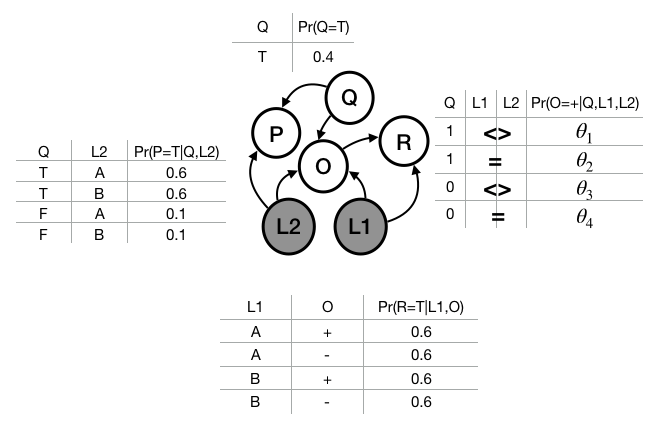
\includegraphics[width=\textwidth]{figs/BN.png}
  \end{minipage}\hfill
  \begin{minipage}[c]{0.45\textwidth}
    \caption{
        \small The model used for generating the datasets. There are four binary random variables, P, Q, O, and R. \textbf{P}: indicates whether or not the employee has high performance; \textbf{Q}: indicates whether or not an employee has high qualification; \textbf{O}: indicates whether or not the colleague submits the positive opinion towards the employee;  \textbf{R}: indicates whether or not the colleague has a positive opinion towards the employee;  \textbf{L1, L2}: indicates the label of the review provider and review receiver (observed).
    } \label{fig:BN}
  \end{minipage}
\end{figure}

We show the effectiveness of FairPSL by performing an empirical evaluation. We investigate two research questions in our experiments:
\begin{description}
\item[Q1] What is the effect of the fairness threshold $\delta$ on the fairness measures $RD/RC/RR$?
\item[Q2] How is decision quality affected by imposing $\delta$-fairness constraints?
\end{description}

Note that although we present the result for specific parameters of the framework in this section, we ran extensive analysis and the results we present are representative. We implemented the MAP inference routines of PSL and FairPSL in Python, using Gurobi-8.1\footnote{\url{www.gurobi.com}} as the backend solver. The FairPSL code, code for the data generator and data is publicly available\footnote{https://github.com/gfarnadi/FairPSL}. 

\subsection{Data generation}
  
We evaluate the FairPSL inference algorithm on synthetic datasets representing the performance review scenario (introduced in Example~\ref{ex:review}). The organization hierarchy is generated synthetically. 
The organization hierarchy generator is parameterized by two numbers: the number of employees in the organization ($n$) and the number of employees managed by each manager ($k$). Each employee is randomly assigned with a label \emph{A} or \emph{B}. An examples organization hierarchy with $n$=50 and $k$=3 is shown in Figure~\ref{fig:hierachy}.

\begin{figure}
  \begin{minipage}[c]{0.3\textwidth}
    \caption{
        \small An example of an organizational hierarchy with five levels and 50 employees with k=3. Each employee either has label A (shown with grey) or B (shown with white).
    }\label{fig:hierachy} 
	\end{minipage} \hfill
    \begin{minipage}[c]{0.7\textwidth}
    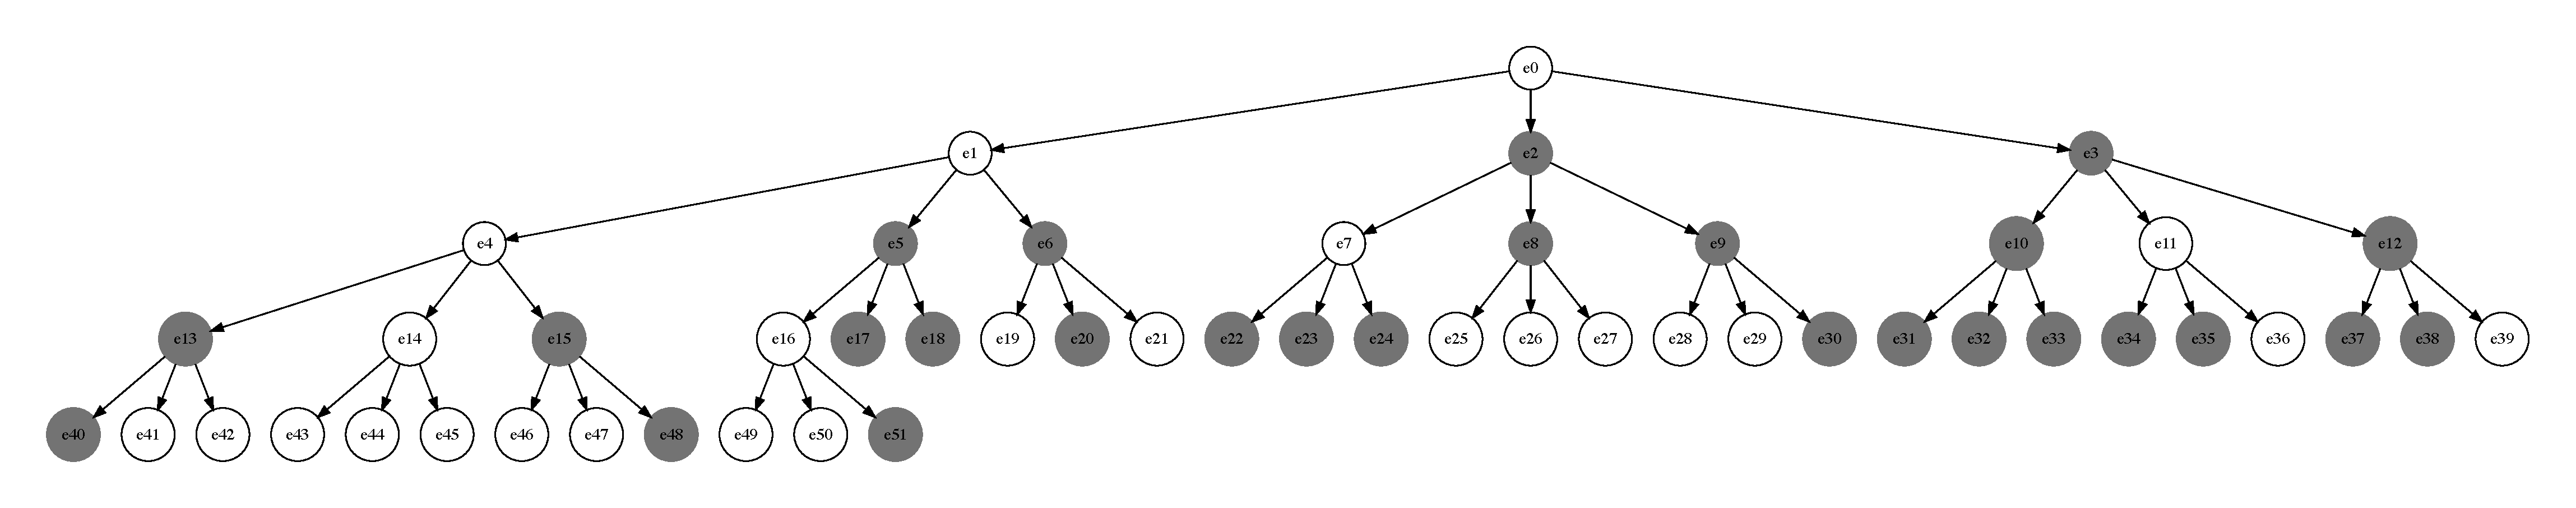
\includegraphics[width=\textwidth]{figs/Uni-hierachy.pdf}
  \end{minipage}
\end{figure}

For each employee, we use the generative model of Figure~\ref{fig:BN} to draw assignments for all the random variables. We assume that only $40\%$ of employees are qualified for promotion and regardless of their labels, employees submit only $60\%$ of their opinions. In addition, due to various personal and environmental factors, only $60\%$ of high quality employees perform well while $10\%$ of low quality employees also perform well regardless of their labels. Note that these numbers are not specific and just chosen for the framework to serve as a representative setting and a proof of concept. The conditional probability table for the opinion variable $O$ is parameterized by four values $(\theta_1, \theta_2, \theta_3, \theta_4)$ which together determine the degree of discrimination against the protected group. Since other parameters in the Bayesian network did not have a direct effect on the degree of discrimination, we fixed them to arbitrary values. 

The results presented in this section are based on an organization hierarchy  with $100$ employees where $k=5$. However, the results of the framework are not sensitive to the settings as we test the framework with various organization sizes ranging from $50$ to $500$ employees and various degree for $k$ ranging from $3$ to $10$. We generated seven datasets given the organization hierarchy using different values for the $\theta$ parameters: $(0.0,1.0,0.0,0.0)$, $(0.33,1.0,0.0,0.0)$, $(0.66,1.0,0.0,0.0)$, $(1.0,1.0,0.0,0.0)$, $(1.0,1.0,0.0,0.33)$, $(1.0,1.0,0.0,0.66)$, $(1.0,1.0,0.0,1.0)$. 
 
In the first three settings the discrimination originates from negative opinions towards qualified outgroup employees. The first setup is an extreme case where the opinion towards outgroup employees is always negative. The discrimination in the last three settings originates from positive opinions towards unqualified ingroup employees. The last setup is an extreme case where the opinion towards ingroup employees is always positive. The fourth setup represent unbiased opinions where employees are treated similarly based on their qualification. 

\paragraph{MAP Inference} We use the model presented in Table~\ref{tab:pslmodel} for MAP inference in PSL and FairPSL (recall that in FairPSL, the $\delta$-fairness constraints corresponding to one of the fairness measures are also added to the model). The observed atoms are $\textit{Manager(m,e)}$, $\textit{PositiveReview(e1,e2)}$ and labels of all employees. The truth values for all other atoms are obtained via MAP inference. We use the truth values obtained for the decision atoms $\textit{ToPromote(e)}$ to compute the fairness measures. We defined the discriminative pattern, and the protected and unprotected groups of this problem in Section~\ref{sec:formulation}.


\subsection{Evaluation results}

\begin{figure}
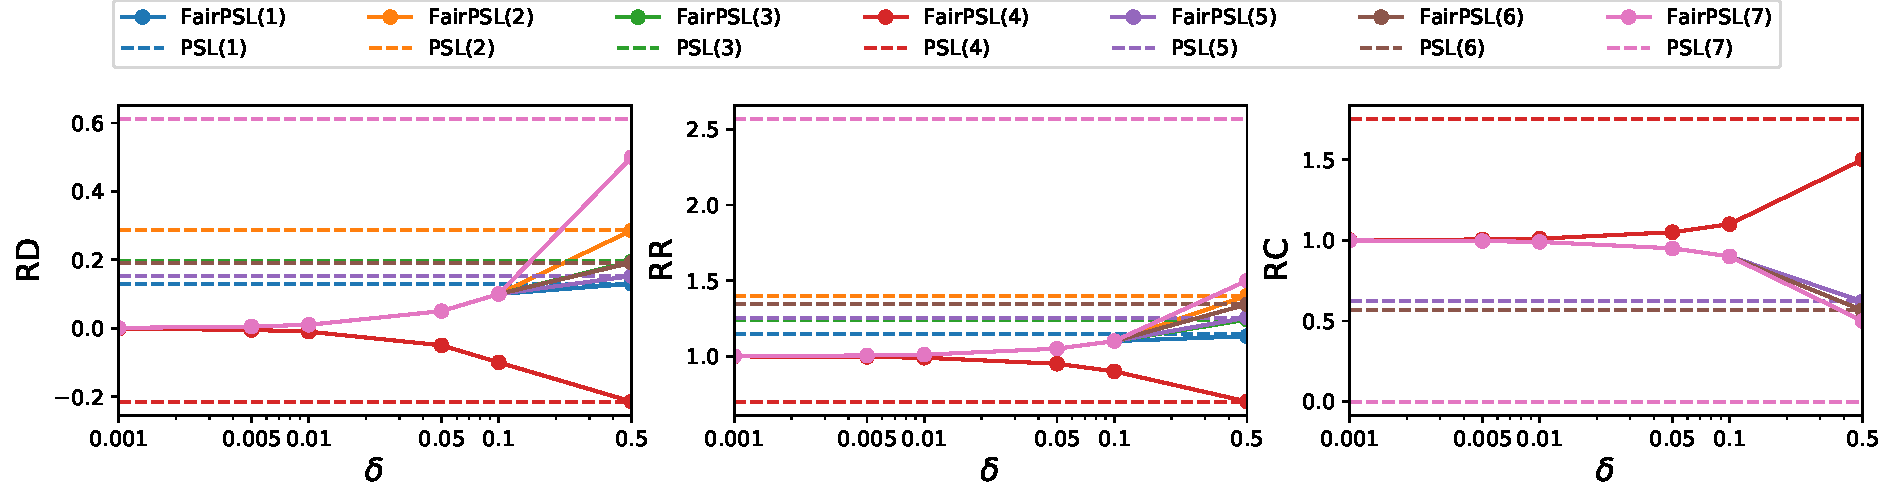
\includegraphics[width=1\linewidth]{figs/results_vis_uni_params.pdf}
\caption{\small Fairness score of predictions obtained by MAP inference of PSL and FairPSL, according to the fairness measures \emph{RD}, \emph{RR}, and \emph{RC}. The labels of datasets are mentioned with parenthesis next to the inference method. The FairPSL values of each measure are obtained by adding the $\delta$-fairness constraint of that measure.\label{fig:results}
}  
\end{figure}

To answer \textbf{Q1}, we run the MAP inference algorithm of PSL and FairPSL on seven synthetic datasets. 
We run the MAP inference of FairPSL multiple times on each dataset: For each of the three fairness measures, we add the corresponding $\delta$-fairness constraint with five thresholds $\{0.001, 0.005, 0.01, 0.05, 0.1, 0.5\}$.

Figure~\ref{fig:results} shows the fairness score of predictions in terms of the three fairness measures. As expected, tighter $\delta$-fairness constraints lead to better scores. Note that the best possible score according to RD is 0, as it computes a difference. Since RR and RC compute ratios, the best possible score according to these measures is 1. In our experiments, with any of these measures, taking $\delta = 0.001$ pushes the score of predictions to its limit.  

The $\delta$-fairness constraints modify the optimization problem of MAP inference by reducing the feasible region to solutions that conform with fairness guarantees. Research question \textbf{Q2} is concerned with the effect of this reduction on the accuracy of predictions. Note that decision quality is the same as the accuracy of predictions. To answer this question, we compare the inferred values for the decision atoms \textit{ToPromote(e)} against their actual values. These values are extracted from the known values of \textit{IsQualified(e)} according to rules 11 and 12 in Table~\ref{tab:pslmodel}. Figure~\ref{fig:accuracy} shows the area under the curve of the receiver operating characteristic~(AUC) of predicting the decision variable in three groups, namely the protected group, the unprotected group (i.e., promotion of the employees who have in-group managers), and all employees. By doing so, we make sure that our fairness constraints do not propagate bias towards either of the populations. Since the results of FairPSL with $\delta$-fairness constraints RR and RC are very similar to the results of RD, we only report the latter here.


\begin{figure}
    \centering
    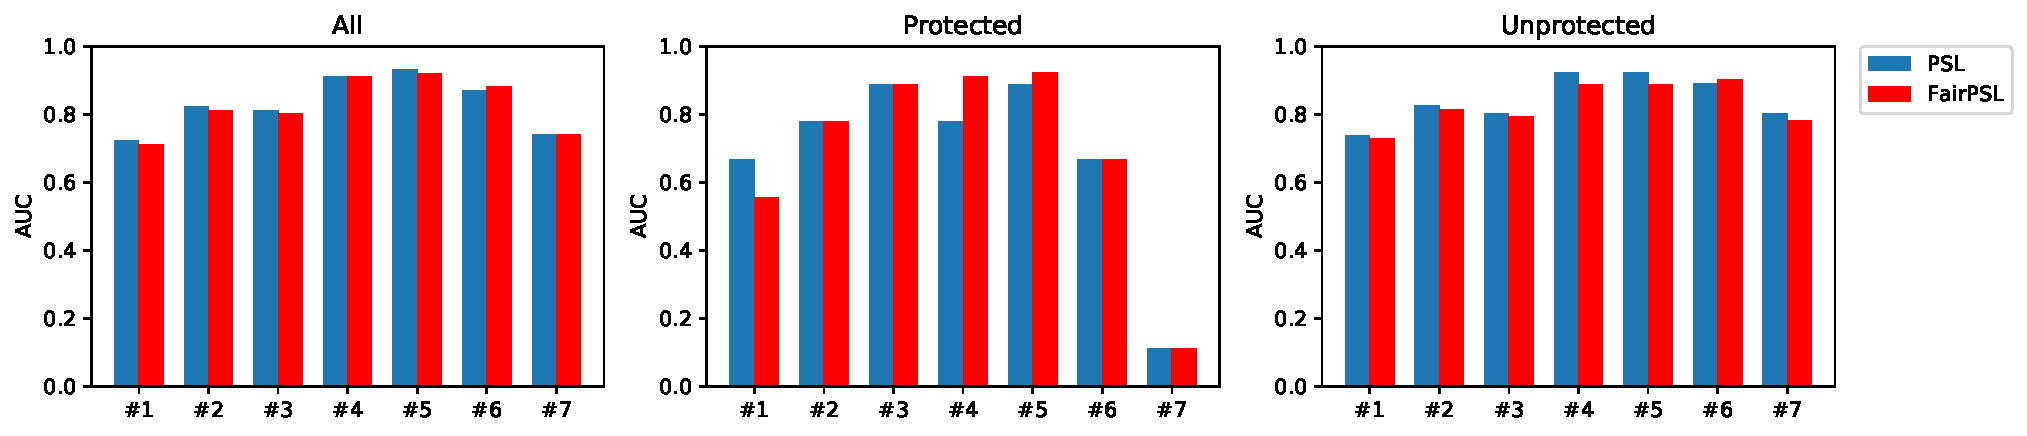
\includegraphics[width=\textwidth]{figs/roc.pdf}
    \caption{\small AUC score of predictions for truth values of unknown atoms \textit{ToPromote(e)} using MAP inference of PSL and FairPSL with $\delta$-fairness constraints $RD$ with $\delta=0.001$.}
    \label{fig:accuracy}
\end{figure}

According to Figure~\ref{fig:accuracy}, the results of both PSL and FairPSL in all seven datasets are close to each other. Note that although fairness may impose a cost in terms of overall accuracy, FairPSL often improves the accuracy of the protected class. Sometimes the overall predictions of FairPSL are even slightly better than PSL (e.g., dataset 6 and 7). As expected, the accuracy of the fourth setting where the opinions are unbiased are similar in both PSL and FairPSL. We observe that prediction of MAP inference for both FairPSL and PSL are similar, thus, in these settings at least, FairPSL guarantees fairness without hurting accuracy. Further investigation is required on the effect of the various ranges of discrimination (i.e., $\theta_1$, $\theta_2$, $\theta_3$, $\theta_4$) on the prediction results of FairPSL.



We also generate various types of organizations in which labels are not uniformly distributed, e.g., one population only occurs at the bottom levels of an organization. While we did not observe any differences in the behavior of our method with respect to accuracy and fairness measure, we found that the degree of discrimination is higher in such organizations. Further investigations on the structure of an organization on discrimination is an interesting direction for future research. 

\section{Conclusion and Future Directions}
\label{sec:conclusion}
Many applications of AI and machine learning affect peoples' lives in important ways. While there is a growing body of work on fairness in AI and ML, it assumes an individualistic notion of fairness.   In this paper, we have proposed a general framework for relational fairness which includes both a rich language for defining discrimination patterns and an efficient algorithm for performing inference subject to fairness constraints. We show our approach enforces fairness guarantees while preserving the accuracy of the predictions. 

There are many avenues for expanding on this work. For example, here we assumed that the discriminative pattern is given, however an automatic mechanism to extract discriminatory situations hidden in a large amount of decision records is an important and required task. Discrimination discovery has been studied for attribute-based fairness~\cite{pedreschi2013discovery}. An interesting next step is discrimination pattern discovery in relational data.

\section*{Acknowledgements}
This work is supported by the National Science Foundation under Grant Numbers CCF-1740850 and IIS-1703331. Golnoosh Farnadi and Behrouz Babaki are  supported by postdoctoral scholarships from IVADO through the Canada First Research Excellence Fund (CFREF) grant.

\begin{thebibliography}{10}
\itemsep=1pt 
\begin{small}

\bibitem{EUlaw}
European union legislation. (a) racial equality directive, 2000; (b) employment
  equality directive, 2000; (c) gender employment directive, 2006; (d) equal
  treatment directive (proposal), 2008.

\bibitem{UKlaw}
{UK} legislation. (a) sex discrimination act, 1975, (b) race relation act,
  1976.

\bibitem{USlaw}
United nations legislation. (a) universal declaration of human rights, 1948,
  (c) convention on the elimination of all forms of racial discrimination,
  1966, (d) convention on the elimination of all forms of discrimination
  against women, 1979.

\bibitem{alshukaili:iswc16}
Duhai Alshukaili, Alvaro A.~A. Fernandes, and Norman~W. Paton.
\newblock Structuring linked data search results using probabilistic soft
  logic.
\newblock In {\em International Semantic Web Conference {(1)}}, volume 9981 of
  {\em Lecture Notes in Computer Science}, pages 3--19, 2016.

\bibitem{bach:jmlr17}
Stephen~H. Bach, Matthias Broecheler, Bert Huang, and Lise Getoor.
\newblock Hinge-loss markov random fields and probabilistic soft logic.
\newblock {\em Journal of Machine Learning Research}, 18:109:1--109:67, 2017.

\bibitem{barocas2016big2}
Solon Barocas and Andrew~D Selbst.
\newblock Big data's disparate impact.
\newblock {\em California Law Review}, 104:671, 2016.

\bibitem{boyd2014networked}
Danah Boyd, Karen Levy, and Alice Marwick.
\newblock The networked nature of algorithmic discrimination.
\newblock In {\em Data and discrimination: Collected essays}, pages 53--57.
  2014.

\bibitem{brewer1979group}
Marilynn~B Brewer.
\newblock In-group bias in the minimal intergroup situation: A
  cognitive-motivational analysis.
\newblock {\em Psychological bulletin}, 86(2):307, 1979.

\bibitem{brewer2007social}
Marilynn~B Brewer.
\newblock The social psychology of intergroup relations: Social categorization,
  ingroup bias, and outgroup prejudice.
\newblock {\em Social Psychology: Handbook of Basic Principles}, 2007.

\bibitem{chouldechova2017fair2}
Alexandra Chouldechova.
\newblock Fair prediction with disparate impact: {A} study of bias in
  recidivism prediction instruments.
\newblock {\em CoRR}, abs/1703.00056, 2017.

\bibitem{dwork2012fairness3}
Cynthia Dwork, Moritz Hardt, Toniann Pitassi, Omer Reingold, and Richard~S.
  Zemel.
\newblock Fairness through awareness.
\newblock In {\em {ITCS}}, pages 214--226. {ACM}, 2012.

\bibitem{ebrahimi:emnlp16}
Javid Ebrahimi, Dejing Dou, and Daniel Lowd.
\newblock Weakly supervised tweet stance classification by relational
  bootstrapping.
\newblock In {\em {EMNLP}}, pages 1012--1017. The Association for Computational
  Linguistics, 2016.

\bibitem{farnadi2018fairness}
Golnoosh Farnadi, Behrouz Babaki, and Lise Getoor.
\newblock Fairness in relational domains.
\newblock In {\em AAAI/ACM Conference on AI, Ethics, and Society (AIES)}, pages
  108--114. ACM, 2018.

\bibitem{feldman2015certifying2}
Michael Feldman, Sorelle~A. Friedler, John Moeller, Carlos Scheidegger, and
  Suresh Venkatasubramanian.
\newblock Certifying and removing disparate impact.
\newblock In {\em {KDD}}, pages 259--268. {ACM}, 2015.

\bibitem{getoor2007introduction}
Lise Getoor and Ben Taskar.
\newblock {\em {Introduction to Statistical Relational Learning}}.
\newblock MIT press Cambridge, 2007.

\bibitem{hardt2016equality3}
Moritz Hardt, Eric Price, and Nati Srebro.
\newblock Equality of opportunity in supervised learning.
\newblock In {\em {NIPS}}, pages 3315--3323, 2016.

\bibitem{kamishima2011fairness}
Toshihiro Kamishima, Shotaro Akaho, and Jun Sakuma.
\newblock Fairness-aware learning through regularization approach.
\newblock In {\em ICDMW}, pages 643--650. {IEEE} Computer Society, 2011.

\bibitem{kouki:recsys15}
Pigi Kouki, Shobeir Fakhraei, James~R. Foulds, Magdalini Eirinaki, and Lise
  Getoor.
\newblock Hyper: {A} flexible and extensible probabilistic framework for hybrid
  recommender systems.
\newblock In {\em RecSys}, pages 99--106. {ACM}, 2015.

\bibitem{counterfactualfairness}
Matt~J. Kusner, Joshua~R. Loftus, Chris Russell, and Ricardo Silva.
\newblock Counterfactual fairness.
\newblock In {\em {NIPS}}, pages 4069--4079, 2017.

\bibitem{Pedreschi:2012}
Dino Pedreschi, Salvatore Ruggieri, and Franco Turini.
\newblock A study of top-k measures for discrimination discovery.
\newblock In {\em {SAC}}, pages 126--131. {ACM}, 2012.

\bibitem{pedreschi2013discovery}
Dino Pedreschi, Salvatore Ruggieri, and Franco Turini.
\newblock The discovery of discrimination.
\newblock In {\em Discrimination and Privacy in the Information Society},
  volume~3 of {\em Studies in Applied Philosophy, Epistemology and Rational
  Ethics}, pages 91--108. Springer, 2013.

\bibitem{ridgeway2004unpacking}
Cecilia~L Ridgeway and Shelley~J Correll.
\newblock Unpacking the gender system: A theoretical perspective on gender
  beliefs and social relations.
\newblock {\em Gender \& society}, 18(4):510--531, 2004.

\bibitem{sridhar:bioinformatics16}
Dhanya Sridhar, Shobeir Fakhraei, and Lise Getoor.
\newblock A probabilistic approach for collective similarity-based drug-drug
  interaction prediction.
\newblock {\em Bioinformatics}, 32(20):3175--3182, 2016.

\bibitem{verma2018fairness2}
Sahil Verma and Julia Rubin.
\newblock Fairness definitions explained.
\newblock In {\em 2018 IEEE/ACM International Workshop on Software Fairness
  (FairWare)}, pages 1--7. IEEE, 2018.

\bibitem{west2014exploiting}
Robert West, Hristo~S. Paskov, Jure Leskovec, and Christopher Potts.
\newblock Exploiting social network structure for person-to-person sentiment
  analysis.
\newblock {\em {TACL}}, 2:297--310, 2014.

\bibitem{zafar2017parity}
Muhammad~Bilal Zafar, Isabel Valera, Manuel Gomez{-}Rodriguez, Krishna~P.
  Gummadi, and Adrian Weller.
\newblock From parity to preference-based notions of fairness in
  classification.
\newblock In {\em {NIPS}}, pages 228--238, 2017.

\bibitem{zemel2013learning}
Richard~S. Zemel, Yu~Wu, Kevin Swersky, Toniann Pitassi, and Cynthia Dwork.
\newblock Learning fair representations.
\newblock In {\em {ICML} {(3)}}, volume~28 of {\em {JMLR} Workshop and
  Conference Proceedings}, pages 325--333. JMLR.org, 2013.

\end{small}
\end{thebibliography}

\end{document}

\end{article}


\begin{article}
{{\sc ModelDB}: Opportunities and Challenges in Managing Machine Learning Models}
{Manasi Vartak, Samuel Madden}
\graphicspath{{submissions/gustavo/}}
%\documentclass[11pt,dvipdfm]{article}
\documentclass[11pt]{article}
\usepackage{deauthor,times,graphicx} %required
\usepackage{amsmath,amssymb}
\usepackage{multirow}
\usepackage{algorithm}
\usepackage{algpseudocode}
\usepackage{todonotes}
\usepackage{url}

% \graphicspath{{farnadi/}}

\newtheorem{mydef}{\textbf{Definition}}
\newtheorem{myex}{\textbf{Example}}
\newtheorem{mytheorem}{\textbf{Theorem}}


\begin{document}

\title{A Declarative Approach to Fairness in Relational Domains}
\author{Golnoosh Farnadi$^{1,2}$, Behrouz Babaki$^1$, Lise Getoor$^3$\\
$^1$Polytechnique Montr\'{e}al, $^2$ Mila, $^3$ UC Santa Cruz \\
farnadig@mila.quebec, behrouz.babaki@polymtl.ca, getoor@soe.ucsc.edu}

\maketitle

\begin{abstract}
AI and machine learning tools are being used with increasing frequency for decision making in domains that affect peoples' lives such as employment, education, policing and %loan approval
financial qualifications. These uses raise concerns about biases of algorithmic discrimination and have motivated the development of fairness-aware machine learning. However, existing fairness approaches are based solely on attributes of individuals. In many cases, discrimination is much more complex, and taking into account the social, organizational, and other connections between individuals is important. We introduce new notions of fairness that are able to capture the relational structure in a domain. We use first-order logic to provide a flexible and expressive language for specifying complex relational patterns of discrimination. Furthermore, we extend an existing statistical relational learning framework, probabilistic soft logic~(PSL), to incorporate our definition of relational fairness. We refer to this fairness-aware framework FairPSL. FairPSL makes use of the logical definitions of fairnesss but also supports a probabilistic interpretation. In particular, we show how to perform maximum a posteriori~(MAP) inference by exploiting probabilistic dependencies within the domain while avoiding violations of fairness guarantees. Preliminary empirical evaluation shows that we are able to make both accurate and fair decisions.
\end{abstract}

\section{Introduction}
\label{sec:introduction}

Over the past few years, AI and machine learning have become essential components in operations that drive the modern society, e.g., in financial, administrative, and educational spheres. \emph{Discrimination} happens when qualities of individuals which are not relevant to the decision making process influence the decision. Delegating decision making to an automated process raises questions about discriminating against individuals with certain traits based on biases in the data. This is especially important when the decisions have the potential to impact the lives of individuals, for example, the decisions on granting loans, assigning credit, and employment. 

\emph{Fairness} is defined as the absence of discrimination in a decision making process. The goal of \emph{fairness-aware} machine learning is to ensure that the decisions made by an algorithm do not discriminate against a population of individuals~\cite{feldman2015certifying2,boyd2014networked,hardt2016equality3}. Fairness has been well studied in the social sciences and legal scholarship (for an in-depth review see~\cite{barocas2016big2}), and there is emerging work on fairness-aware ML within the AI and computer science communities. For example, fairness through awareness/Lipschitz property~\cite{dwork2012fairness3}, individual fairness~\cite{zemel2013learning}, statistical parity/group fairness~\cite{kamishima2011fairness}, counterfactual fairness~\cite{counterfactualfairness}, demographic parity/disparate impact~\cite{feldman2015certifying2,chouldechova2017fair2}, preference-based fairness~\cite{zafar2017parity}, and equality of opportunity~\cite{hardt2016equality3}.

The existing work in fairness-aware machine learning is based on a definition of discrimination where a decision is influenced by an \emph{attribute} of an individual. An attribute value upon which discrimination is based (such as gender, race, or religion) is called a \emph{sensitive attribute}. The sensitive attribute defines a population of vulnerable individuals known as the \emph{protected group}. A fair decision-making process treats the protected group the same as the \emph{unprotected group}. 

However, in many social contexts, discrimination is the result of complex interactions and can not be described solely in terms of attributes of an individual. For example, consider an imaginary scenario in an organization in which younger female workers who have older male supervisors have lower chances of promotion than their male counterparts.\footnote{Of course, many other patterns may be possible: female bosses may promote female subordinates and discriminate against male workers, or male bosses may promote female employees.  Our goal is to provide a general framework which is able to describe arbitrarily complex discrimination patterns.} 
 This discrimination pattern involves two attributes of the individual (gender and age), a relationship with another individual (supervisor), and two attributes of the second individual. Addressing such complex cases poses two challenges. First, the concepts of discrimination and fairness need to be extended to capture not only attributes of individuals but also the relationships between them. Second, a process is required that ensures that fair decisions are made about individuals who are affected by such patterns. In this paper we address both of these challenges.
We use first-order logic (FOL) to extend the notion of fairness to the relational setting. FOL is an expressive representation for relational problems which is also widely used for learning in relational domains. Moreover, we extend an existing framework for statistical relational learning~\cite{getoor2007introduction} called probabilistic soft logic (PSL)\footnote{http://psl.linqs.org/}~\cite{bach:jmlr17}. PSL combines logic and probability for learning and reasoning over uncertain relational domains. One of the most common reasoning tasks in PSL is called maximum a posteriori (MAP) inference, which is performed by finding the most probable truth values for unknowns over a set of given evidence. We develop a new MAP inference algorithm which is able to maximize the a posteriori values of unknown variables \emph{subject to} fairness guarantees. An early version of this paper which this work builds upon and extends appeared in~\cite{farnadi2018fairness}.

\looseness-1
Our contributions are as follows: 1) we propose fairness-aware machine learning for the relational setting; 2) we extend PSL into a fairness-aware framework called FairPSL which can represent the logical definition of fairness; 3) we develop a new MAP inference algorithm which is able to maximize the posteriori values of unknown variables \emph{subject to} fairness guarantees; 4) we empirically evaluate our proposed framework on synthetic data. 

\section{Motivation}
\label{sec:motivation}

Discrimination in social contexts have been studied in the field of social psychology~\cite{brewer2007social,brewer1979group,ridgeway2004unpacking}. There is a large literature on various aspects of relational bias in social contexts such as \emph{in-group-out-group bias}, \emph{gender bias}, and \emph{ethnicity-based favoritism} that can result in discrimination. 
As an example, consider gender bias in the workplace that reflects stereotypically masculine criteria and male-based favoritism. Such gender bias 
typically places women in lower positions and negatively impacts their opportunities. Further, lack of women in leadership positions may affect the promotion of women and results in a glass ceiling that keeps women from rising beyond a certain level in the hierarchy. This scenario shows that considering  protected attributes such as gender is not always sufficient to detect the source of bias and avoid discrimination, one also has to consider the relational information, in this case the organization hierarchy. Note that this can be generalized to any ingroup/outgroup scenario where the sensitive attribute could be race, religion, age, marital-status, etc.

The existing work on designing fair algorithms in machine learning exclusively focuses on \emph{attribute-based fairness}, which is based on the following assumptions: First, there is an assumption that the individuals (sometimes referred to as units or entities) are independent and described by simple attribute vectors. Second, the group for which one wishes to ensure fairness (known as the \emph{protected group}) is defined on the basis of some attribute values. Finally, there is a decision that is associated with each individual, and the goal is to ensure that members of the protected group are subject to a fair decision (we discuss different fairness measures in Section~\ref{sec:fairnessmeasure}).  We illustrate  attribute-based fairness in the following example. 

\begin{myex}[Loan Processing]
\label{ex:loan}
A bank bases its decisions about granting a loan on attributes of the applicant. The goal is to decide whether to grant a loan to an applicant using a predictive model. The bank needs to ensure that the obey fair lending practices and ensure that gender, race, sexual orientation of applicants has no influence on the decision. In this scenario, the protected group is the historically disadvantaged applicants.  
\end{myex}
The current fairness-aware machine learning techniques are not capable of modeling relations and hence cannot be used to make the decision making model fair. However, in many decision making scenarios, especially in social and organizational settings, the domain is relational, and the protected group itself might be best represented using a relational definition. We illustrate this setting in the following scenario:
\begin{myex}[Performance Review]
\label{ex:review}
Consider an organization where decisions about the promotion of employees is based on two criteria: 1) an objective performance measure, and 2) the opinion of their direct and indirect managers above them. The opinions are inferred from the performance reviews which are collected periodically. Not every manager can submit a review for all its subordinates, this is especially the case for top-level managers who have a large number of subordinates. Hence, the opinions of managers are collectively inferred from the opinions of their sub-ordinates. However, some employees may be biased, and judge other employees unfavorably, by favoring employees who are similar to themselves (same gender, race, religion, etc.) over employees who are dissimilar. The organization needs to ensure that promotion of employees do not have any relational bias caused by in-group-out-group favoritism.

\end{myex}
Example~\ref{ex:review} describes a prediction problem over a database that consists of relations between employees. Such prediction tasks are best handled by techniques from the relational learning domain. To ensure fair prediction in such settings, we need to extend the notion of \emph{attribute-based fairness} to \emph{relational fairness}. Throughout this paper, we use the performance review problem as a running example for relational fairness.

\section{Fairness Formalism}
\label{sec:formulation}

A representation that can describe different types of entities and different relationships between them is called relational. In this section, we use first-order logic to define relational fairness. We employ first-order logic as an expressive representation formalism which can represent objects and complex relationships between them. We start by defining an atom:

\begin{mydef}[Atom]
An atom is an expression of the form $P(a_1, a_2, \ldots, a_n)$ where each argument $a_1, a_2,$ $\ldots,$ $a_n$ is either a constant or a variable. The finite set of all possible substitutions of a variable to a constant for a particular variable $a$ is called its \textit{domain} $D_{a}$. If all variables in $P(a_1, a_2, \ldots, a_n)$ are substituted by some constant from their respective domain, then we call the resulting atom a \textit{ground atom}. 
\end{mydef}

\begin{myex}
In our loan processing problem (Example~\ref{ex:loan}), we can represent applicants' attributes by atoms. For instance, atom $Female(v)$ indicates whether or not applicant $v$ is female. Similarly, we can represent relations with atoms. In the performance review problem in Example~\ref{ex:review} the atom $Manager(m,e)$ indicates whether or not employee $m$ is a direct or indirect manager of employee $e$.
\end{myex}

The relational setting provides the flexibility to express complex definitions with formulae.

\begin{mydef}[Formula] 
A formula is defined by induction: every atom is a formula. If $\alpha$ and $\beta$ are formulae, then $\alpha \vee \beta$, $\alpha \wedge \beta$, $\neg \alpha$, $\alpha \rightarrow \beta$ are formulae. If $x$ is a variable and $\alpha$ is a formula, then the quantified expressions of the form $\exists x$ $\alpha$ and $\forall x$ $\alpha$ are formulae.    
\end{mydef}

To characterize groups of individuals based on a formula, we define the notion of \emph{population}.

\begin{mydef}[Population]
We denote formula $F$ which has only one free variable $v$ (i.e., other variables in $F$ are quantified) by $F[v]$. The population defined by $F[v]$ is the set of substitutions of $v$ for which $F[v]$ holds.   
\end{mydef}


\begin{myex}
\label{ex:disformula}
Consider the formula $F[v] := \forall u, \, \textit{Manager}(u,v) \rightarrow \neg \textit{SameGroup}(u, v)$. The population specified by this formula is the set of individuals all of whose managers belong to a group different from theirs. 
\end{myex}

The truth value of a formula is derived from the truth value of atoms that it comprises, according to the rules of logic. Each possible assignment of truth values to ground atoms is called an \emph{interpretation}. 


\begin{mydef}[Interpretation]
An interpretation $I$ is a mapping that associates a truth value $I(P)$ to each ground atom $P$. For Boolean truth values, $I$ associates true to 1 and false to 0 truth values. For soft logic (see Definition~\ref{def:softlogic}) $I$ maps each ground atom $P$ to a truth value in interval $[0, 1]$.
\end{mydef}

In attribute-based fairness, it is assumed that there is a certain attribute of individuals, i.e, the sensitive attribute,  that we do not want to affect a decision. Gender, race, religion and marital status are examples of sensitive attributes. Discrimination has been defined in social science studies as a treatment in favor or against a group of individuals given their sensitive attribute. This group of individuals is the protected group. 

In a relational setting, both the sensitive attributes of an individual and their participation in various relations may have an undesired effect on the final decision. We characterize the protected group in a relational setting by means of a population. In practice, we are often interested in maintaining fairness for a specific population such as applicants, students, employees, etc. This population is then partitioned into the protected and unprotected groups. We define a \emph{discriminative pattern} which is a pair of formulae to capture these groups: 1) $F_1[v]$: to specify the difference between the protected and unprotected groups and 2) $F_2[v]$: to specify the population over which we want to maintain fairness. 

\begin{mydef}[Discriminative pattern]
A discriminative pattern is a pair $\textit{DP}[v]:=(F_1[v], F_2[v])$ , where $F_1[v]$ and $F_2[v]$ are formulae.
\end{mydef}

\begin{myex}
\label{ex:pattern}
The two formulae in the discrimination pattern $\textit{DP}[v]:= \big((\forall u, \,  \textit{Manager}(u,v) \rightarrow  \neg \textit{SameGroup}(u, v)),$ $\textit{Employee}(v)\big)$ specify two populations, namely all employees and those employees who belong to a group different from their managers.
\end{myex}

Given the definition of the discriminative pattern, we have a rich language to define the scope of the protected and unprotected groups in a relational setting.

\begin{mydef}[Protected group] Given an interpretation $I$, the protected group is a population of the form:
{$$PG :=\{ v : F_1[v] \wedge F_2[v]\}$$}
which is defined as the set of all instances hold for variable $v$ for which $F_1[v] \wedge F_2[v]$ is true under interpretation $I$, that is, $I(F_1[v] \wedge F_2[v]) = 1$. 
Similarly, the \emph{unprotected group} is a population of the form: 
{$$UG := \{ v : \neg F_1[v] \wedge  F_2[v]\}$$}
which is defined as the set of all instances hold for variable $v$ 
for which $I(\neg F_1[v] \wedge F_2[v]) = 1$. 
\end{mydef}

\begin{myex}
The protected group of the discrimination pattern specified in Example~\ref{ex:pattern} is {$PG := \big\{ v : \big(\forall u, \,$ $ \textit{Manager}(u, v) \rightarrow \neg \textit{SameGroup}(u, v)\big) \wedge \textit{Employee}(v) \big\}$} and the unprotected group is {$UG :=  \big\{ v:  \big(\exists u, \, \textit{Manager}(u,v) \wedge \textit{SameGroup}(u, v)\big) \wedge \textit{Employee}(v) \big\}$}. This means our protected group is the set of employees belonging to a group different from their managers,
and our unprotected group consists of other employees. 
\end{myex}

Discrimination is defined in terms of a treatment or decision that distinguishes between the protected and unprotected groups. Here we define the \emph{decision} atom.
\begin{mydef}[Decision atom] A decision atom $d(v)$ is an atom containing exactly one variable $v$ that specifies a decision affecting the protected group which is defined either by law or end-user.
\end{mydef}
\begin{myex}
The decision atom ${\textit ToPromote}(v)$ indicates whether or not $v$ receives a promotion.
\end{myex}

Note that the fairness formulation in this section is designed for the relational setting, however relational fairness subsumes the attribute-based fairness such that: a sensitive attribute is defined by an atom with one argument and $F_2[v]$ in discrimination pattern is $\textit{Applicant}(v)$. For example, discrimination pattern of our loan processing problem in Example~\ref{ex:loan} is of the form $\textit{DP} := ( \textit{Female}(v), \textit{Applicant}(v))$ that denotes female applicants as the protected group (i.e., $PG :=  \{ v: \textit{Female}(v) \}$) and male applicants as the unprotected group (i.e., $UG := \{ v: \neg \textit{Female}(v)\}$).


\section{Fairness Measures}
\label{sec:fairnessmeasure}

Over the past few years, many fairness measures have been introduced~\cite{verma2018fairness2}. An important class of these measures are \emph{group fairness} measures which quantify the inequality between different subgroups. Some of the most popular measures in this class include \emph{equal opportunity}, \emph{equalized odds}, and \emph{demographic parity}~\cite{hardt2016equality3}. In this paper we restrict our focus to the latter. In an attribute-value setting, demographic parity means that the decision should be independent of the protected attributes. Assume that binary variables $A$ and $C$ denote the decision and protected attributes, and the preferred value of $A$ is one. Demographic parity requires that:

\begin{equation*}
    P(A=1 | C=0) = P(A=1 | C=1)
\end{equation*}

We will now generalize this measure to the relational setting using the notations defined in Section~\ref{sec:formulation}. Let $a$ and $c$ denote the counts of denial (i.e., negative decisions) for protected and unprotected groups, and $n_{1}$ and $n_{2}$ denote their sizes, respectively. Given the decision atom $d(v)$, discriminative pattern $\textit{DP}(F_1[v], F_2[v])$, and interpretation $I$, these counts are computed by the following equations: 
{
\begin{flalign}
    & a \equiv \sum_{v \in D_v} I\big( \neg d(v) \wedge  F_1[v] \wedge F_2[v]) \label{eq:a}\\
    & c \equiv \sum_{v \in D_v} I\big( \neg d(v) \wedge  \neg F_1[v] \wedge  F_2[v]) \label{eq:c}\\
    & n_{1} \equiv \sum_{v \in D_v} I\big(F_1[v] \wedge F_2[v]) \label{eq:n1}\\
    & n_{2} \equiv \sum_{v \in D_v} I\big(\neg F_1[v] \wedge  F_2[v]) \label{eq:n2}
\end{flalign}}
The proportions of denying for protected and unprotected groups are $p_1 = \frac{a}{n_1}$ and $p_2 = \frac{c}{n_2}$, respectively. There are a number of data-driven measures~\cite{Pedreschi:2012} which quantify demographic disparity and can be defined in terms of $p_1$ and $p_2$:
\begin{itemize}
    \item \textbf{Risk difference}: $RD = p_1 - p_2$, also known as absolute risk reduction. 
    \item \textbf{Risk Ratio}: $RR = \frac{p_1}{p_2}$, also known as relative risk. 
    \item \textbf{Relative Chance}: $RC = \frac{1 - p_1}{1 - p_2}$ also, known as selection rate.
\end{itemize}
These measures have been used in the legal systems of European Union, UK, and US~\cite{EUlaw,UKlaw,USlaw}. Notice that RR is the ratio of the proportion of benefit denial between the protected and unprotected groups, while RC is the ratio of the proportion of benefit granted. Finally, we introduce the notion of $\delta$-fairness.

\begin{mydef}[$\delta$-fairness]
If a fairness measure for a decision making process falls within some $\delta$-window, then the process is \emph{$\delta\text{-fair}$}. Given $0 \leq \delta \leq 1$, the  $\delta$-windows for measures RD/RR/RC are defined as:
{\begin{flalign*}
	     - \delta \leq &RD \leq \delta \\
	     1- \delta \leq &RR \leq 1+ \delta\\
	     1- \delta \leq &RC \leq 1+ \delta
	\end{flalign*}}
\end{mydef}

To overcome the limitations of attribute-based fairness, we introduce a new statistical relational learning~(SRL) framework~\cite{getoor2007introduction} suitable for modelling fairness in relational domain. In the next section, we review probabilistic soft logic~(PSL). We then extend PSL with the definition of relational fairness introduced above in Section~\ref{sec:fairMAP}. Our fairness-aware framework, ``FairPSL'', is the first SRL framework that performs fair inference. 

\section{Background: Probabilistic Soft Logic}
\label{sec:psl}

In this section, we review the syntax and semantics of PSL, and in the next section we extend MAP inference in PSL with fairness constraints to define MAP inference in FairPSL.

PSL is a probabilistic programming language for defining hinge-loss Markov random fields~\cite{bach:jmlr17}. Unlike other SRL frameworks whose atoms are Boolean, atoms in PSL can take continuous values in the interval $[0,1]$. PSL is an expressive modeling language that can incorporate domain knowledge with first-order logical rules and has been used successfully in various domains, including bioinformatics~\cite{sridhar:bioinformatics16}, recommender systems~\cite{kouki:recsys15}, natural language processing~\cite{ebrahimi:emnlp16}, information retrieval~\cite{alshukaili:iswc16}, and social network analysis~\cite{west2014exploiting}, among many others. 
 
A PSL model is defined by a set of first-order logical rules called \emph{PSL rules}.

\begin{mydef} [PSL rule] a PSL rule $r$ is an expression of the form:
{\begin{equation}
\lambda_{r}: T_1 \land T_2 \land \ldots \land T_w \rightarrow H_1 \vee H_2 \vee \ldots \vee H_l
\end{equation}}

where { $T_1, T_2, \ldots, T_w, H_1, H_2, \ldots, H_l$} are atoms or negated atoms and { $\lambda_{r} \in \mathbb{R}^{+} \cup \infty$} is the weight of the rule $r$.  We call { $T_1 \land T_2 \land \ldots \land T_w$} the body of $r$ ($r_{body}$), and { $H_1 \vee H_2 \vee \ldots \vee H_l$} the head of $r$ ($r_{head}$).
\end{mydef}


Since atoms in PSL take on continuous values in the unit interval $[0,1]$, next we define soft logic to calculate the value of the PSL rules under an interpretation $I$.

\begin{mydef}[Soft logic]
\label{def:softlogic}
The ({$\tilde{\wedge}$}) and ({$\tilde{\vee}$}) and negation ({$\tilde{\neg}$}) are defined as follows. For {$m, n \in [0,1]$} we have: {$m \tilde{\wedge} n = \max(m+n -1, 0)$}, {$m \tilde{\vee} n = \min(m+n , 1)$} and {$\tilde{\neg} m = 1 - m$}. The $\, \tilde{} \,$ indicates the relaxation over Boolean values.
\end{mydef}

The probability of truth value assignments in PSL is determined by the rules' \emph{distance to satisfaction}.

\begin{mydef}[The distance to satisfaction]
The distance to satisfaction $d_{r}(I)$ of a rule $r$ under an interpretation $I$ is defined as:
{
\begin{equation}
d_{r}(I) = \max\{0, I(r_{body})-I(r_{head})\}
\end{equation}}
\end{mydef}

By using Definition~\ref{def:softlogic}, one can show that the closer the interpretation of a grounded rule $r$ is to 1, the smaller its distance to satisfaction. A PSL model induces a distribution over interpretations $I$. Let $R$ be the set of all grounded rules, then the probability density function is:
{
\begin{equation}
f(I) ={\frac{1}{Z}} \exp[-\sum_{r\in R} \lambda_{r}(d_{r}(I))^p]
\label{eq:potential}
\end{equation}
}
\noindent where { $\lambda_{r}$} is the weight of rule $r$, {
$Z = \int_{I} \exp[ -\sum_{r\in R} \lambda_{r}(d_{r}(I))^p]$
} is a normalization constant, and { $p \in \{1,2\}$} provides a choice of two different loss functions, $p=1$ (i.e., linear), and $p=2$ (i.e, quadratic). These probabilistic models are instances of hinge-loss Markov random fields~(HL-MRF)~\cite{bach:jmlr17}. The goal of maximum a posteriori (MAP) inference is to find the most probable truth assignments $I_{\textit{MPE}}$ of unknown ground atoms given the evidence which is defined by the interpretation $I$. Let $X$ be all the evidence, i.e., $X$ is the set of ground atoms such that $\forall x \in X, I(x)$ is known, and let $Y$ be the set of ground atoms such that $\forall y \in Y, I(y)$ is unknown. Then we have
{
\begin{equation}
I_{\textit{MAP}}(Y) = \textit{arg}\max_{I(Y)} P(I(Y)|I(X))
\end{equation}}
Maximizing the density function in Equation~\ref{eq:potential} is equivalent to minimizing the weighted sum of the distances to satisfaction of all rules in PSL. 

\begin{table*}[t]
    \centering
    \begin{tabular}{|lll|}
    \hline
    &&\\
    $R1$ & $\lambda_1$ &: $\textit{IsQualified}(e) \rightarrow \textit{HighPerformance}(e)$ \\
    $R2$ & $\lambda_1$ &: $\neg \textit{IsQualified}(e) \rightarrow \neg \textit{HighPerformance}(e)$ \\
    $R3$ & $\infty$ &: $\textit{PositiveReview}(e1, e2) \rightarrow \textit{PositiveOpinion}(e1, e2)$ \\
    $R4$ & $\infty$ &: $\neg \textit{PositiveReview}(e1, e2) \rightarrow \neg \textit{PositiveOpinion}(e1, e2)$ \\
    $R5$ & $\lambda_1$ &: $\textit{PositiveOpinion}(e1, e2) \wedge \textit{Manager}(m, e1) \rightarrow \textit{PositiveOpinion}(m, e2)$ \\
    $R6$ & $\lambda_1$ &: $\neg \textit{PositiveOpinion}(e1, e2) \wedge \textit{Manager}(m, e1) \rightarrow \neg \textit{PositiveOpinion}(m, e2)$ \\
    $R7$ & $\lambda_1$ &: $\textit{PositiveOpinion}(m, e) \wedge \textit{Manager}(m, e) \rightarrow \textit{IsQualified}(e)$ \\
    $R8$ & $\lambda_1$ &: $\neg \textit{PositiveOpinion}(m, e) \wedge \textit{Manager}(m, e) \rightarrow \neg \textit{IsQualified}(e)$ \\
    $R9$ &  $\lambda_1$ &: $\neg \textit{ToPromote}(e)$\\
    $R10$ & $\infty$ &: $\textit{IsQualified}(e) \rightarrow \textit{ToPromote}(e)$ \\
    $R11$ & $\infty$ &: $\neg \textit{IsQualified}(e) \rightarrow \neg \textit{ToPromote}(e)$ \\
    &&\\
    \hline
    \end{tabular}
    \caption{\small A simplified PSL model for the \emph{Performance Reviewing} problem}
    \label{tab:pslmodel}
\end{table*}

\begin{myex}
\label{ex:pslmodel}
The simplified PSL model for the performance reviewing problem in Example\ref{ex:review} is given in Table~\ref{tab:pslmodel}. The goal of MAP inference for this problem is to infer employees to promote. We simplified the model by assigning the same weight to all soft rules (i.e., $\lambda_i= 1$ where $i=\{1,2,5,6,7,8,9\}$). Below we explain the meaning of each rule in the model.

Rule $R1$ indicates that qualified employees have high performance and similarly rule $R2$ expresses that a negative qualification of employees is derived from their low performance. Rules $R5$ and $R6$ presents the propagation of opinion from bottom to top of the organizational hierarchy, i.e., managers have similar opinions towards employees given the opinions of their sub-ordinate managers. And rules $R7$ and $R8$ indicate that the positive/negative opinion of direct/indirect managers derive from the qualification of an employee. Rule $R9$ indicates the prior that not all employees get promoted. We also have four hard constraints (i.e., rules $R3$, $R4$, $R10$ and $R11$) where the weight of the rules are $\infty$. Rules $R3$ and $R4$ indicate that submitted positive/negative reviews should reflect positive/negative opinions. And two rules $R10$ and $R11$ show that a highly qualified employee should get promoted. 
\end{myex}

\section{Fairness-aware PSL (FairPSL)}
\label{sec:fairMAP}

The standard MAP inference in PSL aims at finding values that maximize the conditional probability of unknowns. Once a decision is made according to these values, one can use the fairness measure to quantify the degree of discrimination. A simple way to incorporate fairness in MAP inference is to add the $\delta$-fairness constraints to the corresponding optimization problem.   

Consider risk difference, $\textit{RD}$, where $\textit{RD} \equiv \frac{\mathbf{a}}{n_1} - \frac{\mathbf{c}}{n_2}$. The $\delta$-fairness constraint $-\delta \leq \textit{RD} \leq \delta$ can be encoded as the following constraints:
{\begin{align}
    & n_2 \mathbf{a} - n_1 \mathbf{c} - n_1 n_2 \delta \leq 0 \label{eq:RD1}\\
    & n_2 \mathbf{a} - n_1 \mathbf{c} + n_1 n_2 \delta \geq 0
\end{align}}
Similarly, from $\textit{RR} \equiv \frac{\mathbf{a} / n_1}{\mathbf{c} / n_2}$ and the $\delta$-fairness constraint $1 - \delta \leq \textit{RR} \leq 1 + \delta$ we obtain:
{\begin{align}
    & n_2 \mathbf{a} - (1 + \delta) n_1 \mathbf{c} \leq 0 \\
    & n_2 \mathbf{a} - (1 - \delta) n_1 \mathbf{c} \geq 0
\end{align}}
And finally, $\textit{RC} \equiv \frac{1 - \mathbf{a} / n_1}{1 - \mathbf{c} / n_2}$ and the $\delta$-fairness constraint $1 - \delta \leq \textit{RC} \leq 1 + \delta$ gives:
{ \begin{align}
    & - n_2 \mathbf{a} + (1 + \delta) n_1 \mathbf{c} - \delta n_1 n_2 \leq 0 \\
    & - n_2 \mathbf{a} + (1 - \delta) n_1 \mathbf{c} + \delta n_1 n_2 \geq 0 \label{eq:RC2}
\end{align}}
A primary advantage of PSL over similar frameworks is that its MAP inference task reduces to a convex optimization problem which can be solved in polynomial time. To preserve this advantage, we need to ensure that the problem will remain convex after the addition of $\delta$-fairness constraints. 

\begin{mytheorem}
The following condition is sufficient for preserving the convexity of MAP inference problem after addition of $\delta$-fairness constraints: The formulae $F_1[v]$ and $F_2[v]$ do not contain an atom $y \in Y$ and all atoms in $F_1[v]$ and $F_2[v]$ have values zero or one.
\end{mytheorem}
\begin{proof}
Since $I(F_1[v])$ and $I(F_2[v])$ do not depend on $I(Y)$, the values $n_{1}$ and $n_{2}$ are constants that can be computed in advance. Let us define the sets $D_v^a = \{ v \in D_v : F_1[v] \wedge F_2[v] \, \text{is true} \}$ and $D_v^c = \{ v \in D_v : \neg F_1[v] \wedge F_2[v] \, \text{is true} \}$. Since $F_1[v]$ and $F_2[v]$ can be only zero or one, we can rewrite the equations~\ref{eq:a} and \ref{eq:c} as:
{
\begin{align*}
    & \mathbf{a} = \sum_{v \in D_v^a} I(\neg d(v)) = |D_v^a| - \sum_{v \in D_v^a} I(d(v))\\
    & \mathbf{c} = \sum_{v \in D_v^c} I(\neg d(v)) = |D_v^c| - \sum_{v \in D_v^c} I(d(v))
\end{align*}}
\noindent which indicates that $\mathbf{a}$ and $\mathbf{c}$ can be expressed as linear combinations of variables in the optimization problem. This means that constraints~\ref{eq:RD1}-\ref{eq:RC2} are linear. Hence, addition of these constraints preserves the convexity of the optimization problem. 
\end{proof}

\section{Experiments}
\label{sec:experiment}

\begin{figure}
  \begin{minipage}[c]{0.6\textwidth}
    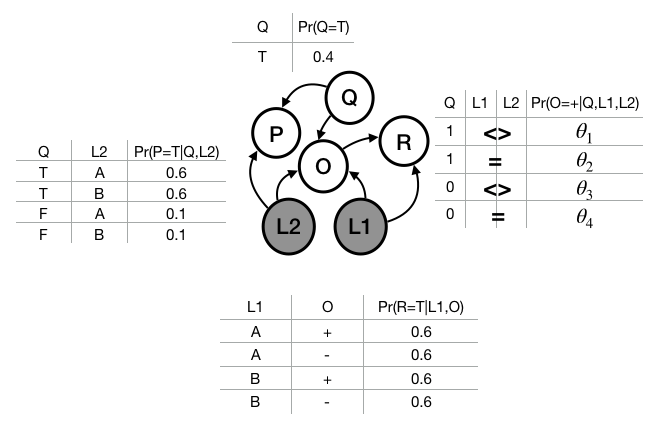
\includegraphics[width=\textwidth]{figs/BN.png}
  \end{minipage}\hfill
  \begin{minipage}[c]{0.45\textwidth}
    \caption{
        \small The model used for generating the datasets. There are four binary random variables, P, Q, O, and R. \textbf{P}: indicates whether or not the employee has high performance; \textbf{Q}: indicates whether or not an employee has high qualification; \textbf{O}: indicates whether or not the colleague submits the positive opinion towards the employee;  \textbf{R}: indicates whether or not the colleague has a positive opinion towards the employee;  \textbf{L1, L2}: indicates the label of the review provider and review receiver (observed).
    } \label{fig:BN}
  \end{minipage}
\end{figure}

We show the effectiveness of FairPSL by performing an empirical evaluation. We investigate two research questions in our experiments:
\begin{description}
\item[Q1] What is the effect of the fairness threshold $\delta$ on the fairness measures $RD/RC/RR$?
\item[Q2] How is decision quality affected by imposing $\delta$-fairness constraints?
\end{description}

Note that although we present the result for specific parameters of the framework in this section, we ran extensive analysis and the results we present are representative. We implemented the MAP inference routines of PSL and FairPSL in Python, using Gurobi-8.1\footnote{\url{www.gurobi.com}} as the backend solver. The FairPSL code, code for the data generator and data is publicly available\footnote{https://github.com/gfarnadi/FairPSL}. 

\subsection{Data generation}
  
We evaluate the FairPSL inference algorithm on synthetic datasets representing the performance review scenario (introduced in Example~\ref{ex:review}). The organization hierarchy is generated synthetically. 
The organization hierarchy generator is parameterized by two numbers: the number of employees in the organization ($n$) and the number of employees managed by each manager ($k$). Each employee is randomly assigned with a label \emph{A} or \emph{B}. An examples organization hierarchy with $n$=50 and $k$=3 is shown in Figure~\ref{fig:hierachy}.

\begin{figure}
  \begin{minipage}[c]{0.3\textwidth}
    \caption{
        \small An example of an organizational hierarchy with five levels and 50 employees with k=3. Each employee either has label A (shown with grey) or B (shown with white).
    }\label{fig:hierachy} 
	\end{minipage} \hfill
    \begin{minipage}[c]{0.7\textwidth}
    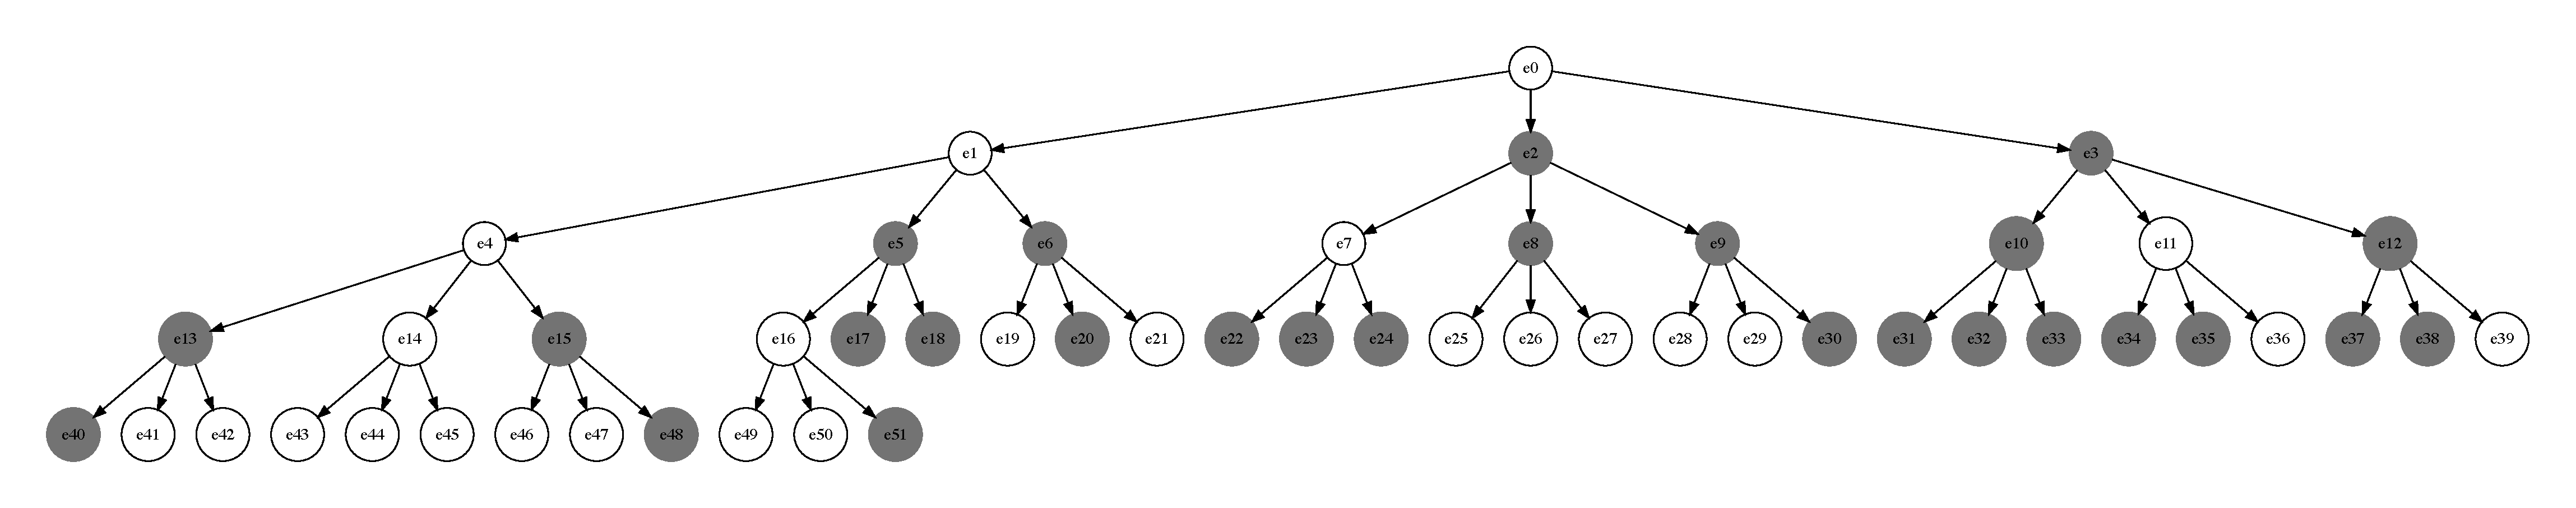
\includegraphics[width=\textwidth]{figs/Uni-hierachy.pdf}
  \end{minipage}
\end{figure}

For each employee, we use the generative model of Figure~\ref{fig:BN} to draw assignments for all the random variables. We assume that only $40\%$ of employees are qualified for promotion and regardless of their labels, employees submit only $60\%$ of their opinions. In addition, due to various personal and environmental factors, only $60\%$ of high quality employees perform well while $10\%$ of low quality employees also perform well regardless of their labels. Note that these numbers are not specific and just chosen for the framework to serve as a representative setting and a proof of concept. The conditional probability table for the opinion variable $O$ is parameterized by four values $(\theta_1, \theta_2, \theta_3, \theta_4)$ which together determine the degree of discrimination against the protected group. Since other parameters in the Bayesian network did not have a direct effect on the degree of discrimination, we fixed them to arbitrary values. 

The results presented in this section are based on an organization hierarchy  with $100$ employees where $k=5$. However, the results of the framework are not sensitive to the settings as we test the framework with various organization sizes ranging from $50$ to $500$ employees and various degree for $k$ ranging from $3$ to $10$. We generated seven datasets given the organization hierarchy using different values for the $\theta$ parameters: $(0.0,1.0,0.0,0.0)$, $(0.33,1.0,0.0,0.0)$, $(0.66,1.0,0.0,0.0)$, $(1.0,1.0,0.0,0.0)$, $(1.0,1.0,0.0,0.33)$, $(1.0,1.0,0.0,0.66)$, $(1.0,1.0,0.0,1.0)$. 
 
In the first three settings the discrimination originates from negative opinions towards qualified outgroup employees. The first setup is an extreme case where the opinion towards outgroup employees is always negative. The discrimination in the last three settings originates from positive opinions towards unqualified ingroup employees. The last setup is an extreme case where the opinion towards ingroup employees is always positive. The fourth setup represent unbiased opinions where employees are treated similarly based on their qualification. 

\paragraph{MAP Inference} We use the model presented in Table~\ref{tab:pslmodel} for MAP inference in PSL and FairPSL (recall that in FairPSL, the $\delta$-fairness constraints corresponding to one of the fairness measures are also added to the model). The observed atoms are $\textit{Manager(m,e)}$, $\textit{PositiveReview(e1,e2)}$ and labels of all employees. The truth values for all other atoms are obtained via MAP inference. We use the truth values obtained for the decision atoms $\textit{ToPromote(e)}$ to compute the fairness measures. We defined the discriminative pattern, and the protected and unprotected groups of this problem in Section~\ref{sec:formulation}.


\subsection{Evaluation results}

\begin{figure}
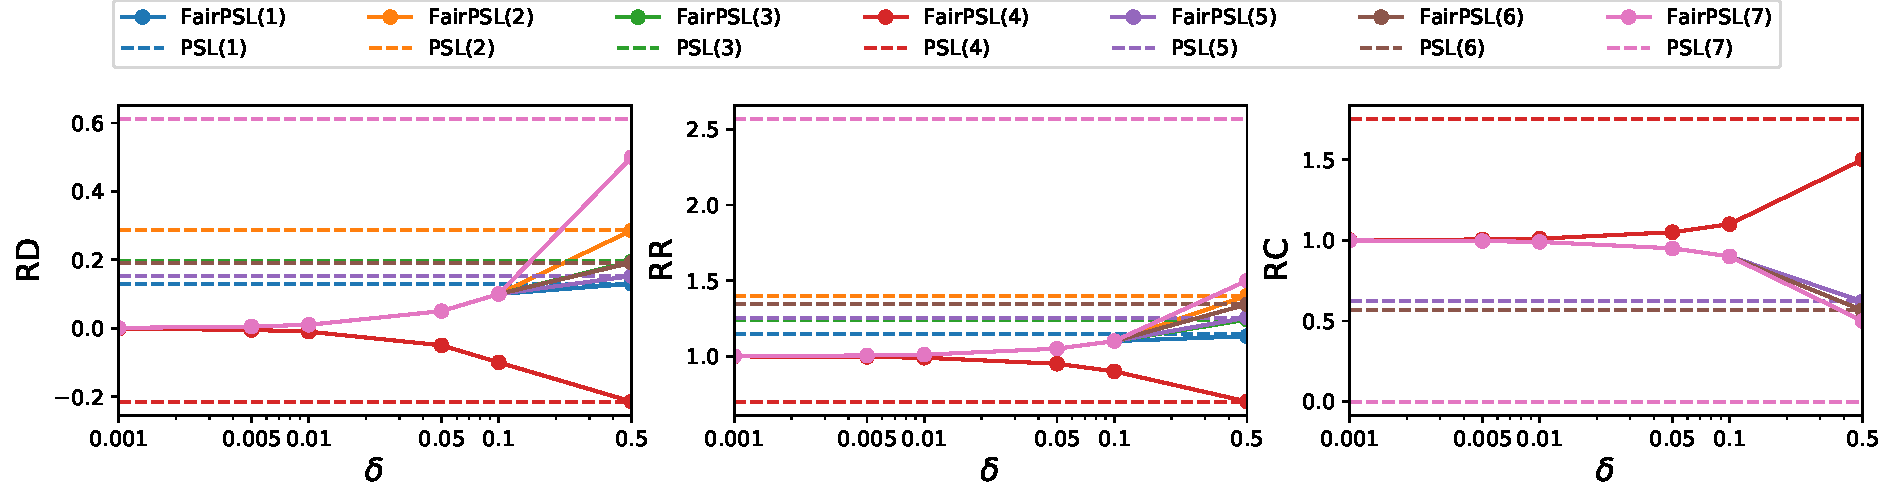
\includegraphics[width=1\linewidth]{figs/results_vis_uni_params.pdf}
\caption{\small Fairness score of predictions obtained by MAP inference of PSL and FairPSL, according to the fairness measures \emph{RD}, \emph{RR}, and \emph{RC}. The labels of datasets are mentioned with parenthesis next to the inference method. The FairPSL values of each measure are obtained by adding the $\delta$-fairness constraint of that measure.\label{fig:results}
}  
\end{figure}

To answer \textbf{Q1}, we run the MAP inference algorithm of PSL and FairPSL on seven synthetic datasets. 
We run the MAP inference of FairPSL multiple times on each dataset: For each of the three fairness measures, we add the corresponding $\delta$-fairness constraint with five thresholds $\{0.001, 0.005, 0.01, 0.05, 0.1, 0.5\}$.

Figure~\ref{fig:results} shows the fairness score of predictions in terms of the three fairness measures. As expected, tighter $\delta$-fairness constraints lead to better scores. Note that the best possible score according to RD is 0, as it computes a difference. Since RR and RC compute ratios, the best possible score according to these measures is 1. In our experiments, with any of these measures, taking $\delta = 0.001$ pushes the score of predictions to its limit.  

The $\delta$-fairness constraints modify the optimization problem of MAP inference by reducing the feasible region to solutions that conform with fairness guarantees. Research question \textbf{Q2} is concerned with the effect of this reduction on the accuracy of predictions. Note that decision quality is the same as the accuracy of predictions. To answer this question, we compare the inferred values for the decision atoms \textit{ToPromote(e)} against their actual values. These values are extracted from the known values of \textit{IsQualified(e)} according to rules 11 and 12 in Table~\ref{tab:pslmodel}. Figure~\ref{fig:accuracy} shows the area under the curve of the receiver operating characteristic~(AUC) of predicting the decision variable in three groups, namely the protected group, the unprotected group (i.e., promotion of the employees who have in-group managers), and all employees. By doing so, we make sure that our fairness constraints do not propagate bias towards either of the populations. Since the results of FairPSL with $\delta$-fairness constraints RR and RC are very similar to the results of RD, we only report the latter here.


\begin{figure}
    \centering
    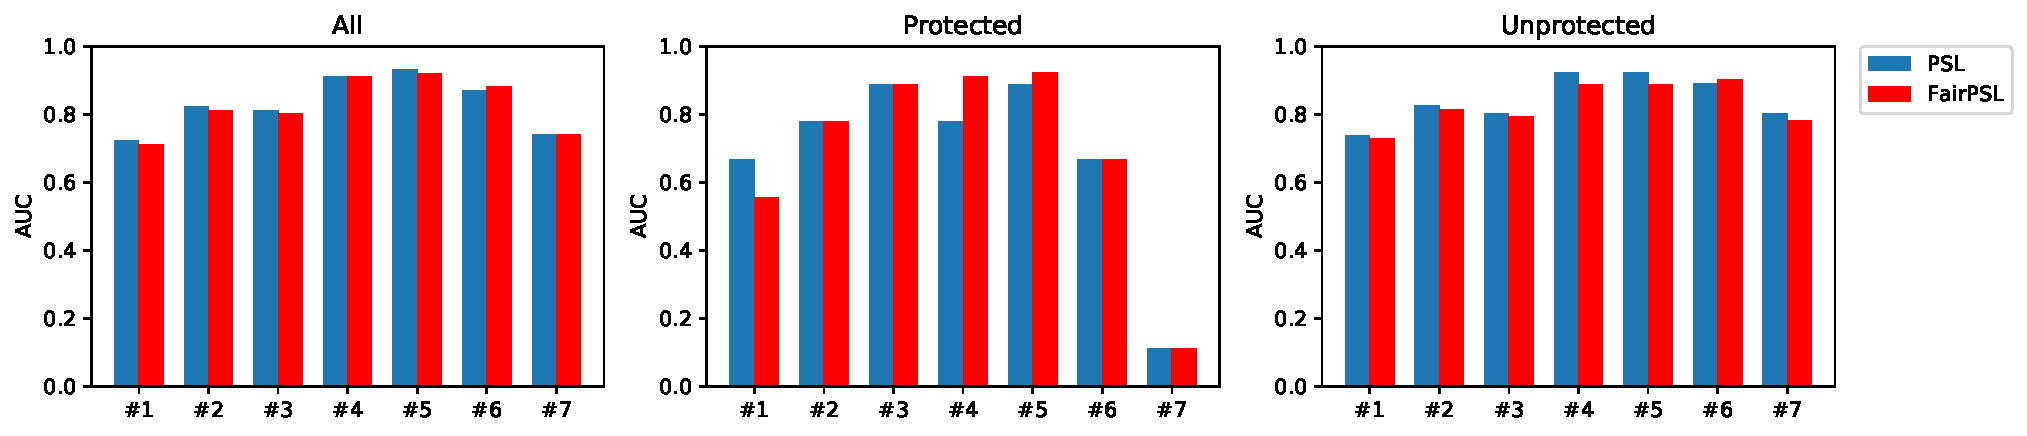
\includegraphics[width=\textwidth]{figs/roc.pdf}
    \caption{\small AUC score of predictions for truth values of unknown atoms \textit{ToPromote(e)} using MAP inference of PSL and FairPSL with $\delta$-fairness constraints $RD$ with $\delta=0.001$.}
    \label{fig:accuracy}
\end{figure}

According to Figure~\ref{fig:accuracy}, the results of both PSL and FairPSL in all seven datasets are close to each other. Note that although fairness may impose a cost in terms of overall accuracy, FairPSL often improves the accuracy of the protected class. Sometimes the overall predictions of FairPSL are even slightly better than PSL (e.g., dataset 6 and 7). As expected, the accuracy of the fourth setting where the opinions are unbiased are similar in both PSL and FairPSL. We observe that prediction of MAP inference for both FairPSL and PSL are similar, thus, in these settings at least, FairPSL guarantees fairness without hurting accuracy. Further investigation is required on the effect of the various ranges of discrimination (i.e., $\theta_1$, $\theta_2$, $\theta_3$, $\theta_4$) on the prediction results of FairPSL.



We also generate various types of organizations in which labels are not uniformly distributed, e.g., one population only occurs at the bottom levels of an organization. While we did not observe any differences in the behavior of our method with respect to accuracy and fairness measure, we found that the degree of discrimination is higher in such organizations. Further investigations on the structure of an organization on discrimination is an interesting direction for future research. 

\section{Conclusion and Future Directions}
\label{sec:conclusion}
Many applications of AI and machine learning affect peoples' lives in important ways. While there is a growing body of work on fairness in AI and ML, it assumes an individualistic notion of fairness.   In this paper, we have proposed a general framework for relational fairness which includes both a rich language for defining discrimination patterns and an efficient algorithm for performing inference subject to fairness constraints. We show our approach enforces fairness guarantees while preserving the accuracy of the predictions. 

There are many avenues for expanding on this work. For example, here we assumed that the discriminative pattern is given, however an automatic mechanism to extract discriminatory situations hidden in a large amount of decision records is an important and required task. Discrimination discovery has been studied for attribute-based fairness~\cite{pedreschi2013discovery}. An interesting next step is discrimination pattern discovery in relational data.

\section*{Acknowledgements}
This work is supported by the National Science Foundation under Grant Numbers CCF-1740850 and IIS-1703331. Golnoosh Farnadi and Behrouz Babaki are  supported by postdoctoral scholarships from IVADO through the Canada First Research Excellence Fund (CFREF) grant.

\begin{thebibliography}{10}
\itemsep=1pt 
\begin{small}

\bibitem{EUlaw}
European union legislation. (a) racial equality directive, 2000; (b) employment
  equality directive, 2000; (c) gender employment directive, 2006; (d) equal
  treatment directive (proposal), 2008.

\bibitem{UKlaw}
{UK} legislation. (a) sex discrimination act, 1975, (b) race relation act,
  1976.

\bibitem{USlaw}
United nations legislation. (a) universal declaration of human rights, 1948,
  (c) convention on the elimination of all forms of racial discrimination,
  1966, (d) convention on the elimination of all forms of discrimination
  against women, 1979.

\bibitem{alshukaili:iswc16}
Duhai Alshukaili, Alvaro A.~A. Fernandes, and Norman~W. Paton.
\newblock Structuring linked data search results using probabilistic soft
  logic.
\newblock In {\em International Semantic Web Conference {(1)}}, volume 9981 of
  {\em Lecture Notes in Computer Science}, pages 3--19, 2016.

\bibitem{bach:jmlr17}
Stephen~H. Bach, Matthias Broecheler, Bert Huang, and Lise Getoor.
\newblock Hinge-loss markov random fields and probabilistic soft logic.
\newblock {\em Journal of Machine Learning Research}, 18:109:1--109:67, 2017.

\bibitem{barocas2016big2}
Solon Barocas and Andrew~D Selbst.
\newblock Big data's disparate impact.
\newblock {\em California Law Review}, 104:671, 2016.

\bibitem{boyd2014networked}
Danah Boyd, Karen Levy, and Alice Marwick.
\newblock The networked nature of algorithmic discrimination.
\newblock In {\em Data and discrimination: Collected essays}, pages 53--57.
  2014.

\bibitem{brewer1979group}
Marilynn~B Brewer.
\newblock In-group bias in the minimal intergroup situation: A
  cognitive-motivational analysis.
\newblock {\em Psychological bulletin}, 86(2):307, 1979.

\bibitem{brewer2007social}
Marilynn~B Brewer.
\newblock The social psychology of intergroup relations: Social categorization,
  ingroup bias, and outgroup prejudice.
\newblock {\em Social Psychology: Handbook of Basic Principles}, 2007.

\bibitem{chouldechova2017fair2}
Alexandra Chouldechova.
\newblock Fair prediction with disparate impact: {A} study of bias in
  recidivism prediction instruments.
\newblock {\em CoRR}, abs/1703.00056, 2017.

\bibitem{dwork2012fairness3}
Cynthia Dwork, Moritz Hardt, Toniann Pitassi, Omer Reingold, and Richard~S.
  Zemel.
\newblock Fairness through awareness.
\newblock In {\em {ITCS}}, pages 214--226. {ACM}, 2012.

\bibitem{ebrahimi:emnlp16}
Javid Ebrahimi, Dejing Dou, and Daniel Lowd.
\newblock Weakly supervised tweet stance classification by relational
  bootstrapping.
\newblock In {\em {EMNLP}}, pages 1012--1017. The Association for Computational
  Linguistics, 2016.

\bibitem{farnadi2018fairness}
Golnoosh Farnadi, Behrouz Babaki, and Lise Getoor.
\newblock Fairness in relational domains.
\newblock In {\em AAAI/ACM Conference on AI, Ethics, and Society (AIES)}, pages
  108--114. ACM, 2018.

\bibitem{feldman2015certifying2}
Michael Feldman, Sorelle~A. Friedler, John Moeller, Carlos Scheidegger, and
  Suresh Venkatasubramanian.
\newblock Certifying and removing disparate impact.
\newblock In {\em {KDD}}, pages 259--268. {ACM}, 2015.

\bibitem{getoor2007introduction}
Lise Getoor and Ben Taskar.
\newblock {\em {Introduction to Statistical Relational Learning}}.
\newblock MIT press Cambridge, 2007.

\bibitem{hardt2016equality3}
Moritz Hardt, Eric Price, and Nati Srebro.
\newblock Equality of opportunity in supervised learning.
\newblock In {\em {NIPS}}, pages 3315--3323, 2016.

\bibitem{kamishima2011fairness}
Toshihiro Kamishima, Shotaro Akaho, and Jun Sakuma.
\newblock Fairness-aware learning through regularization approach.
\newblock In {\em ICDMW}, pages 643--650. {IEEE} Computer Society, 2011.

\bibitem{kouki:recsys15}
Pigi Kouki, Shobeir Fakhraei, James~R. Foulds, Magdalini Eirinaki, and Lise
  Getoor.
\newblock Hyper: {A} flexible and extensible probabilistic framework for hybrid
  recommender systems.
\newblock In {\em RecSys}, pages 99--106. {ACM}, 2015.

\bibitem{counterfactualfairness}
Matt~J. Kusner, Joshua~R. Loftus, Chris Russell, and Ricardo Silva.
\newblock Counterfactual fairness.
\newblock In {\em {NIPS}}, pages 4069--4079, 2017.

\bibitem{Pedreschi:2012}
Dino Pedreschi, Salvatore Ruggieri, and Franco Turini.
\newblock A study of top-k measures for discrimination discovery.
\newblock In {\em {SAC}}, pages 126--131. {ACM}, 2012.

\bibitem{pedreschi2013discovery}
Dino Pedreschi, Salvatore Ruggieri, and Franco Turini.
\newblock The discovery of discrimination.
\newblock In {\em Discrimination and Privacy in the Information Society},
  volume~3 of {\em Studies in Applied Philosophy, Epistemology and Rational
  Ethics}, pages 91--108. Springer, 2013.

\bibitem{ridgeway2004unpacking}
Cecilia~L Ridgeway and Shelley~J Correll.
\newblock Unpacking the gender system: A theoretical perspective on gender
  beliefs and social relations.
\newblock {\em Gender \& society}, 18(4):510--531, 2004.

\bibitem{sridhar:bioinformatics16}
Dhanya Sridhar, Shobeir Fakhraei, and Lise Getoor.
\newblock A probabilistic approach for collective similarity-based drug-drug
  interaction prediction.
\newblock {\em Bioinformatics}, 32(20):3175--3182, 2016.

\bibitem{verma2018fairness2}
Sahil Verma and Julia Rubin.
\newblock Fairness definitions explained.
\newblock In {\em 2018 IEEE/ACM International Workshop on Software Fairness
  (FairWare)}, pages 1--7. IEEE, 2018.

\bibitem{west2014exploiting}
Robert West, Hristo~S. Paskov, Jure Leskovec, and Christopher Potts.
\newblock Exploiting social network structure for person-to-person sentiment
  analysis.
\newblock {\em {TACL}}, 2:297--310, 2014.

\bibitem{zafar2017parity}
Muhammad~Bilal Zafar, Isabel Valera, Manuel Gomez{-}Rodriguez, Krishna~P.
  Gummadi, and Adrian Weller.
\newblock From parity to preference-based notions of fairness in
  classification.
\newblock In {\em {NIPS}}, pages 228--238, 2017.

\bibitem{zemel2013learning}
Richard~S. Zemel, Yu~Wu, Kevin Swersky, Toniann Pitassi, and Cynthia Dwork.
\newblock Learning fair representations.
\newblock In {\em {ICML} {(3)}}, volume~28 of {\em {JMLR} Workshop and
  Conference Proceedings}, pages 325--333. JMLR.org, 2013.

\end{small}
\end{thebibliography}

\end{document}

\end{article}

\iffalse

\begin{article}
{{ProvDB:} Provenance-enabled Lifecycle Management of Collaborative Data Analysis Workflows}
{Hui Miao, Amol Deshpande}
\graphicspath{{submissions/ProvDB/figs/}}
%\documentclass[11pt,dvipdfm]{article}
\documentclass[11pt]{article}
\usepackage{deauthor,times,graphicx} %required
\usepackage{amsmath,amssymb}
\usepackage{multirow}
\usepackage{algorithm}
\usepackage{algpseudocode}
\usepackage{todonotes}
\usepackage{url}

% \graphicspath{{farnadi/}}

\newtheorem{mydef}{\textbf{Definition}}
\newtheorem{myex}{\textbf{Example}}
\newtheorem{mytheorem}{\textbf{Theorem}}


\begin{document}

\title{A Declarative Approach to Fairness in Relational Domains}
\author{Golnoosh Farnadi$^{1,2}$, Behrouz Babaki$^1$, Lise Getoor$^3$\\
$^1$Polytechnique Montr\'{e}al, $^2$ Mila, $^3$ UC Santa Cruz \\
farnadig@mila.quebec, behrouz.babaki@polymtl.ca, getoor@soe.ucsc.edu}

\maketitle

\begin{abstract}
AI and machine learning tools are being used with increasing frequency for decision making in domains that affect peoples' lives such as employment, education, policing and %loan approval
financial qualifications. These uses raise concerns about biases of algorithmic discrimination and have motivated the development of fairness-aware machine learning. However, existing fairness approaches are based solely on attributes of individuals. In many cases, discrimination is much more complex, and taking into account the social, organizational, and other connections between individuals is important. We introduce new notions of fairness that are able to capture the relational structure in a domain. We use first-order logic to provide a flexible and expressive language for specifying complex relational patterns of discrimination. Furthermore, we extend an existing statistical relational learning framework, probabilistic soft logic~(PSL), to incorporate our definition of relational fairness. We refer to this fairness-aware framework FairPSL. FairPSL makes use of the logical definitions of fairnesss but also supports a probabilistic interpretation. In particular, we show how to perform maximum a posteriori~(MAP) inference by exploiting probabilistic dependencies within the domain while avoiding violations of fairness guarantees. Preliminary empirical evaluation shows that we are able to make both accurate and fair decisions.
\end{abstract}

\section{Introduction}
\label{sec:introduction}

Over the past few years, AI and machine learning have become essential components in operations that drive the modern society, e.g., in financial, administrative, and educational spheres. \emph{Discrimination} happens when qualities of individuals which are not relevant to the decision making process influence the decision. Delegating decision making to an automated process raises questions about discriminating against individuals with certain traits based on biases in the data. This is especially important when the decisions have the potential to impact the lives of individuals, for example, the decisions on granting loans, assigning credit, and employment. 

\emph{Fairness} is defined as the absence of discrimination in a decision making process. The goal of \emph{fairness-aware} machine learning is to ensure that the decisions made by an algorithm do not discriminate against a population of individuals~\cite{feldman2015certifying2,boyd2014networked,hardt2016equality3}. Fairness has been well studied in the social sciences and legal scholarship (for an in-depth review see~\cite{barocas2016big2}), and there is emerging work on fairness-aware ML within the AI and computer science communities. For example, fairness through awareness/Lipschitz property~\cite{dwork2012fairness3}, individual fairness~\cite{zemel2013learning}, statistical parity/group fairness~\cite{kamishima2011fairness}, counterfactual fairness~\cite{counterfactualfairness}, demographic parity/disparate impact~\cite{feldman2015certifying2,chouldechova2017fair2}, preference-based fairness~\cite{zafar2017parity}, and equality of opportunity~\cite{hardt2016equality3}.

The existing work in fairness-aware machine learning is based on a definition of discrimination where a decision is influenced by an \emph{attribute} of an individual. An attribute value upon which discrimination is based (such as gender, race, or religion) is called a \emph{sensitive attribute}. The sensitive attribute defines a population of vulnerable individuals known as the \emph{protected group}. A fair decision-making process treats the protected group the same as the \emph{unprotected group}. 

However, in many social contexts, discrimination is the result of complex interactions and can not be described solely in terms of attributes of an individual. For example, consider an imaginary scenario in an organization in which younger female workers who have older male supervisors have lower chances of promotion than their male counterparts.\footnote{Of course, many other patterns may be possible: female bosses may promote female subordinates and discriminate against male workers, or male bosses may promote female employees.  Our goal is to provide a general framework which is able to describe arbitrarily complex discrimination patterns.} 
 This discrimination pattern involves two attributes of the individual (gender and age), a relationship with another individual (supervisor), and two attributes of the second individual. Addressing such complex cases poses two challenges. First, the concepts of discrimination and fairness need to be extended to capture not only attributes of individuals but also the relationships between them. Second, a process is required that ensures that fair decisions are made about individuals who are affected by such patterns. In this paper we address both of these challenges.
We use first-order logic (FOL) to extend the notion of fairness to the relational setting. FOL is an expressive representation for relational problems which is also widely used for learning in relational domains. Moreover, we extend an existing framework for statistical relational learning~\cite{getoor2007introduction} called probabilistic soft logic (PSL)\footnote{http://psl.linqs.org/}~\cite{bach:jmlr17}. PSL combines logic and probability for learning and reasoning over uncertain relational domains. One of the most common reasoning tasks in PSL is called maximum a posteriori (MAP) inference, which is performed by finding the most probable truth values for unknowns over a set of given evidence. We develop a new MAP inference algorithm which is able to maximize the a posteriori values of unknown variables \emph{subject to} fairness guarantees. An early version of this paper which this work builds upon and extends appeared in~\cite{farnadi2018fairness}.

\looseness-1
Our contributions are as follows: 1) we propose fairness-aware machine learning for the relational setting; 2) we extend PSL into a fairness-aware framework called FairPSL which can represent the logical definition of fairness; 3) we develop a new MAP inference algorithm which is able to maximize the posteriori values of unknown variables \emph{subject to} fairness guarantees; 4) we empirically evaluate our proposed framework on synthetic data. 

\section{Motivation}
\label{sec:motivation}

Discrimination in social contexts have been studied in the field of social psychology~\cite{brewer2007social,brewer1979group,ridgeway2004unpacking}. There is a large literature on various aspects of relational bias in social contexts such as \emph{in-group-out-group bias}, \emph{gender bias}, and \emph{ethnicity-based favoritism} that can result in discrimination. 
As an example, consider gender bias in the workplace that reflects stereotypically masculine criteria and male-based favoritism. Such gender bias 
typically places women in lower positions and negatively impacts their opportunities. Further, lack of women in leadership positions may affect the promotion of women and results in a glass ceiling that keeps women from rising beyond a certain level in the hierarchy. This scenario shows that considering  protected attributes such as gender is not always sufficient to detect the source of bias and avoid discrimination, one also has to consider the relational information, in this case the organization hierarchy. Note that this can be generalized to any ingroup/outgroup scenario where the sensitive attribute could be race, religion, age, marital-status, etc.

The existing work on designing fair algorithms in machine learning exclusively focuses on \emph{attribute-based fairness}, which is based on the following assumptions: First, there is an assumption that the individuals (sometimes referred to as units or entities) are independent and described by simple attribute vectors. Second, the group for which one wishes to ensure fairness (known as the \emph{protected group}) is defined on the basis of some attribute values. Finally, there is a decision that is associated with each individual, and the goal is to ensure that members of the protected group are subject to a fair decision (we discuss different fairness measures in Section~\ref{sec:fairnessmeasure}).  We illustrate  attribute-based fairness in the following example. 

\begin{myex}[Loan Processing]
\label{ex:loan}
A bank bases its decisions about granting a loan on attributes of the applicant. The goal is to decide whether to grant a loan to an applicant using a predictive model. The bank needs to ensure that the obey fair lending practices and ensure that gender, race, sexual orientation of applicants has no influence on the decision. In this scenario, the protected group is the historically disadvantaged applicants.  
\end{myex}
The current fairness-aware machine learning techniques are not capable of modeling relations and hence cannot be used to make the decision making model fair. However, in many decision making scenarios, especially in social and organizational settings, the domain is relational, and the protected group itself might be best represented using a relational definition. We illustrate this setting in the following scenario:
\begin{myex}[Performance Review]
\label{ex:review}
Consider an organization where decisions about the promotion of employees is based on two criteria: 1) an objective performance measure, and 2) the opinion of their direct and indirect managers above them. The opinions are inferred from the performance reviews which are collected periodically. Not every manager can submit a review for all its subordinates, this is especially the case for top-level managers who have a large number of subordinates. Hence, the opinions of managers are collectively inferred from the opinions of their sub-ordinates. However, some employees may be biased, and judge other employees unfavorably, by favoring employees who are similar to themselves (same gender, race, religion, etc.) over employees who are dissimilar. The organization needs to ensure that promotion of employees do not have any relational bias caused by in-group-out-group favoritism.

\end{myex}
Example~\ref{ex:review} describes a prediction problem over a database that consists of relations between employees. Such prediction tasks are best handled by techniques from the relational learning domain. To ensure fair prediction in such settings, we need to extend the notion of \emph{attribute-based fairness} to \emph{relational fairness}. Throughout this paper, we use the performance review problem as a running example for relational fairness.

\section{Fairness Formalism}
\label{sec:formulation}

A representation that can describe different types of entities and different relationships between them is called relational. In this section, we use first-order logic to define relational fairness. We employ first-order logic as an expressive representation formalism which can represent objects and complex relationships between them. We start by defining an atom:

\begin{mydef}[Atom]
An atom is an expression of the form $P(a_1, a_2, \ldots, a_n)$ where each argument $a_1, a_2,$ $\ldots,$ $a_n$ is either a constant or a variable. The finite set of all possible substitutions of a variable to a constant for a particular variable $a$ is called its \textit{domain} $D_{a}$. If all variables in $P(a_1, a_2, \ldots, a_n)$ are substituted by some constant from their respective domain, then we call the resulting atom a \textit{ground atom}. 
\end{mydef}

\begin{myex}
In our loan processing problem (Example~\ref{ex:loan}), we can represent applicants' attributes by atoms. For instance, atom $Female(v)$ indicates whether or not applicant $v$ is female. Similarly, we can represent relations with atoms. In the performance review problem in Example~\ref{ex:review} the atom $Manager(m,e)$ indicates whether or not employee $m$ is a direct or indirect manager of employee $e$.
\end{myex}

The relational setting provides the flexibility to express complex definitions with formulae.

\begin{mydef}[Formula] 
A formula is defined by induction: every atom is a formula. If $\alpha$ and $\beta$ are formulae, then $\alpha \vee \beta$, $\alpha \wedge \beta$, $\neg \alpha$, $\alpha \rightarrow \beta$ are formulae. If $x$ is a variable and $\alpha$ is a formula, then the quantified expressions of the form $\exists x$ $\alpha$ and $\forall x$ $\alpha$ are formulae.    
\end{mydef}

To characterize groups of individuals based on a formula, we define the notion of \emph{population}.

\begin{mydef}[Population]
We denote formula $F$ which has only one free variable $v$ (i.e., other variables in $F$ are quantified) by $F[v]$. The population defined by $F[v]$ is the set of substitutions of $v$ for which $F[v]$ holds.   
\end{mydef}


\begin{myex}
\label{ex:disformula}
Consider the formula $F[v] := \forall u, \, \textit{Manager}(u,v) \rightarrow \neg \textit{SameGroup}(u, v)$. The population specified by this formula is the set of individuals all of whose managers belong to a group different from theirs. 
\end{myex}

The truth value of a formula is derived from the truth value of atoms that it comprises, according to the rules of logic. Each possible assignment of truth values to ground atoms is called an \emph{interpretation}. 


\begin{mydef}[Interpretation]
An interpretation $I$ is a mapping that associates a truth value $I(P)$ to each ground atom $P$. For Boolean truth values, $I$ associates true to 1 and false to 0 truth values. For soft logic (see Definition~\ref{def:softlogic}) $I$ maps each ground atom $P$ to a truth value in interval $[0, 1]$.
\end{mydef}

In attribute-based fairness, it is assumed that there is a certain attribute of individuals, i.e, the sensitive attribute,  that we do not want to affect a decision. Gender, race, religion and marital status are examples of sensitive attributes. Discrimination has been defined in social science studies as a treatment in favor or against a group of individuals given their sensitive attribute. This group of individuals is the protected group. 

In a relational setting, both the sensitive attributes of an individual and their participation in various relations may have an undesired effect on the final decision. We characterize the protected group in a relational setting by means of a population. In practice, we are often interested in maintaining fairness for a specific population such as applicants, students, employees, etc. This population is then partitioned into the protected and unprotected groups. We define a \emph{discriminative pattern} which is a pair of formulae to capture these groups: 1) $F_1[v]$: to specify the difference between the protected and unprotected groups and 2) $F_2[v]$: to specify the population over which we want to maintain fairness. 

\begin{mydef}[Discriminative pattern]
A discriminative pattern is a pair $\textit{DP}[v]:=(F_1[v], F_2[v])$ , where $F_1[v]$ and $F_2[v]$ are formulae.
\end{mydef}

\begin{myex}
\label{ex:pattern}
The two formulae in the discrimination pattern $\textit{DP}[v]:= \big((\forall u, \,  \textit{Manager}(u,v) \rightarrow  \neg \textit{SameGroup}(u, v)),$ $\textit{Employee}(v)\big)$ specify two populations, namely all employees and those employees who belong to a group different from their managers.
\end{myex}

Given the definition of the discriminative pattern, we have a rich language to define the scope of the protected and unprotected groups in a relational setting.

\begin{mydef}[Protected group] Given an interpretation $I$, the protected group is a population of the form:
{$$PG :=\{ v : F_1[v] \wedge F_2[v]\}$$}
which is defined as the set of all instances hold for variable $v$ for which $F_1[v] \wedge F_2[v]$ is true under interpretation $I$, that is, $I(F_1[v] \wedge F_2[v]) = 1$. 
Similarly, the \emph{unprotected group} is a population of the form: 
{$$UG := \{ v : \neg F_1[v] \wedge  F_2[v]\}$$}
which is defined as the set of all instances hold for variable $v$ 
for which $I(\neg F_1[v] \wedge F_2[v]) = 1$. 
\end{mydef}

\begin{myex}
The protected group of the discrimination pattern specified in Example~\ref{ex:pattern} is {$PG := \big\{ v : \big(\forall u, \,$ $ \textit{Manager}(u, v) \rightarrow \neg \textit{SameGroup}(u, v)\big) \wedge \textit{Employee}(v) \big\}$} and the unprotected group is {$UG :=  \big\{ v:  \big(\exists u, \, \textit{Manager}(u,v) \wedge \textit{SameGroup}(u, v)\big) \wedge \textit{Employee}(v) \big\}$}. This means our protected group is the set of employees belonging to a group different from their managers,
and our unprotected group consists of other employees. 
\end{myex}

Discrimination is defined in terms of a treatment or decision that distinguishes between the protected and unprotected groups. Here we define the \emph{decision} atom.
\begin{mydef}[Decision atom] A decision atom $d(v)$ is an atom containing exactly one variable $v$ that specifies a decision affecting the protected group which is defined either by law or end-user.
\end{mydef}
\begin{myex}
The decision atom ${\textit ToPromote}(v)$ indicates whether or not $v$ receives a promotion.
\end{myex}

Note that the fairness formulation in this section is designed for the relational setting, however relational fairness subsumes the attribute-based fairness such that: a sensitive attribute is defined by an atom with one argument and $F_2[v]$ in discrimination pattern is $\textit{Applicant}(v)$. For example, discrimination pattern of our loan processing problem in Example~\ref{ex:loan} is of the form $\textit{DP} := ( \textit{Female}(v), \textit{Applicant}(v))$ that denotes female applicants as the protected group (i.e., $PG :=  \{ v: \textit{Female}(v) \}$) and male applicants as the unprotected group (i.e., $UG := \{ v: \neg \textit{Female}(v)\}$).


\section{Fairness Measures}
\label{sec:fairnessmeasure}

Over the past few years, many fairness measures have been introduced~\cite{verma2018fairness2}. An important class of these measures are \emph{group fairness} measures which quantify the inequality between different subgroups. Some of the most popular measures in this class include \emph{equal opportunity}, \emph{equalized odds}, and \emph{demographic parity}~\cite{hardt2016equality3}. In this paper we restrict our focus to the latter. In an attribute-value setting, demographic parity means that the decision should be independent of the protected attributes. Assume that binary variables $A$ and $C$ denote the decision and protected attributes, and the preferred value of $A$ is one. Demographic parity requires that:

\begin{equation*}
    P(A=1 | C=0) = P(A=1 | C=1)
\end{equation*}

We will now generalize this measure to the relational setting using the notations defined in Section~\ref{sec:formulation}. Let $a$ and $c$ denote the counts of denial (i.e., negative decisions) for protected and unprotected groups, and $n_{1}$ and $n_{2}$ denote their sizes, respectively. Given the decision atom $d(v)$, discriminative pattern $\textit{DP}(F_1[v], F_2[v])$, and interpretation $I$, these counts are computed by the following equations: 
{
\begin{flalign}
    & a \equiv \sum_{v \in D_v} I\big( \neg d(v) \wedge  F_1[v] \wedge F_2[v]) \label{eq:a}\\
    & c \equiv \sum_{v \in D_v} I\big( \neg d(v) \wedge  \neg F_1[v] \wedge  F_2[v]) \label{eq:c}\\
    & n_{1} \equiv \sum_{v \in D_v} I\big(F_1[v] \wedge F_2[v]) \label{eq:n1}\\
    & n_{2} \equiv \sum_{v \in D_v} I\big(\neg F_1[v] \wedge  F_2[v]) \label{eq:n2}
\end{flalign}}
The proportions of denying for protected and unprotected groups are $p_1 = \frac{a}{n_1}$ and $p_2 = \frac{c}{n_2}$, respectively. There are a number of data-driven measures~\cite{Pedreschi:2012} which quantify demographic disparity and can be defined in terms of $p_1$ and $p_2$:
\begin{itemize}
    \item \textbf{Risk difference}: $RD = p_1 - p_2$, also known as absolute risk reduction. 
    \item \textbf{Risk Ratio}: $RR = \frac{p_1}{p_2}$, also known as relative risk. 
    \item \textbf{Relative Chance}: $RC = \frac{1 - p_1}{1 - p_2}$ also, known as selection rate.
\end{itemize}
These measures have been used in the legal systems of European Union, UK, and US~\cite{EUlaw,UKlaw,USlaw}. Notice that RR is the ratio of the proportion of benefit denial between the protected and unprotected groups, while RC is the ratio of the proportion of benefit granted. Finally, we introduce the notion of $\delta$-fairness.

\begin{mydef}[$\delta$-fairness]
If a fairness measure for a decision making process falls within some $\delta$-window, then the process is \emph{$\delta\text{-fair}$}. Given $0 \leq \delta \leq 1$, the  $\delta$-windows for measures RD/RR/RC are defined as:
{\begin{flalign*}
	     - \delta \leq &RD \leq \delta \\
	     1- \delta \leq &RR \leq 1+ \delta\\
	     1- \delta \leq &RC \leq 1+ \delta
	\end{flalign*}}
\end{mydef}

To overcome the limitations of attribute-based fairness, we introduce a new statistical relational learning~(SRL) framework~\cite{getoor2007introduction} suitable for modelling fairness in relational domain. In the next section, we review probabilistic soft logic~(PSL). We then extend PSL with the definition of relational fairness introduced above in Section~\ref{sec:fairMAP}. Our fairness-aware framework, ``FairPSL'', is the first SRL framework that performs fair inference. 

\section{Background: Probabilistic Soft Logic}
\label{sec:psl}

In this section, we review the syntax and semantics of PSL, and in the next section we extend MAP inference in PSL with fairness constraints to define MAP inference in FairPSL.

PSL is a probabilistic programming language for defining hinge-loss Markov random fields~\cite{bach:jmlr17}. Unlike other SRL frameworks whose atoms are Boolean, atoms in PSL can take continuous values in the interval $[0,1]$. PSL is an expressive modeling language that can incorporate domain knowledge with first-order logical rules and has been used successfully in various domains, including bioinformatics~\cite{sridhar:bioinformatics16}, recommender systems~\cite{kouki:recsys15}, natural language processing~\cite{ebrahimi:emnlp16}, information retrieval~\cite{alshukaili:iswc16}, and social network analysis~\cite{west2014exploiting}, among many others. 
 
A PSL model is defined by a set of first-order logical rules called \emph{PSL rules}.

\begin{mydef} [PSL rule] a PSL rule $r$ is an expression of the form:
{\begin{equation}
\lambda_{r}: T_1 \land T_2 \land \ldots \land T_w \rightarrow H_1 \vee H_2 \vee \ldots \vee H_l
\end{equation}}

where { $T_1, T_2, \ldots, T_w, H_1, H_2, \ldots, H_l$} are atoms or negated atoms and { $\lambda_{r} \in \mathbb{R}^{+} \cup \infty$} is the weight of the rule $r$.  We call { $T_1 \land T_2 \land \ldots \land T_w$} the body of $r$ ($r_{body}$), and { $H_1 \vee H_2 \vee \ldots \vee H_l$} the head of $r$ ($r_{head}$).
\end{mydef}


Since atoms in PSL take on continuous values in the unit interval $[0,1]$, next we define soft logic to calculate the value of the PSL rules under an interpretation $I$.

\begin{mydef}[Soft logic]
\label{def:softlogic}
The ({$\tilde{\wedge}$}) and ({$\tilde{\vee}$}) and negation ({$\tilde{\neg}$}) are defined as follows. For {$m, n \in [0,1]$} we have: {$m \tilde{\wedge} n = \max(m+n -1, 0)$}, {$m \tilde{\vee} n = \min(m+n , 1)$} and {$\tilde{\neg} m = 1 - m$}. The $\, \tilde{} \,$ indicates the relaxation over Boolean values.
\end{mydef}

The probability of truth value assignments in PSL is determined by the rules' \emph{distance to satisfaction}.

\begin{mydef}[The distance to satisfaction]
The distance to satisfaction $d_{r}(I)$ of a rule $r$ under an interpretation $I$ is defined as:
{
\begin{equation}
d_{r}(I) = \max\{0, I(r_{body})-I(r_{head})\}
\end{equation}}
\end{mydef}

By using Definition~\ref{def:softlogic}, one can show that the closer the interpretation of a grounded rule $r$ is to 1, the smaller its distance to satisfaction. A PSL model induces a distribution over interpretations $I$. Let $R$ be the set of all grounded rules, then the probability density function is:
{
\begin{equation}
f(I) ={\frac{1}{Z}} \exp[-\sum_{r\in R} \lambda_{r}(d_{r}(I))^p]
\label{eq:potential}
\end{equation}
}
\noindent where { $\lambda_{r}$} is the weight of rule $r$, {
$Z = \int_{I} \exp[ -\sum_{r\in R} \lambda_{r}(d_{r}(I))^p]$
} is a normalization constant, and { $p \in \{1,2\}$} provides a choice of two different loss functions, $p=1$ (i.e., linear), and $p=2$ (i.e, quadratic). These probabilistic models are instances of hinge-loss Markov random fields~(HL-MRF)~\cite{bach:jmlr17}. The goal of maximum a posteriori (MAP) inference is to find the most probable truth assignments $I_{\textit{MPE}}$ of unknown ground atoms given the evidence which is defined by the interpretation $I$. Let $X$ be all the evidence, i.e., $X$ is the set of ground atoms such that $\forall x \in X, I(x)$ is known, and let $Y$ be the set of ground atoms such that $\forall y \in Y, I(y)$ is unknown. Then we have
{
\begin{equation}
I_{\textit{MAP}}(Y) = \textit{arg}\max_{I(Y)} P(I(Y)|I(X))
\end{equation}}
Maximizing the density function in Equation~\ref{eq:potential} is equivalent to minimizing the weighted sum of the distances to satisfaction of all rules in PSL. 

\begin{table*}[t]
    \centering
    \begin{tabular}{|lll|}
    \hline
    &&\\
    $R1$ & $\lambda_1$ &: $\textit{IsQualified}(e) \rightarrow \textit{HighPerformance}(e)$ \\
    $R2$ & $\lambda_1$ &: $\neg \textit{IsQualified}(e) \rightarrow \neg \textit{HighPerformance}(e)$ \\
    $R3$ & $\infty$ &: $\textit{PositiveReview}(e1, e2) \rightarrow \textit{PositiveOpinion}(e1, e2)$ \\
    $R4$ & $\infty$ &: $\neg \textit{PositiveReview}(e1, e2) \rightarrow \neg \textit{PositiveOpinion}(e1, e2)$ \\
    $R5$ & $\lambda_1$ &: $\textit{PositiveOpinion}(e1, e2) \wedge \textit{Manager}(m, e1) \rightarrow \textit{PositiveOpinion}(m, e2)$ \\
    $R6$ & $\lambda_1$ &: $\neg \textit{PositiveOpinion}(e1, e2) \wedge \textit{Manager}(m, e1) \rightarrow \neg \textit{PositiveOpinion}(m, e2)$ \\
    $R7$ & $\lambda_1$ &: $\textit{PositiveOpinion}(m, e) \wedge \textit{Manager}(m, e) \rightarrow \textit{IsQualified}(e)$ \\
    $R8$ & $\lambda_1$ &: $\neg \textit{PositiveOpinion}(m, e) \wedge \textit{Manager}(m, e) \rightarrow \neg \textit{IsQualified}(e)$ \\
    $R9$ &  $\lambda_1$ &: $\neg \textit{ToPromote}(e)$\\
    $R10$ & $\infty$ &: $\textit{IsQualified}(e) \rightarrow \textit{ToPromote}(e)$ \\
    $R11$ & $\infty$ &: $\neg \textit{IsQualified}(e) \rightarrow \neg \textit{ToPromote}(e)$ \\
    &&\\
    \hline
    \end{tabular}
    \caption{\small A simplified PSL model for the \emph{Performance Reviewing} problem}
    \label{tab:pslmodel}
\end{table*}

\begin{myex}
\label{ex:pslmodel}
The simplified PSL model for the performance reviewing problem in Example\ref{ex:review} is given in Table~\ref{tab:pslmodel}. The goal of MAP inference for this problem is to infer employees to promote. We simplified the model by assigning the same weight to all soft rules (i.e., $\lambda_i= 1$ where $i=\{1,2,5,6,7,8,9\}$). Below we explain the meaning of each rule in the model.

Rule $R1$ indicates that qualified employees have high performance and similarly rule $R2$ expresses that a negative qualification of employees is derived from their low performance. Rules $R5$ and $R6$ presents the propagation of opinion from bottom to top of the organizational hierarchy, i.e., managers have similar opinions towards employees given the opinions of their sub-ordinate managers. And rules $R7$ and $R8$ indicate that the positive/negative opinion of direct/indirect managers derive from the qualification of an employee. Rule $R9$ indicates the prior that not all employees get promoted. We also have four hard constraints (i.e., rules $R3$, $R4$, $R10$ and $R11$) where the weight of the rules are $\infty$. Rules $R3$ and $R4$ indicate that submitted positive/negative reviews should reflect positive/negative opinions. And two rules $R10$ and $R11$ show that a highly qualified employee should get promoted. 
\end{myex}

\section{Fairness-aware PSL (FairPSL)}
\label{sec:fairMAP}

The standard MAP inference in PSL aims at finding values that maximize the conditional probability of unknowns. Once a decision is made according to these values, one can use the fairness measure to quantify the degree of discrimination. A simple way to incorporate fairness in MAP inference is to add the $\delta$-fairness constraints to the corresponding optimization problem.   

Consider risk difference, $\textit{RD}$, where $\textit{RD} \equiv \frac{\mathbf{a}}{n_1} - \frac{\mathbf{c}}{n_2}$. The $\delta$-fairness constraint $-\delta \leq \textit{RD} \leq \delta$ can be encoded as the following constraints:
{\begin{align}
    & n_2 \mathbf{a} - n_1 \mathbf{c} - n_1 n_2 \delta \leq 0 \label{eq:RD1}\\
    & n_2 \mathbf{a} - n_1 \mathbf{c} + n_1 n_2 \delta \geq 0
\end{align}}
Similarly, from $\textit{RR} \equiv \frac{\mathbf{a} / n_1}{\mathbf{c} / n_2}$ and the $\delta$-fairness constraint $1 - \delta \leq \textit{RR} \leq 1 + \delta$ we obtain:
{\begin{align}
    & n_2 \mathbf{a} - (1 + \delta) n_1 \mathbf{c} \leq 0 \\
    & n_2 \mathbf{a} - (1 - \delta) n_1 \mathbf{c} \geq 0
\end{align}}
And finally, $\textit{RC} \equiv \frac{1 - \mathbf{a} / n_1}{1 - \mathbf{c} / n_2}$ and the $\delta$-fairness constraint $1 - \delta \leq \textit{RC} \leq 1 + \delta$ gives:
{ \begin{align}
    & - n_2 \mathbf{a} + (1 + \delta) n_1 \mathbf{c} - \delta n_1 n_2 \leq 0 \\
    & - n_2 \mathbf{a} + (1 - \delta) n_1 \mathbf{c} + \delta n_1 n_2 \geq 0 \label{eq:RC2}
\end{align}}
A primary advantage of PSL over similar frameworks is that its MAP inference task reduces to a convex optimization problem which can be solved in polynomial time. To preserve this advantage, we need to ensure that the problem will remain convex after the addition of $\delta$-fairness constraints. 

\begin{mytheorem}
The following condition is sufficient for preserving the convexity of MAP inference problem after addition of $\delta$-fairness constraints: The formulae $F_1[v]$ and $F_2[v]$ do not contain an atom $y \in Y$ and all atoms in $F_1[v]$ and $F_2[v]$ have values zero or one.
\end{mytheorem}
\begin{proof}
Since $I(F_1[v])$ and $I(F_2[v])$ do not depend on $I(Y)$, the values $n_{1}$ and $n_{2}$ are constants that can be computed in advance. Let us define the sets $D_v^a = \{ v \in D_v : F_1[v] \wedge F_2[v] \, \text{is true} \}$ and $D_v^c = \{ v \in D_v : \neg F_1[v] \wedge F_2[v] \, \text{is true} \}$. Since $F_1[v]$ and $F_2[v]$ can be only zero or one, we can rewrite the equations~\ref{eq:a} and \ref{eq:c} as:
{
\begin{align*}
    & \mathbf{a} = \sum_{v \in D_v^a} I(\neg d(v)) = |D_v^a| - \sum_{v \in D_v^a} I(d(v))\\
    & \mathbf{c} = \sum_{v \in D_v^c} I(\neg d(v)) = |D_v^c| - \sum_{v \in D_v^c} I(d(v))
\end{align*}}
\noindent which indicates that $\mathbf{a}$ and $\mathbf{c}$ can be expressed as linear combinations of variables in the optimization problem. This means that constraints~\ref{eq:RD1}-\ref{eq:RC2} are linear. Hence, addition of these constraints preserves the convexity of the optimization problem. 
\end{proof}

\section{Experiments}
\label{sec:experiment}

\begin{figure}
  \begin{minipage}[c]{0.6\textwidth}
    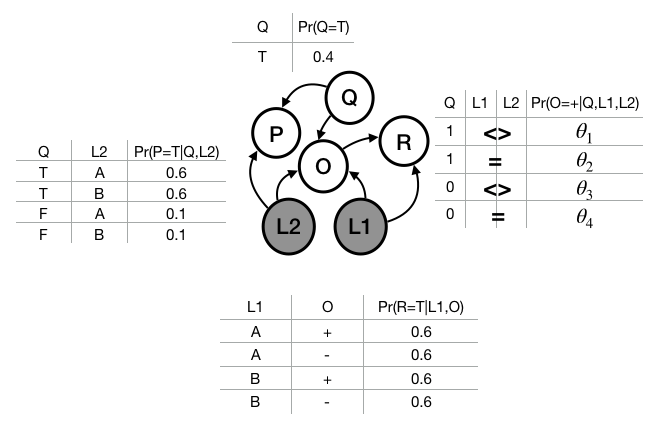
\includegraphics[width=\textwidth]{figs/BN.png}
  \end{minipage}\hfill
  \begin{minipage}[c]{0.45\textwidth}
    \caption{
        \small The model used for generating the datasets. There are four binary random variables, P, Q, O, and R. \textbf{P}: indicates whether or not the employee has high performance; \textbf{Q}: indicates whether or not an employee has high qualification; \textbf{O}: indicates whether or not the colleague submits the positive opinion towards the employee;  \textbf{R}: indicates whether or not the colleague has a positive opinion towards the employee;  \textbf{L1, L2}: indicates the label of the review provider and review receiver (observed).
    } \label{fig:BN}
  \end{minipage}
\end{figure}

We show the effectiveness of FairPSL by performing an empirical evaluation. We investigate two research questions in our experiments:
\begin{description}
\item[Q1] What is the effect of the fairness threshold $\delta$ on the fairness measures $RD/RC/RR$?
\item[Q2] How is decision quality affected by imposing $\delta$-fairness constraints?
\end{description}

Note that although we present the result for specific parameters of the framework in this section, we ran extensive analysis and the results we present are representative. We implemented the MAP inference routines of PSL and FairPSL in Python, using Gurobi-8.1\footnote{\url{www.gurobi.com}} as the backend solver. The FairPSL code, code for the data generator and data is publicly available\footnote{https://github.com/gfarnadi/FairPSL}. 

\subsection{Data generation}
  
We evaluate the FairPSL inference algorithm on synthetic datasets representing the performance review scenario (introduced in Example~\ref{ex:review}). The organization hierarchy is generated synthetically. 
The organization hierarchy generator is parameterized by two numbers: the number of employees in the organization ($n$) and the number of employees managed by each manager ($k$). Each employee is randomly assigned with a label \emph{A} or \emph{B}. An examples organization hierarchy with $n$=50 and $k$=3 is shown in Figure~\ref{fig:hierachy}.

\begin{figure}
  \begin{minipage}[c]{0.3\textwidth}
    \caption{
        \small An example of an organizational hierarchy with five levels and 50 employees with k=3. Each employee either has label A (shown with grey) or B (shown with white).
    }\label{fig:hierachy} 
	\end{minipage} \hfill
    \begin{minipage}[c]{0.7\textwidth}
    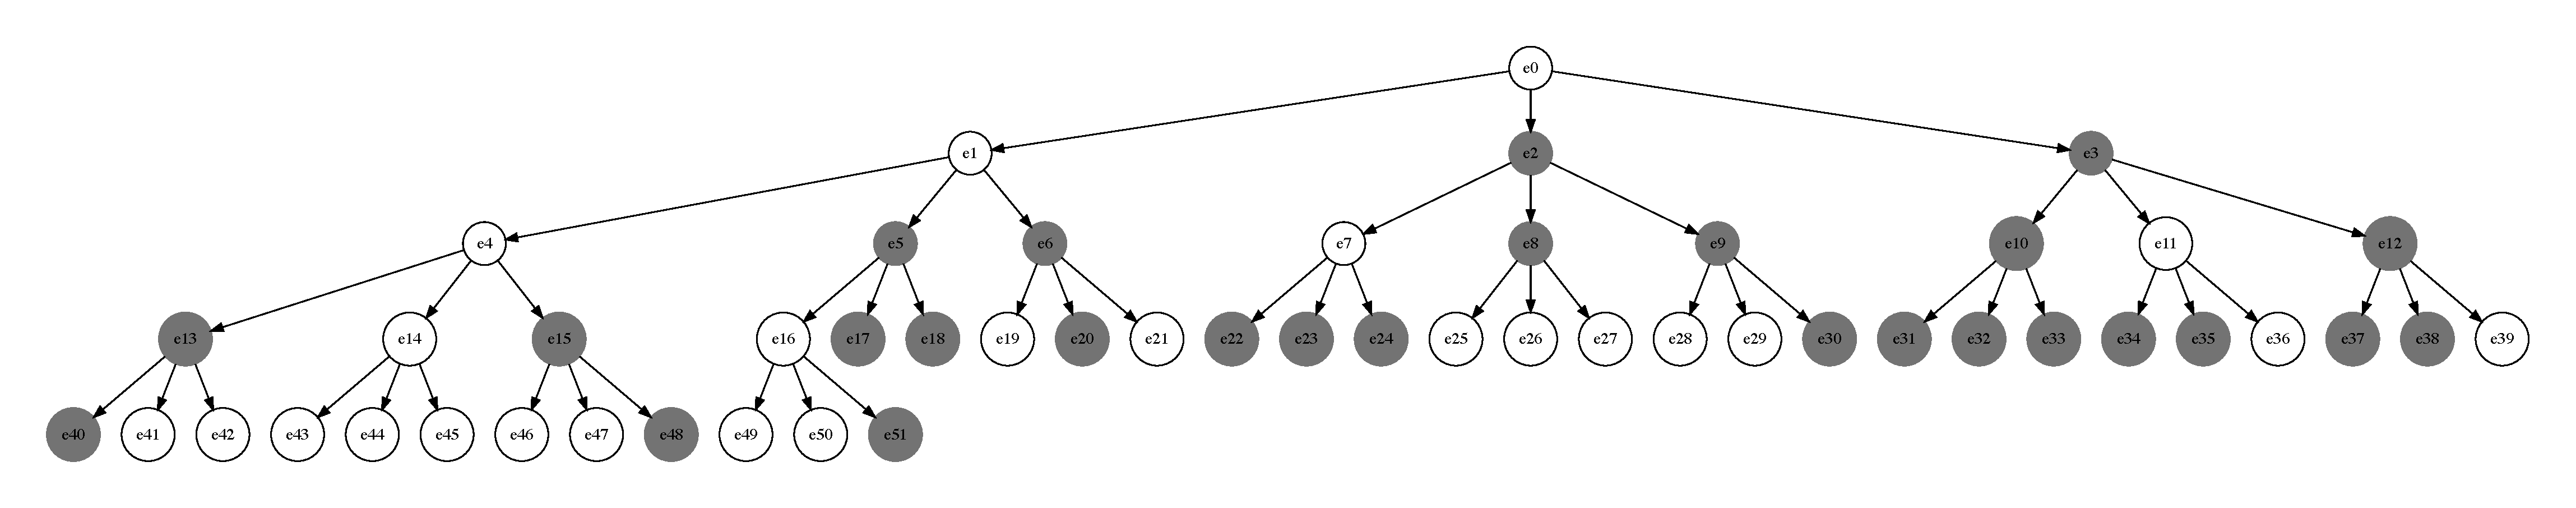
\includegraphics[width=\textwidth]{figs/Uni-hierachy.pdf}
  \end{minipage}
\end{figure}

For each employee, we use the generative model of Figure~\ref{fig:BN} to draw assignments for all the random variables. We assume that only $40\%$ of employees are qualified for promotion and regardless of their labels, employees submit only $60\%$ of their opinions. In addition, due to various personal and environmental factors, only $60\%$ of high quality employees perform well while $10\%$ of low quality employees also perform well regardless of their labels. Note that these numbers are not specific and just chosen for the framework to serve as a representative setting and a proof of concept. The conditional probability table for the opinion variable $O$ is parameterized by four values $(\theta_1, \theta_2, \theta_3, \theta_4)$ which together determine the degree of discrimination against the protected group. Since other parameters in the Bayesian network did not have a direct effect on the degree of discrimination, we fixed them to arbitrary values. 

The results presented in this section are based on an organization hierarchy  with $100$ employees where $k=5$. However, the results of the framework are not sensitive to the settings as we test the framework with various organization sizes ranging from $50$ to $500$ employees and various degree for $k$ ranging from $3$ to $10$. We generated seven datasets given the organization hierarchy using different values for the $\theta$ parameters: $(0.0,1.0,0.0,0.0)$, $(0.33,1.0,0.0,0.0)$, $(0.66,1.0,0.0,0.0)$, $(1.0,1.0,0.0,0.0)$, $(1.0,1.0,0.0,0.33)$, $(1.0,1.0,0.0,0.66)$, $(1.0,1.0,0.0,1.0)$. 
 
In the first three settings the discrimination originates from negative opinions towards qualified outgroup employees. The first setup is an extreme case where the opinion towards outgroup employees is always negative. The discrimination in the last three settings originates from positive opinions towards unqualified ingroup employees. The last setup is an extreme case where the opinion towards ingroup employees is always positive. The fourth setup represent unbiased opinions where employees are treated similarly based on their qualification. 

\paragraph{MAP Inference} We use the model presented in Table~\ref{tab:pslmodel} for MAP inference in PSL and FairPSL (recall that in FairPSL, the $\delta$-fairness constraints corresponding to one of the fairness measures are also added to the model). The observed atoms are $\textit{Manager(m,e)}$, $\textit{PositiveReview(e1,e2)}$ and labels of all employees. The truth values for all other atoms are obtained via MAP inference. We use the truth values obtained for the decision atoms $\textit{ToPromote(e)}$ to compute the fairness measures. We defined the discriminative pattern, and the protected and unprotected groups of this problem in Section~\ref{sec:formulation}.


\subsection{Evaluation results}

\begin{figure}
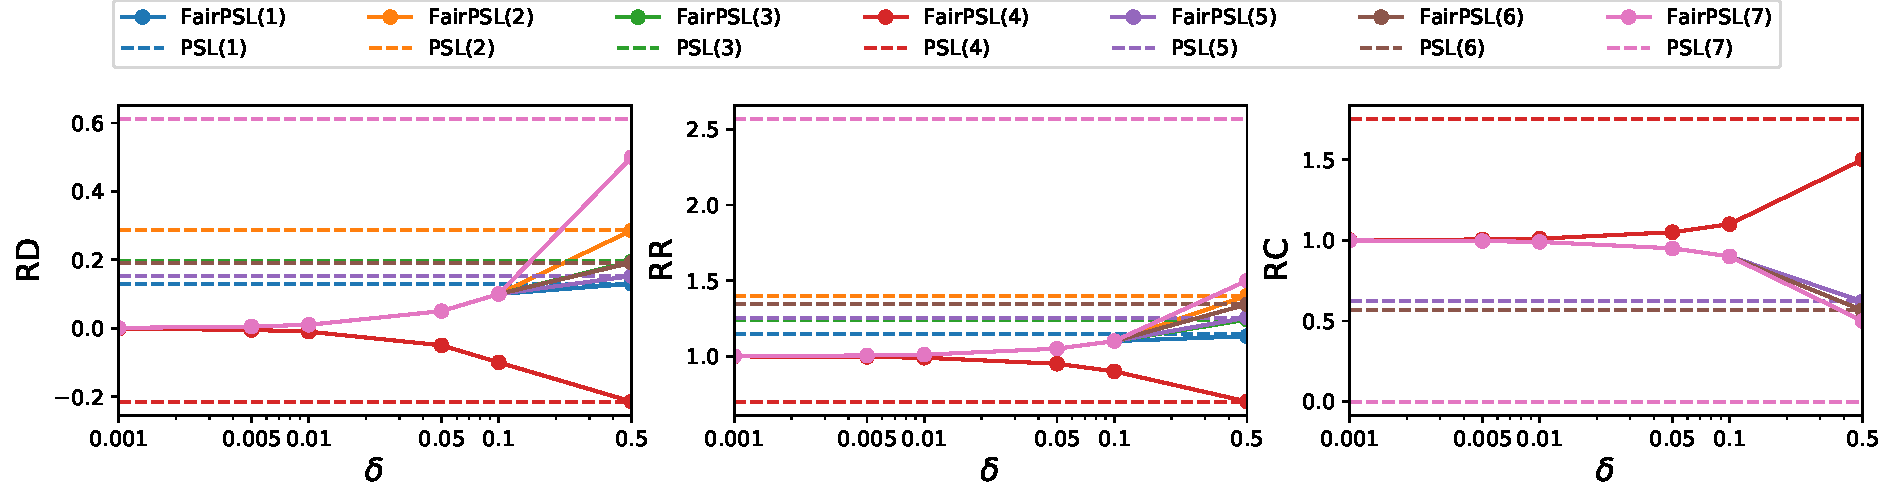
\includegraphics[width=1\linewidth]{figs/results_vis_uni_params.pdf}
\caption{\small Fairness score of predictions obtained by MAP inference of PSL and FairPSL, according to the fairness measures \emph{RD}, \emph{RR}, and \emph{RC}. The labels of datasets are mentioned with parenthesis next to the inference method. The FairPSL values of each measure are obtained by adding the $\delta$-fairness constraint of that measure.\label{fig:results}
}  
\end{figure}

To answer \textbf{Q1}, we run the MAP inference algorithm of PSL and FairPSL on seven synthetic datasets. 
We run the MAP inference of FairPSL multiple times on each dataset: For each of the three fairness measures, we add the corresponding $\delta$-fairness constraint with five thresholds $\{0.001, 0.005, 0.01, 0.05, 0.1, 0.5\}$.

Figure~\ref{fig:results} shows the fairness score of predictions in terms of the three fairness measures. As expected, tighter $\delta$-fairness constraints lead to better scores. Note that the best possible score according to RD is 0, as it computes a difference. Since RR and RC compute ratios, the best possible score according to these measures is 1. In our experiments, with any of these measures, taking $\delta = 0.001$ pushes the score of predictions to its limit.  

The $\delta$-fairness constraints modify the optimization problem of MAP inference by reducing the feasible region to solutions that conform with fairness guarantees. Research question \textbf{Q2} is concerned with the effect of this reduction on the accuracy of predictions. Note that decision quality is the same as the accuracy of predictions. To answer this question, we compare the inferred values for the decision atoms \textit{ToPromote(e)} against their actual values. These values are extracted from the known values of \textit{IsQualified(e)} according to rules 11 and 12 in Table~\ref{tab:pslmodel}. Figure~\ref{fig:accuracy} shows the area under the curve of the receiver operating characteristic~(AUC) of predicting the decision variable in three groups, namely the protected group, the unprotected group (i.e., promotion of the employees who have in-group managers), and all employees. By doing so, we make sure that our fairness constraints do not propagate bias towards either of the populations. Since the results of FairPSL with $\delta$-fairness constraints RR and RC are very similar to the results of RD, we only report the latter here.


\begin{figure}
    \centering
    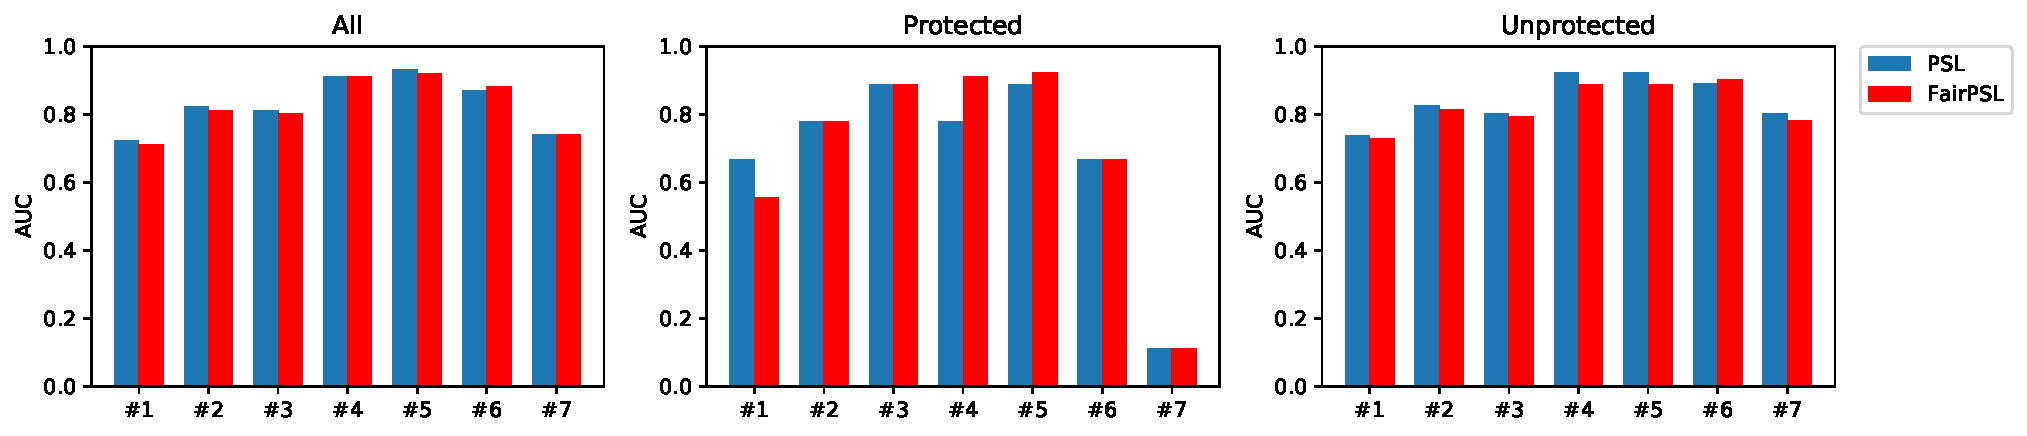
\includegraphics[width=\textwidth]{figs/roc.pdf}
    \caption{\small AUC score of predictions for truth values of unknown atoms \textit{ToPromote(e)} using MAP inference of PSL and FairPSL with $\delta$-fairness constraints $RD$ with $\delta=0.001$.}
    \label{fig:accuracy}
\end{figure}

According to Figure~\ref{fig:accuracy}, the results of both PSL and FairPSL in all seven datasets are close to each other. Note that although fairness may impose a cost in terms of overall accuracy, FairPSL often improves the accuracy of the protected class. Sometimes the overall predictions of FairPSL are even slightly better than PSL (e.g., dataset 6 and 7). As expected, the accuracy of the fourth setting where the opinions are unbiased are similar in both PSL and FairPSL. We observe that prediction of MAP inference for both FairPSL and PSL are similar, thus, in these settings at least, FairPSL guarantees fairness without hurting accuracy. Further investigation is required on the effect of the various ranges of discrimination (i.e., $\theta_1$, $\theta_2$, $\theta_3$, $\theta_4$) on the prediction results of FairPSL.



We also generate various types of organizations in which labels are not uniformly distributed, e.g., one population only occurs at the bottom levels of an organization. While we did not observe any differences in the behavior of our method with respect to accuracy and fairness measure, we found that the degree of discrimination is higher in such organizations. Further investigations on the structure of an organization on discrimination is an interesting direction for future research. 

\section{Conclusion and Future Directions}
\label{sec:conclusion}
Many applications of AI and machine learning affect peoples' lives in important ways. While there is a growing body of work on fairness in AI and ML, it assumes an individualistic notion of fairness.   In this paper, we have proposed a general framework for relational fairness which includes both a rich language for defining discrimination patterns and an efficient algorithm for performing inference subject to fairness constraints. We show our approach enforces fairness guarantees while preserving the accuracy of the predictions. 

There are many avenues for expanding on this work. For example, here we assumed that the discriminative pattern is given, however an automatic mechanism to extract discriminatory situations hidden in a large amount of decision records is an important and required task. Discrimination discovery has been studied for attribute-based fairness~\cite{pedreschi2013discovery}. An interesting next step is discrimination pattern discovery in relational data.

\section*{Acknowledgements}
This work is supported by the National Science Foundation under Grant Numbers CCF-1740850 and IIS-1703331. Golnoosh Farnadi and Behrouz Babaki are  supported by postdoctoral scholarships from IVADO through the Canada First Research Excellence Fund (CFREF) grant.

\begin{thebibliography}{10}
\itemsep=1pt 
\begin{small}

\bibitem{EUlaw}
European union legislation. (a) racial equality directive, 2000; (b) employment
  equality directive, 2000; (c) gender employment directive, 2006; (d) equal
  treatment directive (proposal), 2008.

\bibitem{UKlaw}
{UK} legislation. (a) sex discrimination act, 1975, (b) race relation act,
  1976.

\bibitem{USlaw}
United nations legislation. (a) universal declaration of human rights, 1948,
  (c) convention on the elimination of all forms of racial discrimination,
  1966, (d) convention on the elimination of all forms of discrimination
  against women, 1979.

\bibitem{alshukaili:iswc16}
Duhai Alshukaili, Alvaro A.~A. Fernandes, and Norman~W. Paton.
\newblock Structuring linked data search results using probabilistic soft
  logic.
\newblock In {\em International Semantic Web Conference {(1)}}, volume 9981 of
  {\em Lecture Notes in Computer Science}, pages 3--19, 2016.

\bibitem{bach:jmlr17}
Stephen~H. Bach, Matthias Broecheler, Bert Huang, and Lise Getoor.
\newblock Hinge-loss markov random fields and probabilistic soft logic.
\newblock {\em Journal of Machine Learning Research}, 18:109:1--109:67, 2017.

\bibitem{barocas2016big2}
Solon Barocas and Andrew~D Selbst.
\newblock Big data's disparate impact.
\newblock {\em California Law Review}, 104:671, 2016.

\bibitem{boyd2014networked}
Danah Boyd, Karen Levy, and Alice Marwick.
\newblock The networked nature of algorithmic discrimination.
\newblock In {\em Data and discrimination: Collected essays}, pages 53--57.
  2014.

\bibitem{brewer1979group}
Marilynn~B Brewer.
\newblock In-group bias in the minimal intergroup situation: A
  cognitive-motivational analysis.
\newblock {\em Psychological bulletin}, 86(2):307, 1979.

\bibitem{brewer2007social}
Marilynn~B Brewer.
\newblock The social psychology of intergroup relations: Social categorization,
  ingroup bias, and outgroup prejudice.
\newblock {\em Social Psychology: Handbook of Basic Principles}, 2007.

\bibitem{chouldechova2017fair2}
Alexandra Chouldechova.
\newblock Fair prediction with disparate impact: {A} study of bias in
  recidivism prediction instruments.
\newblock {\em CoRR}, abs/1703.00056, 2017.

\bibitem{dwork2012fairness3}
Cynthia Dwork, Moritz Hardt, Toniann Pitassi, Omer Reingold, and Richard~S.
  Zemel.
\newblock Fairness through awareness.
\newblock In {\em {ITCS}}, pages 214--226. {ACM}, 2012.

\bibitem{ebrahimi:emnlp16}
Javid Ebrahimi, Dejing Dou, and Daniel Lowd.
\newblock Weakly supervised tweet stance classification by relational
  bootstrapping.
\newblock In {\em {EMNLP}}, pages 1012--1017. The Association for Computational
  Linguistics, 2016.

\bibitem{farnadi2018fairness}
Golnoosh Farnadi, Behrouz Babaki, and Lise Getoor.
\newblock Fairness in relational domains.
\newblock In {\em AAAI/ACM Conference on AI, Ethics, and Society (AIES)}, pages
  108--114. ACM, 2018.

\bibitem{feldman2015certifying2}
Michael Feldman, Sorelle~A. Friedler, John Moeller, Carlos Scheidegger, and
  Suresh Venkatasubramanian.
\newblock Certifying and removing disparate impact.
\newblock In {\em {KDD}}, pages 259--268. {ACM}, 2015.

\bibitem{getoor2007introduction}
Lise Getoor and Ben Taskar.
\newblock {\em {Introduction to Statistical Relational Learning}}.
\newblock MIT press Cambridge, 2007.

\bibitem{hardt2016equality3}
Moritz Hardt, Eric Price, and Nati Srebro.
\newblock Equality of opportunity in supervised learning.
\newblock In {\em {NIPS}}, pages 3315--3323, 2016.

\bibitem{kamishima2011fairness}
Toshihiro Kamishima, Shotaro Akaho, and Jun Sakuma.
\newblock Fairness-aware learning through regularization approach.
\newblock In {\em ICDMW}, pages 643--650. {IEEE} Computer Society, 2011.

\bibitem{kouki:recsys15}
Pigi Kouki, Shobeir Fakhraei, James~R. Foulds, Magdalini Eirinaki, and Lise
  Getoor.
\newblock Hyper: {A} flexible and extensible probabilistic framework for hybrid
  recommender systems.
\newblock In {\em RecSys}, pages 99--106. {ACM}, 2015.

\bibitem{counterfactualfairness}
Matt~J. Kusner, Joshua~R. Loftus, Chris Russell, and Ricardo Silva.
\newblock Counterfactual fairness.
\newblock In {\em {NIPS}}, pages 4069--4079, 2017.

\bibitem{Pedreschi:2012}
Dino Pedreschi, Salvatore Ruggieri, and Franco Turini.
\newblock A study of top-k measures for discrimination discovery.
\newblock In {\em {SAC}}, pages 126--131. {ACM}, 2012.

\bibitem{pedreschi2013discovery}
Dino Pedreschi, Salvatore Ruggieri, and Franco Turini.
\newblock The discovery of discrimination.
\newblock In {\em Discrimination and Privacy in the Information Society},
  volume~3 of {\em Studies in Applied Philosophy, Epistemology and Rational
  Ethics}, pages 91--108. Springer, 2013.

\bibitem{ridgeway2004unpacking}
Cecilia~L Ridgeway and Shelley~J Correll.
\newblock Unpacking the gender system: A theoretical perspective on gender
  beliefs and social relations.
\newblock {\em Gender \& society}, 18(4):510--531, 2004.

\bibitem{sridhar:bioinformatics16}
Dhanya Sridhar, Shobeir Fakhraei, and Lise Getoor.
\newblock A probabilistic approach for collective similarity-based drug-drug
  interaction prediction.
\newblock {\em Bioinformatics}, 32(20):3175--3182, 2016.

\bibitem{verma2018fairness2}
Sahil Verma and Julia Rubin.
\newblock Fairness definitions explained.
\newblock In {\em 2018 IEEE/ACM International Workshop on Software Fairness
  (FairWare)}, pages 1--7. IEEE, 2018.

\bibitem{west2014exploiting}
Robert West, Hristo~S. Paskov, Jure Leskovec, and Christopher Potts.
\newblock Exploiting social network structure for person-to-person sentiment
  analysis.
\newblock {\em {TACL}}, 2:297--310, 2014.

\bibitem{zafar2017parity}
Muhammad~Bilal Zafar, Isabel Valera, Manuel Gomez{-}Rodriguez, Krishna~P.
  Gummadi, and Adrian Weller.
\newblock From parity to preference-based notions of fairness in
  classification.
\newblock In {\em {NIPS}}, pages 228--238, 2017.

\bibitem{zemel2013learning}
Richard~S. Zemel, Yu~Wu, Kevin Swersky, Toniann Pitassi, and Cynthia Dwork.
\newblock Learning fair representations.
\newblock In {\em {ICML} {(3)}}, volume~28 of {\em {JMLR} Workshop and
  Conference Proceedings}, pages 325--333. JMLR.org, 2013.

\end{small}
\end{thebibliography}

\end{document}

\end{article}


\begin{article}
{Accelerating the Machine Learning Lifecycle with {MLflow}}
{Matei Zaharia, Andrew Chen, Aaron Davidson, Ali Ghodsi, Sue Ann Hong, Andy Konwinski, Siddharth Murching, Tomas Nykodym, Paul Ogilvie, Mani Parkhe, Fen Xie, Corey Zumar}
\graphicspath{{submissions/mlflow/}}
\documentclass[11pt]{article}

%\usepackage{deauthor}

%\usepackage{times}

%\usepackage[pdftex]{graphicx}
%\DeclareGraphicsExtensions{.pdf,.jpeg,.jpg,.png}
%\graphicspath{{soumagne/}}

%\usepackage[affil-it]{authblk}
%\setlength{\affilsep}{0em}

%\usepackage[labelfont=bf,labelsep=space,list=true]{subcaption}

%\usepackage{url}

\begin{document}
\title{Advancing RPC for Data Services at Exascale}
\author[1]{Jerome Soumagne}
\author[2]{Philip Carns}
\author[2]{Robert B. Ross}
\affil[1]{The HDF Group}
\affil[2]{Argonne National Laboratory}

\maketitle

\begin{abstract}
Remote Procedure Call (RPC) has long been an inherent component of parallel
file systems and I/O forwarding middleware in high-performance computing
(HPC).  RPCs are used in this environment to issue
I/O operations and transfer data from compute nodes to gateway and server storage
nodes. With HPC systems becoming more heterogeneous, data volumes
reaching new thresholds, and I/O standing as the main bottleneck, there is a growing
need in the HPC community to build distributed services and adopt new workflows
that are, nonetheless, no longer dictated by monolithic parallel file systems. These include
specialized storage, data analysis, and telemetry
services that can be adapted to fit application needs. Parallel file system
RPC facilities have never been exposed to service or middleware developers,
however, leaving them with two choices: MPI or the low-level fabric network
protocol.
In this article, we show how an independent RPC framework can be used as a building block for
developing user-level data services at exascale. We identify the design
choices that must be considered in terms of both performance and resilience
for HPC
data services, and we discuss the directions taken to palliate current HPC system constraints.
\end{abstract}

\section{Introduction}
\label{sec:intro}

High-performance computing (HPC) facilities have traditionally
been designed around \textit{monolithic} file systems, which are tailored to
scientific HPC workflows comprised of computation, storage, and
data analysis. Scientific application users, whose needs depend
on the application's domain, have been constrained to conform to system precepts
and this standard workflow. While this has been
a viable (but increasingly limiting) option for pre-exascale systems,
increasing data volumes and increasing system complexity with
emerging hardware are now forcing application users to adopt new
\textit{specialized} workflows.  These specialized workflows not only achieve sustainable
performance and perform data analysis in a timely manner at an increasing
scale, but also better respond to application needs and provide data
insights, for example through monitoring and telemetry service.

Creating specialized workflows requires the introduction of
a collection of \textit{data services} to the HPC ecosystem that must interact
with both the
system components (hardware and software) and the application.
While some of those services may be provided by the system, the vast majority
of data services are user-level services that are developed to augment the
original HPC system software stack and better serve the application's
performance or functionality needs. Data services (system-provided
or user-provided) must respond, in most cases, to the same user
prerequisites by ensuring performance, resilience, and ease of deployment.
These prerequisites introduce engineering challenges that
must be overcome when creating a new HPC data service---by no means an
easy task. One such challenge is communication: data exchange
between services is a critical aspect of
specialized workflows that are composed of multiple services interacting with
each other. Developing the messaging part of a data service component on an HPC
machine can, for a new service developer, involve either using the
low-level network fabric
API, which requires a significant amount of work and expertise, or using the vendor installed
MPI library~\cite{mpich} that takes advantage of the underlying network fabric. 
MPI itself, however, is not very suitable for developing such dynamical services that
may come and go
%, nor is it suitable for efficiently accessing memory of a remote process
%without prior collective synchronization
~\cite{Zounmevo2013}.
%
MPI implementations have consistently prioritized use
by applications and not by service libraries.

Data services are already a well-established technology in the cloud, where
remote procedure call (RPC) is the main technique used for sending messages
to remote components. Google gRPC~\cite{protobuf} or Facebook Thrift~\cite{Slee2007}
are good examples of such
frameworks. However, they are not well-suited to run on HPC systems because they (1)
rely on the TCP/IP stack and do not take advantage of the low latency/high
bandwidth HPC fabrics and (2) are not designed for exchanging very large amounts
of data, a task that is left to the user.
In contrast, RPC has been used as the communication pillar of
distributed file systems (e.g., Lustre Networking (LNET)~\cite{Wang2009},
Panasas~\cite{Welch2008}) and I/O forwarding layers
(e.g., IOFSL~\cite{Ali2009}) that are specifically designed to send I/O requests on top of the
underlying network fabric. The Network File System (NFS)~\cite{Sandberg1988}
is also a good example of the use of RPC with large data transfers and
therefore close to the use of RPC in an HPC system.
The internal RPC facilities of these file systems (with the exception of NFS) have,
nonetheless, never
been directly exposed to users; instead, they have been deeply buried in the
monolithic file system software stacks that often extend into kernel space.
Other parallel file systems have implemented their own network abstraction layer
to support multiple network fabrics
and provide messaging capabilities that can support data services. However, they are not
general-purpose RPC frameworks, and in most cases cannot be easily extracted
from the file systems that they were designed for.

Based on both of those technologies and past experience with I/O forwarding,
we introduced in~\cite{Soumagne2013} an RPC framework, called Mercury, that takes
advantage of low-level HPC network fabrics and facilitates the development
of user-level data services. Mercury is part of a more comprehensive suite of components named
Mochi~\cite{Ross2020} that provides
a collection of service components for the creation of specialized data services.
We present in this paper how some of the design
choices made for Mercury are essential for building an heterogeneous service
workflow in an exascale HPC environment. In Section~\ref{sec:related}, we
present some of the work that
is similar to Mercury and approaches that we take to develop user-level data
services. In Section~\ref{sec:overview}, we give a brief overview of Mercury's
architecture before focusing in Section~\ref{sec:design} on the specific design
points that make an RPC framework usable for HPC data services, supporting our
claims by evaluation results. In Section~\ref{sec:apps}, we present some of the data services that are
successfully being deployed using Mochi and Mercury.
In Section~\ref{sec:concl}, we summarize our conclusions.

\section{Related Work}
\label{sec:related}

A few other frameworks and suites of HPC data service components have been proposed
using an approach similar to the one we used in Mercury. We present here
three of the most notable frameworks.

\textit{DataSpaces}~\cite{Docan2012} implements a
scalable, semantically specialized shared-space abstraction that is
dynamically accessible by all components and services in an application
workflow, supporting both application/system-aware data placement and data movement.
It relies on the \textit{Decoupled and Asynchronous Remote Transfers} (DART)~\cite{Docan2010}
layer, which is not defined as an explicit RPC framework, although it allows transfer of
large amounts of data using a client/server model from applications running on
the compute nodes of an HPC system to local storage or remote locations, in
order to enable remote application monitoring, data analysis, code coupling,
and data archiving.
The key requirements that DART seeks to satisfy are minimizing data transfer
overheads on the application; achieving high throughput, low latency data
transfers; and preventing data losses. To this end, DART is
designed so that dedicated nodes (i.e., separate from the application compute
nodes) asynchronously extract data from the memory of the compute nodes using
remote direct memory access (RDMA).

The \textit{Scalable Observation System} (SOSflow)~\cite{Wood2016} provides a broad
set of online and in situ capabilities, including code steering via remote method
invocation, data analysis, and visualization. SOSflow can couple together
multiple sources of data, such as application components and operating
environment measures, with multiple software libraries and performance
tools. SOSflow's communication mechanism relies both on TCP sockets for
on-node communication and on MPI for off-node communication. Its main communication
pattern is a publish-and-subscribe mechanism and relies on a daemon that is
launched as a background  process  in  user space at the start of a
job script, before the scientific workflow begins.

\textit{Faodel}~\cite{Ulmer2018} provides a set of services for data
management and exchange in HPC workflows. Three major components of
Faodel are Kelpie, Opbox, and Lunasa. Kelpie provides a key-blob
abstraction. OpBox is a library for implementing asynchronous communication
between multiple entities in a distributed application, and provides the user
with primitives for expressing a protocol as a state machine that the
communication layer can process in an asynchronous manner. It also provides
a naming service to locate components of an application. Lunasa provides
user-level network memory management services and effectively
acts as a memory registration cache for doing RDMA. Faodel relies on
an evolution of the NNTI layer from the \textit{NEtwork Scalable
Service Interface} (Nessie)~\cite{Lofstead2011} RPC library.
It provides an asynchronous RPC solution, designed to overlap computation and
I/O. Nessie also provides a mechanism to handle bulk data transfers, which can use
RDMA to transfer data efficiently from one memory to the other, and supports
several network transports. Nessie uses the RPC interface to push
control messages to the servers and exposes a separate one-sided API that is
used to push or pull data between client and server.

\section{Overview and Considerations}
\label{sec:overview}

Mercury is designed around three key paradigms: provide reliable RPC
functionality, support large data arguments, and take advantage of the HPC network
fabrics. In terms of functionality, much more is needed when
developing distributed HPC data services; but as opposed to RPC frameworks that are
part of monolithic software stacks, Mercury remains as thin as possible
in order to allow for reusability between various service components that must
support different needs.

\begin{figure}[h]
\centering
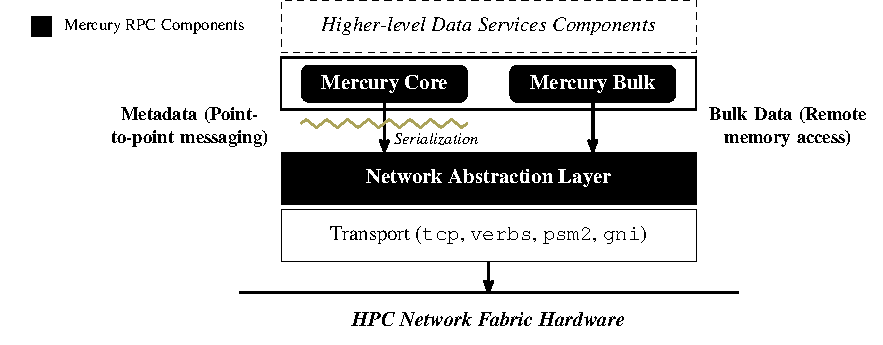
\includegraphics{figs/overview}
%\vspace{-5pt}
\caption{Overview of Mercury RPC components in the software stack.}
\label{fig:overview}
%\vspace{-10pt}
\end{figure}

As shown in Figure~\ref{fig:overview}, Mercury is composed of
two service-level components:
a core RPC component, which is designed to serialize
function arguments and send them to a remote target for execution using
point-to-point messaging, and a bulk
component, which is designed to handle large arguments (i.e., arguments that are
generally larger than 4KB depending on the underlying protocol being used).
This latter component enables the creation of
memory descriptors that can be sent along with the other arguments to the RPC
target to initiate raw memory transfers (without serialization) using remote memory access (RMA).
In Section~\ref{sec:rdma}, we detail this scenario and its benefits.
%
In order to support a large variety of HPC network fabrics,
both of these components interface with a network abstraction
layer that provides a minimum set of network primitives for both
point-to-point messaging and one-sided RMA communication operations.
Moreover, in order to reduce the burden of connection handshakes
when the underlying network does not necessarily request it (also
essential for scalability) and to support services that may come and go,
remote peers are addressed through unconnected endpoints.
Furthermore, in order to maximize throughput, all communication is made
nonblocking through a callback-based approach that we detail in
Section~\ref{sec:cb}.

While these points describe the overall architecture of an RPC
framework for HPC, additional key items can rapidly become prerequisites for
creating an RPC framework that is designed to support data services. These
include maximizing throughput, providing scaling, 
enabling flexibility, and ensuring resilience. In the
following section we describe how one can enhance RPC to (1) leverage RDMA-capable networks;
(2) support node-local service scaling and leverage multi-core processors;
(3) enable flexible, node-local deployment scenarios and service 
composition; (4) bridge nodes between multiple HPC networks; (5) enable fault tolerance.

\section{Enabling RPC for HPC Data Services}
\label{sec:design}

We do not compile an exhaustive list of features in this section.
%
Instead, we focus on those features that are necessary to enable strong service scaling,
performance, flexibility, and resilience for data services on emerging
large-scale computing platforms.

\subsection{HPC Network Support}
\label{sec:rdma}

As opposed to cloud-based RPC solutions that rely on TCP networking,
HPC network fabrics provide dedicated solutions that offer both
low latency and high bandwidth. To take advantage of these solutions, however, 
an RPC framework must leverage low-level vendor APIs such as InfiniBand{\small \texttrademark} Verbs,
Intel{\textsuperscript{\textregistered}} Performance Scaled Messaging 2 (PSM2),
and Cray{\textsuperscript{\textregistered}} Generic Network Interface (GNI).
Rather than implementing Mercury's network
abstraction layer directly on top of those APIs, we currently use
OFI libfabric~\cite{Grun2015} as
the intermediate layer that abstracts RDMA capabilities for RDMA-capable
networks or emulated RMA (over point-to-point) for noncapable networks.
Exposing native RDMA primitives is essential for taking full advantage of RDMA
capable networks so that a data service can, for large data, leverage zero-copy
transfers from the application's memory from/to the storage.

\begin{figure}[h]
\centering
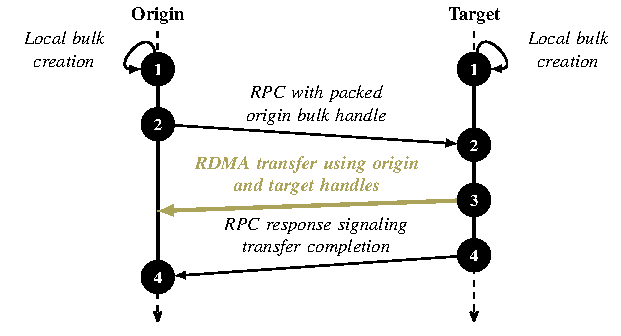
\includegraphics{figs/bulk_rdma}
\vspace{-5pt}
\caption{Four-step process of Mercury's bulk RDMA transfers.}
\label{fig:bulk_rdma}
\vspace{-10pt}
\end{figure}

Enabling RMA capabilities through Mercury's bulk component (see Figure~\ref{fig:overview})
is a four-step process (see Figure~\ref{fig:bulk_rdma}).
First, \textit{bulk handles}, which are abstract memory
descriptors, must be created on both origin and target processes. During
handle creation, memory regions are registered (which in most cases
corresponds to a physical hardware registration); this allows for the
higher level data service to only expose memory pages that it wishes to access in either
read-write or read-only mode. Second, an RPC is issued from the origin
process to the target process with the serialized bulk handle of the origin process;
this handshake allows the target process to gather virtual address information,
registration keys, and so forth, which are necessary for the underlying protocol to post
an RDMA operation.
Third, the actual RDMA operation is posted using both the target's local bulk handle
and the origin's handle that was transmitted through the RPC. Since bulk handles are
abstract memory descriptors, more complex scenarios such as scatter/gather can
be transparently implemented and even delegated to the hardware if the hardware provides this support,
allowing for more efficient transfers. Finally, the RPC response is sent, effectively 
signaling the origin of the transfer completion. This server-driven four-step process is
the most conventional model for data transfers in Mercury, but client-driven transfers are legal
as well. The former is
more commonly recommended for two reasons. First, it enables servers to throttle or
re-order
transfers according to load.  Second, it makes the clients lighter weight and more scalable,
since they do not have to track the state of server resources.

\paragraph{Evaluation.}
To show the importance of supporting this capability, we compare the RPC performance and ``RPC with bulk'' performance
on an InfiniBand cluster (Cooley) that is equipped with 4X FDR Infiniband cards (56 Gb/s).
Compared to TCP over the same network,
our approach improves RPC throughput with close to
$9\times10^{5}$ operations per second and close to 6,000 MB/s average throughput when performing RPC and bulk transfer through the native verbs interface.
Note that the previous results do not use any multi-threading capabilities. We maintain
a number of 32 RPCs in-flight to ensure sustained performance. Multi-threading support is
discussed in the next section.

\begin{figure*}[h]
\subfloat[RPC round-trip benchmark (32 RPCs in-flight).\label{fig:rpc_rate_verbs}]{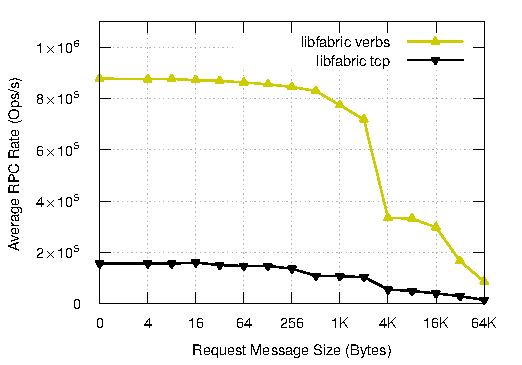
\includegraphics[width=0.49\linewidth]{figs/rpc_rate_verbs} }
\subfloat[Bulk transfer (server pull) benchmark (32 RPC in-flight).\label{fig:write_bw_verbs}]{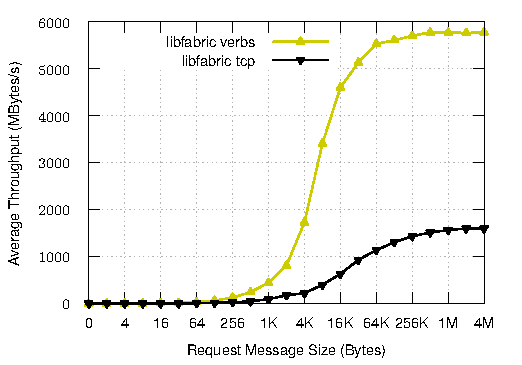
\includegraphics[width=0.49\linewidth]{figs/write_bw_verbs} }
\caption{Effect of leveraging RDMA network on InfiniBand cluster (FDR InfiniBand).}
\label{fig:bench_verbs}
\end{figure*}

\subsection{Multi-Core Architecture Support}
\label{sec:local_scaling}

With CPUs experiencing increasing core count and lower frequencies per
core, data services are expected to take advantage of these architectures
by either distributing the load of incoming RPCs across cores or by
running multiple services co-located within the same node.
% One of the points that we have not detailed so far is Mercury's progress model.
%
Communication
frameworks typically adopt one of two progress models: either \textit{explicit} or
\textit{implicit}. \textit{Explicit} progress implies that the user will regularly
make progress calls to effectively check into network completion queues, poll
file descriptors, etc. In contrast, an \textit{implicit} progress model will 
make progress in background without any need for the user to be involved.
However, this usually involves a background progress thread 
running to make progress while operations are being posted. While
this may seem convenient, this ``hidden'' thread can become detrimental when
running concurrently with other user's threads, leading to unexpected scheduling
issues.
%
Therefore, to prevent this type of issues and give data services sufficient
flexibility in how progress is ensured, we follow an explicit progress
model.
%
RPC is not only about messaging and communication, it is also about
execution of user-defined function calls. When making progress, therefore, it is
often desirable to decouple the RPC execution activities from the network progress activities,
which leads us to actually adopt a \textit{progress-and-trigger} model
that gives services more control over the placement of the progress and
execution threads.
%
In this approach, implicit progress can be accomplished
by the user by having a thread calling progress in background. 

In a typical scenario, an RPC listener service will start posting RPC receive
operations with memory bound to the thread posting the operations.
%
Distributing the execution of these incoming RPCs across multiple threads
(e.g., using a thread pool) can lead to several context switches
at a significant performance penalty. To prevent this scenario, take
advantage of multi-core architectures, and allow for node-local service scaling
without costly creation of separate endpoints per thread, we make
use of \textit{scalable endpoints} (SEP) when available.
%
Scalable endpoints are provided through libfabric~\cite{Grun2015} but
can be extended through our network abstraction layer.
Scalable endpoints allow for
sharing a single endpoint resources between threads by assigning separate
transmit and receive contexts (including completion queues) to each thread. When SEPs
are used, context switches between threads no longer exist---
a fundamental advantage for RPC multi-core architectures.


\begin{figure*}[h]
\subfloat[RPC round-trip benchmark (32 RPCs in-flight).\label{fig:rpc_sep_gni}]{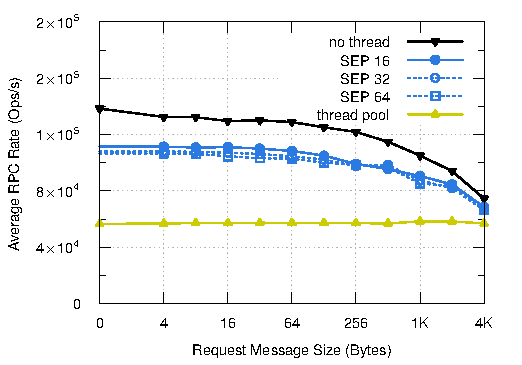
\includegraphics[width=0.49\linewidth]{figs/rpc_rate_sep_gni} }
\subfloat[Bulk transfer benchmark (32 RPC in-flight).\label{fig:write_bw_sep_gni}]{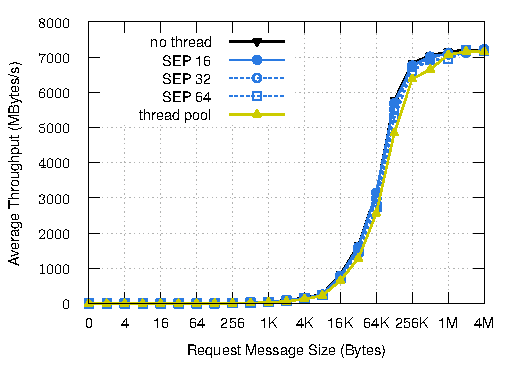
\includegraphics[width=0.49\linewidth]{figs/write_bw_sep_gni} }
\caption{Effect of using scalable endpoints on Cray XC40 (Aries interconnect).}
\label{fig:bench_sep_gni}
\end{figure*}

%\begin{figure*}[h]
%\begin{subfigure}[b]{.49\linewidth}
%\centering
%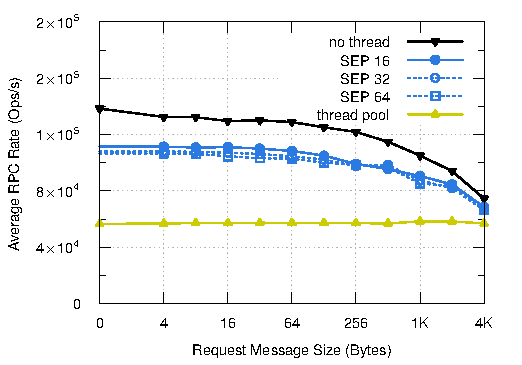
\includegraphics[width=\textwidth]{figs/rpc_rate_sep_gni}
%\caption{RPC round-trip benchmark (32 RPCs in-flight).}
%\label{fig:rpc_rate_sep_gni}
%\end{subfigure}%
%\hfill
%\begin{subfigure}[b]{.49\linewidth}
%\centering
%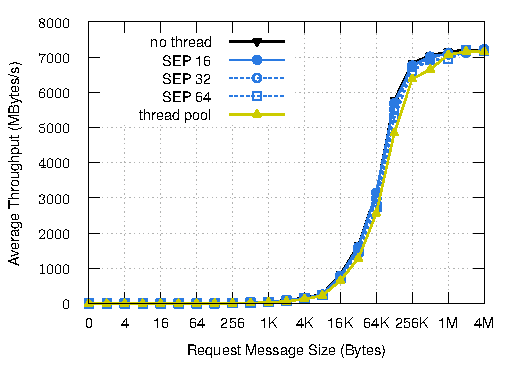
\includegraphics[width=\textwidth]{figs/write_bw_sep_gni}
%\caption{Bulk transfer benchmark (32 RPCs in-flight).}
%\label{fig:write_bw_sep_gni}
%\end{subfigure}
%\vspace{-5pt}
%\caption{Effect of using scalable endpoints on Cray XC40 (Aries interconnect).}
%\label{fig:bench_sep_gni}
%\vspace{-15pt}
%\end{figure*}

\paragraph{Evaluation.} To demonstrate the impact of context switches
and emphasize the benefits of scalable endpoints, we run two
benchmarks on the Theta supercomputer at the Argonne Leadership Computing Facility (ALCF).
Theta is a Cray XC40 system with a second-generation Intel Xeon Phi processor and
Cray Aries interconnect. Each compute node is a single Xeon Phi chip with 64 cores,
16 GB of Multi-Channel DRAM (MCDRAM), and 192 GB of DDR4 memory.
Users typically take advantage of this architecture by either deploying
multiple data services locally or by distributing incoming RPCs across cores.
%
In order to do so using SEP, we assign each core
to make progress and trigger calls on their own receive context.
As shown in Figure~\ref{fig:bench_sep_gni}, using SEP provides
close match (in terms of operations per second) to the performance of workloads
that do not use multi-threading. 
%
Distributing requests using a thread pool, in contrast, has a significant
detrimental impact on RPC rate.  Note that in all cases bulk transfers
exhibit similar overall bandwidth, as context switches only represent a
portion of the time spent when large data is transferred over the network.

\subsection{Flexible Provisioning and Topology}
\label{sec:local_deployment}

In the preceding section, we demonstrated node-level scaling when RPCs are made between
separate nodes using the native interconnect. Additional optimization can be made,
however, by being aware of node-local process placement, in order to ensure efficient
composition of services.

\subsubsection{Transparent Node-Local Deployment}

When deploying data
services, it is common for some of these services to either issue
RPCs to other local services (i.e., separate processes within the same node) or
to send RPCs back to themselves (i.e., within the same process).
The latter typically arises out of convenience, rather than creating a separate code path for
that case.
To achieve the former,
Mercury can make use of shared-memory transparently by detecting that
the target address is on the same node. Using lockless shared ring buffers and
lockless queues, it is possible to achieve lockless transfers with very low
latency. For bulk data transfers and to prevent any intermediate \textit{memcpy},
zero-copy transfers (i.e, one single and direct copy from origin to target buffer) can be
achieved using the Linux Cross-Memory Attach mechanism.

To achieve the latter, Mercury detects when the target address is the
same as the origin address and sends RPCs using the same argument packing mechanism,
by immediately queuing the RPC into a local completion queue, internally signaling
completion to wake up any potential thread waiting in a progress call. Likewise,
bulk data transfers are realized through a \textit{memcpy} between source and
destination buffers.

This combination of transparent shared-memory transfers between separate processes,
loopback redirection within the same process, and over-the-wire transfers has
shown substantial benefits when deploying data services in terms of performance
and flexibility, since data services can treat all three scenarios identically.


\begin{figure*}[h]
\subfloat[RPC round-trip benchmark (32 RPCs in-flight).\label{fig:rpc_rate_sm}]{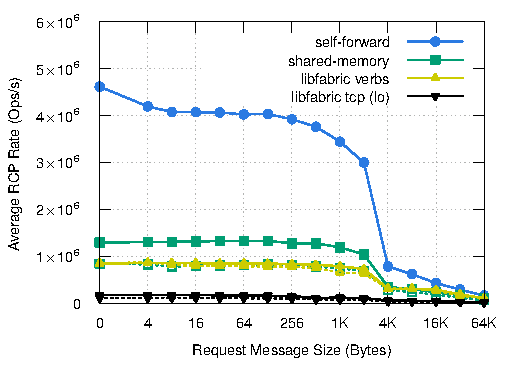
\includegraphics[width=0.49\linewidth]{figs/rpc_rate_sm} }
\subfloat[Bulk transfer benchmark (32 RPC in-flight).\label{fig:write_bw_sm}]{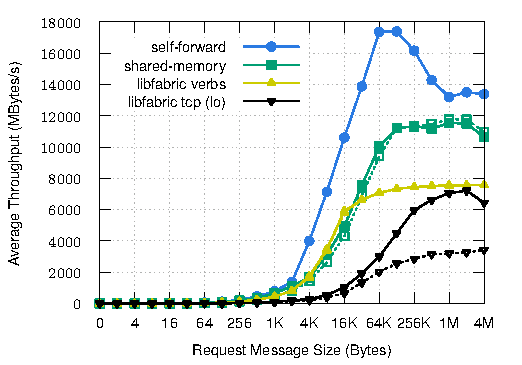
\includegraphics[width=0.49\linewidth]{figs/write_bw_sm} }
\caption{Comparison between node-local RPC mechanisms on InfiniBand cluster (FDR InfiniBand).}
\label{fig:bench_sm}
\end{figure*}

%\begin{figure*}[h]
%\begin{subfigure}[b]{.5\linewidth}
%\centering
%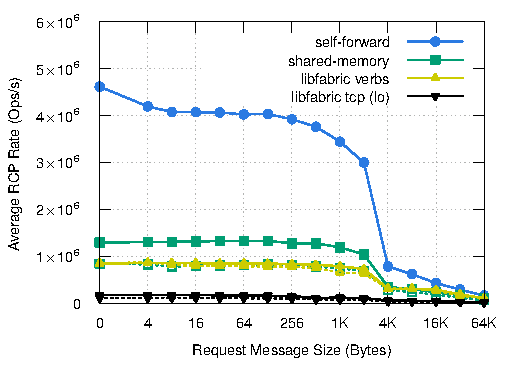
\includegraphics[width=\textwidth]{figs/rpc_rate_sm}
%\caption{RPC round-trip benchmark (32 RPCs in-flight).}
%\label{fig:rpc_rate_sm}
%\end{subfigure}%
%\hfill
%\begin{subfigure}[b]{.5\linewidth}
%\centering
%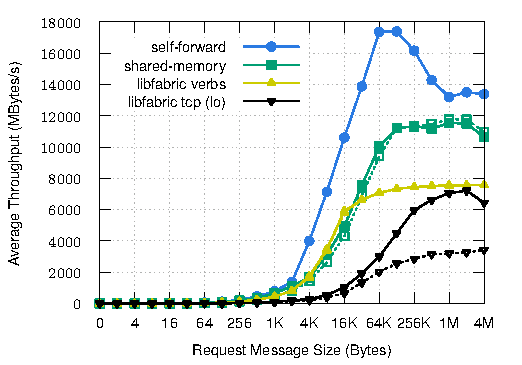
\includegraphics[width=\textwidth]{figs/write_bw_sm}
%\caption{Bulk transfer (server pull) benchmark (32 RPCs in-flight).}
%\label{fig:write_bw_sm}
%\end{subfigure}
%\vspace{-5pt}
%\caption{Comparison between node-local RPC mechanisms on InfiniBand cluster (FDR InfiniBand).}
%\label{fig:bench_sm}
%\vspace{-10pt}
%\end{figure*}

\paragraph{Evaluation.} To illustrate this scenario on our InfiniBand cluster (Cooley),
we compare in  Figure~\ref{fig:bench_sm} our two local RPC communication mechanisms 
to issuing RPCs either through the native interconnect (in this case InfiniBand Verbs)
or through TCP and the loopback interface. The latter is one of the fallback 
mechanisms typically used when not using shared-memory.
Cooley is equipped of dual-sockets nodes with Intel Xeon E5-2620 v3 CPUs. Consequently,
performance varies depending on process placement and the NUMA nodes being used---performance when running on separate NUMA nodes is represented by a dotted line in Figure~\ref{fig:bench_sm}.
In terms of both RPC
operations per second and bulk throughput, these two mechanisms are very valuable,
providing much better performance than both the native interconnect and TCP
(1.3 MOps/s for shared-memory and more than 4 MOps/s for loopback execution).
When running on separate NUMA nodes, shared-memory performance is naturally
impacted, though RPCs with bulk transfer still perform at a much higher rate due to the use
of Linux Cross-Memory Attach (CMA).

\subsubsection{Service Composition}

With node-level scaling and transparent node-local deployment in place,
composing data services seems the next natural step. In order to provide flexible composition, 
the RPC API must not be specific to any implementation but rather rely only on \textit{origin} and
\textit{target} concepts. The RPC mechanism then can be consistently employed to communicate
between different service ``servers'' and ``clients''.

\begin{figure}[h]
\centering
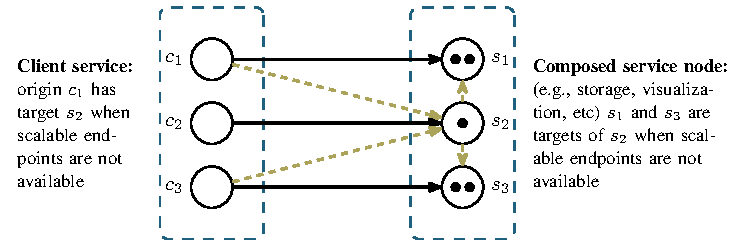
\includegraphics{figs/composition}
\caption{Composition of services with and without scalable endpoints.}
\label{fig:composition}
%\vspace{-5pt}
\end{figure}

When multiple services are colocated, there is also a need for addressing specific services and 
efficiently making progress. 
%
As shown in Figure~\ref{fig:composition}, this can then be accomplished by
using a ``delegator'' service, which can potentially become a bottleneck,
or by using scalable endpoints addressing specific receive contexts
directly through an ID that can be defined for each data service.
%
When there is no hardware support for scalable endpoints, however, this
functionality must be emulated by embedding a service ID into the RPC
header and using that ID to distribute RPC requests to the corresponding
service through that delegator.  An alternative is to create multiple
endpoints, one for each data service; but this is usually not recommended
due to hardware resource limitations.

\subsection{Multi-Network Support}

As we bridge local and nonlocal communication mechanisms, supporting multiple
fabrics follows a similar approach and relies on the same supporting
components described in Sections~\ref{sec:local_scaling} 
and~\ref{sec:local_deployment}. Mercury's architecture defines \textit{classes}
that physically correspond to one endpoint and \textit{contexts} that correspond
to completion queues and locally allocated resources. When using scalable endpoints
as described in Section~\ref{sec:local_scaling}, we are in a scenario with one class
(one endpoint) and multiple contexts (multiple completion queues) that share the same
endpoint. When bridging multiple fabrics, we are in a scenario with multiple classes 
(multiple endpoints) and one or more contexts (completion queues) associated with
each class.

The challenge is efficiently making progress over these separate
classes and contexts. To facilitate this, Mercury provides two progress
mechanisms, allowing for a service to either
%
busy spin on each of these contexts to process requests as quickly as possible (at the cost
of using more CPU resources), or to
%
wait and sleep on this set of contexts until a new request arrives.
%
In the latter case, we rely on Linux' file descriptor and \textit{epoll}
mechanism to wait. This allows for monitoring of both local event
notifications and hardware queue notifications. This transparent
notification mechanism allows a data service implementation to
simply wait on a file descriptor rather than manually making progress
on each of the interfaces/endpoints.

\subsection{Resilience and Fault Tolerance}
\label{sec:cb}

When supporting data services at scale, there are multiple approaches that one can take
to define a resilient RPC mechanism (for instance, guaranteed delivery).
One of the primary requirements for an RPC component is to allow services to
recover after a fault has occurred (e.g., node failure, unresponsiveness of a
service component) without compromising performance, by simply providing
robust support for canceling operations that are pending.
This implies reclaiming local resources that RPC operations have previously
allocated and gracefully recovering from faults.
It is important to note that we assume in that discussion the use of
\textit{reliable} unconnected endpoints in the transport layer, hence RPC requests
do not get ``lost''. Ordering and tag matching are not
critical for the transport to provide though (Mercury matches messages itself when needed).
Mercury itself only provides \textit{at-most} once semantics: nonblocking RPC
requests are sent and a nonblocking response is sent back (unless it is explicitly stated 
not to do so). It is then up to services to make their
own decision on how to react (e.g., retry, fail over, initiate a rebuild, etc).
Both RPC and bulk data transfer operations may be interrupted if any of the
peers involved no longer responds, in which case pending operations must be
canceled. Canceling an operation that cannot
complete, either because a fault has occurred or a timeout has been reached, 
is necessary in order to reach proper completion.

\begin{figure}[h]
\centering
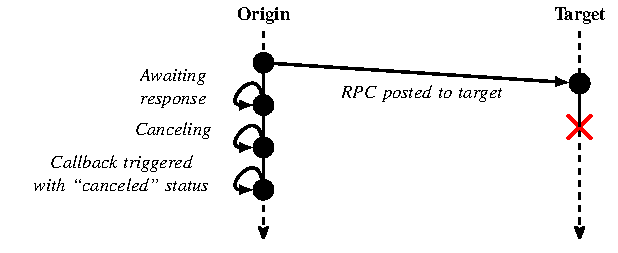
\includegraphics{figs/cancel}
%\vspace{-5pt}
\caption{Cancelation of an RPC operation.}
\label{fig:cancel}
%\vspace{-5pt}
\end{figure}

Cancelation of operations in Mercury is always an \textit{asynchronous} and
\textit{local} operation. As shown in Figure~\ref{fig:cancel}, forwarding an RPC
request is a nonblocking operation. Therefore, since Mercury follows a callback-based
mechanism, completion of that operation is known from a user's
perspective only when the callback that is associated to that operation
is pushed to the local completion queue and later triggered after making both
progress and trigger calls. When that callback is triggered, the state of the
operation is reported to the user as \textit{canceled}. Since operations are nonblocking,
keeping cancelation an asynchronous operation instead of an operation that completes
immediately is essential.
This mechanism protects against races in the event that a peer response arrives
after local cancelation has already succeeded. After the callback is triggered,
it is then safe to re-use the existing RPC request handle to issue a retry for example.

Cancelation is the foundation for implementing timeout scenarios in data services
in order to recover from a fault. When an internal
fault occurs, however, cancelation of the operation is not always necessary if the RPC
has not yet been posted, in which case that operation can simply be directly retried. This
scenario is similar for all other nonblocking operations in Mercury, including
bulk data transfers.

\section{Applications and Use Cases}
\label{sec:apps}

As mentioned in Section~\ref{sec:intro}, Mercury is part of the Mochi suite of service of components.
Mochi provides additional features on top of Mercury such as the notion of group membership,
transparent user-level thread semantics, key/value stores, C++ and Python bindings.
This work is further described in~\cite{Ross2020} along with
additional use cases, including the following:

Intel's \textit{Distributed Application Object Storage} (DAOS)~\cite{Intel2019} project
provides a transactional and multidimensional object store for
use in large-scale HPC environments with embedded storage directly
attached to the compute fabric. DAOS is a vendor-backed push to
provide an alternative to the traditional parallel file system and has the
potential to extract higher performance out of emerging low latency storage
technology by running in user space. DAOS is envisioned as a multiuser and persistent
volume available to all applications. It therefore encompasses a variety of
system management capabilities, including distributed authentication and
device provisioning.

The \textit{Unify} project, the successor to BurstFS~\cite{Wang2016},
implements a temporary high-performance file system using
local resources on nodes in the HPC system. In Unify, data is
explicitly staged between the temporary Unify file system and the
``permanent'' parallel file system. The Unify team is exploring
specialization in the form of multiple flavors of file systems, such
as \textit{UnifyCR} for
checkpoint/restart workloads and a
separate specialized version for machine learning workloads. This backend
specialization allows Unify to optimize for different use cases without
sacrificing the portability and common toolset advantages of a POSIX
interface. UnifyCR, for example, uses user-space I/O interception,
scalable metadata indexing, and colocated I/O delegation to optimize
bursty checkpoint workloads while still presenting a traditional file
system view of the data.

\textit{GekkoFS}~\cite{Vef2018} implements a temporary and
highly scalable file system providing relaxed POSIX semantics tailored
to the majority of HPC applications. This type of specialization
allows applications using the existing POSIX interface (under
specific constraints) to see dramatic performance improvements
as compared with file systems supporting the complete specification. The
GekkoFS team has demonstrated millions of metadata operations per
second, allowing it to serve applications with access patterns that
were historically poor matches for file systems, and the team has shown rapid
service instantiation times allowing new GekkoFS volumes to be started
on a per-job basis.

\textit{Proactive Data Containers} (PDC)~\cite{Mu2018} provides a data
model in which a container holds a collection of objects that may
reside at different levels of a potentially complex storage hierarchy and
migrate between them. A PDC volume is instantiated for an application
workflow and sized to meet workflow requirements for data storage
and I/O. Objects can hold both streams of bytes and KV pairs,
and additional metadata can be associated with objects as well.
Unlike GekkoFS and UnifyCR, PDC does not present a conventional file
system interface but instead provides a way of unifying application's memory
and storage by providing object mapping semantics, which hide actual I/O transfers
between storage hierarchies from the user.

\section{Conclusion}
\label{sec:concl}

To support data services at scale, a re-usable RPC component must be able
to provide performance by enabling the use of all the underlying hardware and
network fabrics, flexibility by facilitating service composition, and resilience
by providing support for local cancelation. Mercury in that regard is
already providing this functionality and is on the path of being used on
production systems, to enable not only file system capabilities but to also
provide specialized data service workflows as part of the Mochi suite of
components.

We are also considering how to make use of
collectives through Mercury and how to provide data services with
optimized collective RPC operations (such as RPC broadcasts) that do not only
rely on point-to-point messaging, which is a limitation when an RPC
must be sent to a large number of targets.
Furthermore, with accelerators (e.g., GPUs) that are now part of the HPC ecosystem, there
is a growing interest in how to make efficient use of RDMA and address the accelerator's 
memory directly from a remote target. These are two future directions
that we are considering to further evolve our RPC framework.

\section*{Acknowledgments}

This material was based upon work supported in part by the U.S. Department
of Energy, Office of Science, Advanced Scientific Computing Research
program, under Contract No. DE-AC02-06CH11357; in part supported by
the Exascale Computing Project (17-SC-20-SC), a joint project of the
U.S. Department of Energy`s Office of Science and National Nuclear
Security Administration.  responsible for delivering a capable exascale
ecosystem, including software, applications, and hardware technology,
to support the nation`s exascale computing imperative; and in part
supported by the U.S. Department of Energy, Office of Science, Office
of Advanced Scientific Computing Research, Scientific Discovery through
Advanced Computing (SciDAC) program.

This research used resources of the Argonne Leadership Computing
Facility, which is a DOE Office of Science User Facility supported
under Contract DE-AC02-06CH11357.

The authors would like to thank Howard Pritchard for his help on
successfully porting this software to Cray GNI-based systems.

\begin{thebibliography}{10}
\itemsep=1pt
\begin{small}

\bibitem{mpich}
{Argonne National Laboratory}, ``{MPICH},'' 2013. [Online]. Available:
  \url{http://www.mpich.org}

\bibitem{Zounmevo2013}
J.~Zounmevo, D.~Kimpe, R.~Ross, and A.~Afsahi, ``{On the Use of MPI in
  High-Performance Computing Services},'' in \emph{Recent Advances in the
  Message Passing Interface}, 2013.

\bibitem{protobuf}
{Google Inc}, ``{Protocol Buffers},'' 2012. [Online]. Available:
  \url{https://developers.google.com/protocol-buffers}

\bibitem{Slee2007}
M.~Slee, A.~Agarwal, and M.~Kwiatkowski, ``{Thrift: Scalable Cross-Language
  Services Implementation},'' Facebook, 156 University Ave, Palo Alto, CA,
  Tech. Rep., 2007.

\bibitem{Wang2009}
F.~Wang, S.~Oral, G.~Shipman, O.~Drokin, T.~Wang, and I.~Huang,
  ``{Understanding Lustre Filesystem Internals},'' Oak Ridge National Lab.,
  National Center for Computational Sciences, Tech. Rep., 2009,
  {O}RNL/TM-2009/117.

\bibitem{Welch2008}
B.~Welch, M.~Unangst, Z.~Abbasi, G.~Gibson, B.~Mueller, J.~Small, J.~Zelenka,
  and B.~Zhou, ``{Scalable Performance of the Panasas Parallel File System},''
  in \emph{Proceedings of the 6th USENIX Conference on File and Storage
  Technologies}, ser. FAST’08.\hskip 1em plus 0.5em minus 0.4em\relax USA:
  USENIX Association, 2008.

\bibitem{Ali2009}
N.~Ali, P.~Carns, K.~Iskra, D.~Kimpe, S.~Lang, R.~Latham, R.~Ross, L.~Ward, and
  P.~Sadayappan, ``{Scalable I/O Forwarding Framework for High-Performance
  Computing Systems},'' in \emph{IEEE International Conference on Cluster
  Computing and Workshops}, 2009, pp. 1--10.

\bibitem{Sandberg1988}
R.~Sandberg, D.~Golgberg, S.~Kleiman, D.~Walsh, and B.~Lyon, \emph{Design and
  Implementation of the Sun Network Filesystem}.\hskip 1em plus 0.5em minus
  0.4em\relax USA: Artech House, Inc., 1988, pp. 379--390.

\bibitem{Soumagne2013}
J.~{Soumagne}, D.~{Kimpe}, J.~{Zounmevo}, M.~{Chaarawi}, Q.~{Koziol},
  A.~{Afsahi}, and R.~{Ross}, ``{Mercury: Enabling Remote Procedure Call for
  High-Performance Computing},'' in \emph{2013 IEEE International Conference on
  Cluster Computing (CLUSTER)}, Sep. 2013, pp. 1--8.

\bibitem{Ross2020}
R.~B. Ross, G.~Amvrosiadis, P.~Carns, C.~D. Cranor, M.~Dorier, K.~Harms,
  G.~Ganger, G.~Gibson, S.~K. Gutierrez, R.~Latham, B.~Robey, D.~Robinson,
  B.~Settlemyer, G.~Shipman, S.~Snyder, J.~Soumagne, and Q.~Zheng, ``{Mochi:
  Composing Data Services for High-Performance Computing Environments},''
  \emph{Journal of Computer Science and Technology}, vol.~35, no.~1, pp.
  121--144, Jan 2020. [Online]. Available:
  \url{https://doi.org/10.1007/s11390-020-9802-0}

\bibitem{Docan2012}
C.~Docan, M.~Parashar, and S.~Klasky, ``{DataSpaces: An Interaction and
  Coordination Framework for Coupled Simulation Workflows},'' \emph{Cluster
  Computing}, vol.~15, no.~2, pp. 163--181, Jun. 2012. [Online]. Available:
  \url{https://doi.org/10.1007/s10586-011-0162-y}

\bibitem{Docan2010}
------, ``{Enabling High-speed Asynchronous Data Extraction and Transfer Using
  DART},'' \emph{Concurr. Comput. : Pract. Exper.}, vol.~22, no.~9, pp.
  1181--1204, 2010.

\bibitem{Wood2016}
C.~Wood, S.~Sane, D.~Ellsworth, A.~Gimenez, K.~Huck, T.~Gamblin, and A.~Malony,
  ``"a scalable observation system for introspection and in situ analytics",''
  in \emph{Proceedings of the 5th Workshop on Extreme-Scale Programming Tools},
  ser. ESPT ’16.\hskip 1em plus 0.5em minus 0.4em\relax IEEE Press, 2016, pp.
  42--49.

\bibitem{Ulmer2018}
C.~Ulmer, S.~Mukherjee, G.~Templet, S.~Levy, J.~Lofstead, P.~Widener,
  T.~Kordenbrock, and M.~Lawson, ``"faodel: Data management for next-generation
  application workflows",'' in \emph{Proceedings of the 9th Workshop on
  Scientific Cloud Computing}, ser. ScienceCloud’18.\hskip 1em plus 0.5em
  minus 0.4em\relax New York, NY, USA: Association for Computing Machinery,
  2018. [Online]. Available: \url{https://doi.org/10.1145/3217880.3217888}

\bibitem{Lofstead2011}
J.~Lofstead, R.~Oldfield, T.~Kordenbrock, and C.~Reiss, ``{Extending
  Scalability of Collective IO through Nessie and Staging},'' in
  \emph{Proceedings of the Sixth Workshop on Parallel Data Storage}.\hskip 1em
  plus 0.5em minus 0.4em\relax New York, NY, USA: ACM, 2011, pp. 7--12.

\bibitem{Grun2015}
P.~{Grun}, S.~{Hefty}, S.~{Sur}, D.~{Goodell}, R.~D. {Russell}, H.~{Pritchard},
  and J.~M. {Squyres}, ``{A Brief Introduction to the OpenFabrics Interfaces -
  A New Network API for Maximizing High Performance Application Efficiency},''
  in \emph{2015 IEEE 23rd Annual Symposium on High-Performance Interconnects},
  Aug 2015, pp. 34--39.

\bibitem{Intel2019}
{Intel Corporation}, ``{DAOS: Revolutionizing High-Performance Storage with
  Intel Optane Technology},''
  \url{https://www.intel.com/content/dam/www/public/us/en/documents/solution-briefs/high-performance-storage-brief.pdf},
  Jun. 2019.

\bibitem{Wang2016}
T.~{Wang}, K.~{Mohror}, A.~{Moody}, K.~{Sato}, and W.~{Yu}, ``{An Ephemeral
  Burst-Buffer File System for Scientific Applications},'' in \emph{SC '16:
  Proceedings of the International Conference for High Performance Computing,
  Networking, Storage and Analysis}, Nov 2016, pp. 807--818.

\bibitem{Vef2018}
M.~{Vef}, N.~{Moti}, T.~{Süß}, T.~{Tocci}, R.~{Nou}, A.~{Miranda},
  T.~{Cortes}, and A.~{Brinkmann}, ``{GekkoFS---A Temporary Distributed File
  System for HPC Applications},'' in \emph{2018 IEEE International Conference
  on Cluster Computing (CLUSTER)}, Sep. 2018, pp. 319--324.

\bibitem{Mu2018}
J.~{Mu}, J.~{Soumagne}, H.~{Tang}, S.~{Byna}, Q.~{Koziol}, and R.~{Warren},
  ``{A Transparent Server-Managed Object Storage System for HPC},'' in
  \emph{2018 IEEE International Conference on Cluster Computing (CLUSTER)},
  Sep. 2018, pp. 477--481.

\end{small}
\end{thebibliography}

\end{document}

\end{article}



\begin{article}
{From the Edge to the Cloud: Model Serving in ML.NET}
{Yunseong Lee, Alberto Scolari, Byung-Gon Chun, Markus Weimer, Matteo Interlandi}
\graphicspath{{submissions/model_serving_dot_net/figs/}}
%\documentclass[11pt,dvipdfm]{article}
\documentclass[11pt]{article}
\usepackage{deauthor,times,graphicx} %required
\usepackage{amsmath,amssymb}
\usepackage{multirow}
\usepackage{algorithm}
\usepackage{algpseudocode}
\usepackage{todonotes}
\usepackage{url}

% \graphicspath{{farnadi/}}

\newtheorem{mydef}{\textbf{Definition}}
\newtheorem{myex}{\textbf{Example}}
\newtheorem{mytheorem}{\textbf{Theorem}}


\begin{document}

\title{A Declarative Approach to Fairness in Relational Domains}
\author{Golnoosh Farnadi$^{1,2}$, Behrouz Babaki$^1$, Lise Getoor$^3$\\
$^1$Polytechnique Montr\'{e}al, $^2$ Mila, $^3$ UC Santa Cruz \\
farnadig@mila.quebec, behrouz.babaki@polymtl.ca, getoor@soe.ucsc.edu}

\maketitle

\begin{abstract}
AI and machine learning tools are being used with increasing frequency for decision making in domains that affect peoples' lives such as employment, education, policing and %loan approval
financial qualifications. These uses raise concerns about biases of algorithmic discrimination and have motivated the development of fairness-aware machine learning. However, existing fairness approaches are based solely on attributes of individuals. In many cases, discrimination is much more complex, and taking into account the social, organizational, and other connections between individuals is important. We introduce new notions of fairness that are able to capture the relational structure in a domain. We use first-order logic to provide a flexible and expressive language for specifying complex relational patterns of discrimination. Furthermore, we extend an existing statistical relational learning framework, probabilistic soft logic~(PSL), to incorporate our definition of relational fairness. We refer to this fairness-aware framework FairPSL. FairPSL makes use of the logical definitions of fairnesss but also supports a probabilistic interpretation. In particular, we show how to perform maximum a posteriori~(MAP) inference by exploiting probabilistic dependencies within the domain while avoiding violations of fairness guarantees. Preliminary empirical evaluation shows that we are able to make both accurate and fair decisions.
\end{abstract}

\section{Introduction}
\label{sec:introduction}

Over the past few years, AI and machine learning have become essential components in operations that drive the modern society, e.g., in financial, administrative, and educational spheres. \emph{Discrimination} happens when qualities of individuals which are not relevant to the decision making process influence the decision. Delegating decision making to an automated process raises questions about discriminating against individuals with certain traits based on biases in the data. This is especially important when the decisions have the potential to impact the lives of individuals, for example, the decisions on granting loans, assigning credit, and employment. 

\emph{Fairness} is defined as the absence of discrimination in a decision making process. The goal of \emph{fairness-aware} machine learning is to ensure that the decisions made by an algorithm do not discriminate against a population of individuals~\cite{feldman2015certifying2,boyd2014networked,hardt2016equality3}. Fairness has been well studied in the social sciences and legal scholarship (for an in-depth review see~\cite{barocas2016big2}), and there is emerging work on fairness-aware ML within the AI and computer science communities. For example, fairness through awareness/Lipschitz property~\cite{dwork2012fairness3}, individual fairness~\cite{zemel2013learning}, statistical parity/group fairness~\cite{kamishima2011fairness}, counterfactual fairness~\cite{counterfactualfairness}, demographic parity/disparate impact~\cite{feldman2015certifying2,chouldechova2017fair2}, preference-based fairness~\cite{zafar2017parity}, and equality of opportunity~\cite{hardt2016equality3}.

The existing work in fairness-aware machine learning is based on a definition of discrimination where a decision is influenced by an \emph{attribute} of an individual. An attribute value upon which discrimination is based (such as gender, race, or religion) is called a \emph{sensitive attribute}. The sensitive attribute defines a population of vulnerable individuals known as the \emph{protected group}. A fair decision-making process treats the protected group the same as the \emph{unprotected group}. 

However, in many social contexts, discrimination is the result of complex interactions and can not be described solely in terms of attributes of an individual. For example, consider an imaginary scenario in an organization in which younger female workers who have older male supervisors have lower chances of promotion than their male counterparts.\footnote{Of course, many other patterns may be possible: female bosses may promote female subordinates and discriminate against male workers, or male bosses may promote female employees.  Our goal is to provide a general framework which is able to describe arbitrarily complex discrimination patterns.} 
 This discrimination pattern involves two attributes of the individual (gender and age), a relationship with another individual (supervisor), and two attributes of the second individual. Addressing such complex cases poses two challenges. First, the concepts of discrimination and fairness need to be extended to capture not only attributes of individuals but also the relationships between them. Second, a process is required that ensures that fair decisions are made about individuals who are affected by such patterns. In this paper we address both of these challenges.
We use first-order logic (FOL) to extend the notion of fairness to the relational setting. FOL is an expressive representation for relational problems which is also widely used for learning in relational domains. Moreover, we extend an existing framework for statistical relational learning~\cite{getoor2007introduction} called probabilistic soft logic (PSL)\footnote{http://psl.linqs.org/}~\cite{bach:jmlr17}. PSL combines logic and probability for learning and reasoning over uncertain relational domains. One of the most common reasoning tasks in PSL is called maximum a posteriori (MAP) inference, which is performed by finding the most probable truth values for unknowns over a set of given evidence. We develop a new MAP inference algorithm which is able to maximize the a posteriori values of unknown variables \emph{subject to} fairness guarantees. An early version of this paper which this work builds upon and extends appeared in~\cite{farnadi2018fairness}.

\looseness-1
Our contributions are as follows: 1) we propose fairness-aware machine learning for the relational setting; 2) we extend PSL into a fairness-aware framework called FairPSL which can represent the logical definition of fairness; 3) we develop a new MAP inference algorithm which is able to maximize the posteriori values of unknown variables \emph{subject to} fairness guarantees; 4) we empirically evaluate our proposed framework on synthetic data. 

\section{Motivation}
\label{sec:motivation}

Discrimination in social contexts have been studied in the field of social psychology~\cite{brewer2007social,brewer1979group,ridgeway2004unpacking}. There is a large literature on various aspects of relational bias in social contexts such as \emph{in-group-out-group bias}, \emph{gender bias}, and \emph{ethnicity-based favoritism} that can result in discrimination. 
As an example, consider gender bias in the workplace that reflects stereotypically masculine criteria and male-based favoritism. Such gender bias 
typically places women in lower positions and negatively impacts their opportunities. Further, lack of women in leadership positions may affect the promotion of women and results in a glass ceiling that keeps women from rising beyond a certain level in the hierarchy. This scenario shows that considering  protected attributes such as gender is not always sufficient to detect the source of bias and avoid discrimination, one also has to consider the relational information, in this case the organization hierarchy. Note that this can be generalized to any ingroup/outgroup scenario where the sensitive attribute could be race, religion, age, marital-status, etc.

The existing work on designing fair algorithms in machine learning exclusively focuses on \emph{attribute-based fairness}, which is based on the following assumptions: First, there is an assumption that the individuals (sometimes referred to as units or entities) are independent and described by simple attribute vectors. Second, the group for which one wishes to ensure fairness (known as the \emph{protected group}) is defined on the basis of some attribute values. Finally, there is a decision that is associated with each individual, and the goal is to ensure that members of the protected group are subject to a fair decision (we discuss different fairness measures in Section~\ref{sec:fairnessmeasure}).  We illustrate  attribute-based fairness in the following example. 

\begin{myex}[Loan Processing]
\label{ex:loan}
A bank bases its decisions about granting a loan on attributes of the applicant. The goal is to decide whether to grant a loan to an applicant using a predictive model. The bank needs to ensure that the obey fair lending practices and ensure that gender, race, sexual orientation of applicants has no influence on the decision. In this scenario, the protected group is the historically disadvantaged applicants.  
\end{myex}
The current fairness-aware machine learning techniques are not capable of modeling relations and hence cannot be used to make the decision making model fair. However, in many decision making scenarios, especially in social and organizational settings, the domain is relational, and the protected group itself might be best represented using a relational definition. We illustrate this setting in the following scenario:
\begin{myex}[Performance Review]
\label{ex:review}
Consider an organization where decisions about the promotion of employees is based on two criteria: 1) an objective performance measure, and 2) the opinion of their direct and indirect managers above them. The opinions are inferred from the performance reviews which are collected periodically. Not every manager can submit a review for all its subordinates, this is especially the case for top-level managers who have a large number of subordinates. Hence, the opinions of managers are collectively inferred from the opinions of their sub-ordinates. However, some employees may be biased, and judge other employees unfavorably, by favoring employees who are similar to themselves (same gender, race, religion, etc.) over employees who are dissimilar. The organization needs to ensure that promotion of employees do not have any relational bias caused by in-group-out-group favoritism.

\end{myex}
Example~\ref{ex:review} describes a prediction problem over a database that consists of relations between employees. Such prediction tasks are best handled by techniques from the relational learning domain. To ensure fair prediction in such settings, we need to extend the notion of \emph{attribute-based fairness} to \emph{relational fairness}. Throughout this paper, we use the performance review problem as a running example for relational fairness.

\section{Fairness Formalism}
\label{sec:formulation}

A representation that can describe different types of entities and different relationships between them is called relational. In this section, we use first-order logic to define relational fairness. We employ first-order logic as an expressive representation formalism which can represent objects and complex relationships between them. We start by defining an atom:

\begin{mydef}[Atom]
An atom is an expression of the form $P(a_1, a_2, \ldots, a_n)$ where each argument $a_1, a_2,$ $\ldots,$ $a_n$ is either a constant or a variable. The finite set of all possible substitutions of a variable to a constant for a particular variable $a$ is called its \textit{domain} $D_{a}$. If all variables in $P(a_1, a_2, \ldots, a_n)$ are substituted by some constant from their respective domain, then we call the resulting atom a \textit{ground atom}. 
\end{mydef}

\begin{myex}
In our loan processing problem (Example~\ref{ex:loan}), we can represent applicants' attributes by atoms. For instance, atom $Female(v)$ indicates whether or not applicant $v$ is female. Similarly, we can represent relations with atoms. In the performance review problem in Example~\ref{ex:review} the atom $Manager(m,e)$ indicates whether or not employee $m$ is a direct or indirect manager of employee $e$.
\end{myex}

The relational setting provides the flexibility to express complex definitions with formulae.

\begin{mydef}[Formula] 
A formula is defined by induction: every atom is a formula. If $\alpha$ and $\beta$ are formulae, then $\alpha \vee \beta$, $\alpha \wedge \beta$, $\neg \alpha$, $\alpha \rightarrow \beta$ are formulae. If $x$ is a variable and $\alpha$ is a formula, then the quantified expressions of the form $\exists x$ $\alpha$ and $\forall x$ $\alpha$ are formulae.    
\end{mydef}

To characterize groups of individuals based on a formula, we define the notion of \emph{population}.

\begin{mydef}[Population]
We denote formula $F$ which has only one free variable $v$ (i.e., other variables in $F$ are quantified) by $F[v]$. The population defined by $F[v]$ is the set of substitutions of $v$ for which $F[v]$ holds.   
\end{mydef}


\begin{myex}
\label{ex:disformula}
Consider the formula $F[v] := \forall u, \, \textit{Manager}(u,v) \rightarrow \neg \textit{SameGroup}(u, v)$. The population specified by this formula is the set of individuals all of whose managers belong to a group different from theirs. 
\end{myex}

The truth value of a formula is derived from the truth value of atoms that it comprises, according to the rules of logic. Each possible assignment of truth values to ground atoms is called an \emph{interpretation}. 


\begin{mydef}[Interpretation]
An interpretation $I$ is a mapping that associates a truth value $I(P)$ to each ground atom $P$. For Boolean truth values, $I$ associates true to 1 and false to 0 truth values. For soft logic (see Definition~\ref{def:softlogic}) $I$ maps each ground atom $P$ to a truth value in interval $[0, 1]$.
\end{mydef}

In attribute-based fairness, it is assumed that there is a certain attribute of individuals, i.e, the sensitive attribute,  that we do not want to affect a decision. Gender, race, religion and marital status are examples of sensitive attributes. Discrimination has been defined in social science studies as a treatment in favor or against a group of individuals given their sensitive attribute. This group of individuals is the protected group. 

In a relational setting, both the sensitive attributes of an individual and their participation in various relations may have an undesired effect on the final decision. We characterize the protected group in a relational setting by means of a population. In practice, we are often interested in maintaining fairness for a specific population such as applicants, students, employees, etc. This population is then partitioned into the protected and unprotected groups. We define a \emph{discriminative pattern} which is a pair of formulae to capture these groups: 1) $F_1[v]$: to specify the difference between the protected and unprotected groups and 2) $F_2[v]$: to specify the population over which we want to maintain fairness. 

\begin{mydef}[Discriminative pattern]
A discriminative pattern is a pair $\textit{DP}[v]:=(F_1[v], F_2[v])$ , where $F_1[v]$ and $F_2[v]$ are formulae.
\end{mydef}

\begin{myex}
\label{ex:pattern}
The two formulae in the discrimination pattern $\textit{DP}[v]:= \big((\forall u, \,  \textit{Manager}(u,v) \rightarrow  \neg \textit{SameGroup}(u, v)),$ $\textit{Employee}(v)\big)$ specify two populations, namely all employees and those employees who belong to a group different from their managers.
\end{myex}

Given the definition of the discriminative pattern, we have a rich language to define the scope of the protected and unprotected groups in a relational setting.

\begin{mydef}[Protected group] Given an interpretation $I$, the protected group is a population of the form:
{$$PG :=\{ v : F_1[v] \wedge F_2[v]\}$$}
which is defined as the set of all instances hold for variable $v$ for which $F_1[v] \wedge F_2[v]$ is true under interpretation $I$, that is, $I(F_1[v] \wedge F_2[v]) = 1$. 
Similarly, the \emph{unprotected group} is a population of the form: 
{$$UG := \{ v : \neg F_1[v] \wedge  F_2[v]\}$$}
which is defined as the set of all instances hold for variable $v$ 
for which $I(\neg F_1[v] \wedge F_2[v]) = 1$. 
\end{mydef}

\begin{myex}
The protected group of the discrimination pattern specified in Example~\ref{ex:pattern} is {$PG := \big\{ v : \big(\forall u, \,$ $ \textit{Manager}(u, v) \rightarrow \neg \textit{SameGroup}(u, v)\big) \wedge \textit{Employee}(v) \big\}$} and the unprotected group is {$UG :=  \big\{ v:  \big(\exists u, \, \textit{Manager}(u,v) \wedge \textit{SameGroup}(u, v)\big) \wedge \textit{Employee}(v) \big\}$}. This means our protected group is the set of employees belonging to a group different from their managers,
and our unprotected group consists of other employees. 
\end{myex}

Discrimination is defined in terms of a treatment or decision that distinguishes between the protected and unprotected groups. Here we define the \emph{decision} atom.
\begin{mydef}[Decision atom] A decision atom $d(v)$ is an atom containing exactly one variable $v$ that specifies a decision affecting the protected group which is defined either by law or end-user.
\end{mydef}
\begin{myex}
The decision atom ${\textit ToPromote}(v)$ indicates whether or not $v$ receives a promotion.
\end{myex}

Note that the fairness formulation in this section is designed for the relational setting, however relational fairness subsumes the attribute-based fairness such that: a sensitive attribute is defined by an atom with one argument and $F_2[v]$ in discrimination pattern is $\textit{Applicant}(v)$. For example, discrimination pattern of our loan processing problem in Example~\ref{ex:loan} is of the form $\textit{DP} := ( \textit{Female}(v), \textit{Applicant}(v))$ that denotes female applicants as the protected group (i.e., $PG :=  \{ v: \textit{Female}(v) \}$) and male applicants as the unprotected group (i.e., $UG := \{ v: \neg \textit{Female}(v)\}$).


\section{Fairness Measures}
\label{sec:fairnessmeasure}

Over the past few years, many fairness measures have been introduced~\cite{verma2018fairness2}. An important class of these measures are \emph{group fairness} measures which quantify the inequality between different subgroups. Some of the most popular measures in this class include \emph{equal opportunity}, \emph{equalized odds}, and \emph{demographic parity}~\cite{hardt2016equality3}. In this paper we restrict our focus to the latter. In an attribute-value setting, demographic parity means that the decision should be independent of the protected attributes. Assume that binary variables $A$ and $C$ denote the decision and protected attributes, and the preferred value of $A$ is one. Demographic parity requires that:

\begin{equation*}
    P(A=1 | C=0) = P(A=1 | C=1)
\end{equation*}

We will now generalize this measure to the relational setting using the notations defined in Section~\ref{sec:formulation}. Let $a$ and $c$ denote the counts of denial (i.e., negative decisions) for protected and unprotected groups, and $n_{1}$ and $n_{2}$ denote their sizes, respectively. Given the decision atom $d(v)$, discriminative pattern $\textit{DP}(F_1[v], F_2[v])$, and interpretation $I$, these counts are computed by the following equations: 
{
\begin{flalign}
    & a \equiv \sum_{v \in D_v} I\big( \neg d(v) \wedge  F_1[v] \wedge F_2[v]) \label{eq:a}\\
    & c \equiv \sum_{v \in D_v} I\big( \neg d(v) \wedge  \neg F_1[v] \wedge  F_2[v]) \label{eq:c}\\
    & n_{1} \equiv \sum_{v \in D_v} I\big(F_1[v] \wedge F_2[v]) \label{eq:n1}\\
    & n_{2} \equiv \sum_{v \in D_v} I\big(\neg F_1[v] \wedge  F_2[v]) \label{eq:n2}
\end{flalign}}
The proportions of denying for protected and unprotected groups are $p_1 = \frac{a}{n_1}$ and $p_2 = \frac{c}{n_2}$, respectively. There are a number of data-driven measures~\cite{Pedreschi:2012} which quantify demographic disparity and can be defined in terms of $p_1$ and $p_2$:
\begin{itemize}
    \item \textbf{Risk difference}: $RD = p_1 - p_2$, also known as absolute risk reduction. 
    \item \textbf{Risk Ratio}: $RR = \frac{p_1}{p_2}$, also known as relative risk. 
    \item \textbf{Relative Chance}: $RC = \frac{1 - p_1}{1 - p_2}$ also, known as selection rate.
\end{itemize}
These measures have been used in the legal systems of European Union, UK, and US~\cite{EUlaw,UKlaw,USlaw}. Notice that RR is the ratio of the proportion of benefit denial between the protected and unprotected groups, while RC is the ratio of the proportion of benefit granted. Finally, we introduce the notion of $\delta$-fairness.

\begin{mydef}[$\delta$-fairness]
If a fairness measure for a decision making process falls within some $\delta$-window, then the process is \emph{$\delta\text{-fair}$}. Given $0 \leq \delta \leq 1$, the  $\delta$-windows for measures RD/RR/RC are defined as:
{\begin{flalign*}
	     - \delta \leq &RD \leq \delta \\
	     1- \delta \leq &RR \leq 1+ \delta\\
	     1- \delta \leq &RC \leq 1+ \delta
	\end{flalign*}}
\end{mydef}

To overcome the limitations of attribute-based fairness, we introduce a new statistical relational learning~(SRL) framework~\cite{getoor2007introduction} suitable for modelling fairness in relational domain. In the next section, we review probabilistic soft logic~(PSL). We then extend PSL with the definition of relational fairness introduced above in Section~\ref{sec:fairMAP}. Our fairness-aware framework, ``FairPSL'', is the first SRL framework that performs fair inference. 

\section{Background: Probabilistic Soft Logic}
\label{sec:psl}

In this section, we review the syntax and semantics of PSL, and in the next section we extend MAP inference in PSL with fairness constraints to define MAP inference in FairPSL.

PSL is a probabilistic programming language for defining hinge-loss Markov random fields~\cite{bach:jmlr17}. Unlike other SRL frameworks whose atoms are Boolean, atoms in PSL can take continuous values in the interval $[0,1]$. PSL is an expressive modeling language that can incorporate domain knowledge with first-order logical rules and has been used successfully in various domains, including bioinformatics~\cite{sridhar:bioinformatics16}, recommender systems~\cite{kouki:recsys15}, natural language processing~\cite{ebrahimi:emnlp16}, information retrieval~\cite{alshukaili:iswc16}, and social network analysis~\cite{west2014exploiting}, among many others. 
 
A PSL model is defined by a set of first-order logical rules called \emph{PSL rules}.

\begin{mydef} [PSL rule] a PSL rule $r$ is an expression of the form:
{\begin{equation}
\lambda_{r}: T_1 \land T_2 \land \ldots \land T_w \rightarrow H_1 \vee H_2 \vee \ldots \vee H_l
\end{equation}}

where { $T_1, T_2, \ldots, T_w, H_1, H_2, \ldots, H_l$} are atoms or negated atoms and { $\lambda_{r} \in \mathbb{R}^{+} \cup \infty$} is the weight of the rule $r$.  We call { $T_1 \land T_2 \land \ldots \land T_w$} the body of $r$ ($r_{body}$), and { $H_1 \vee H_2 \vee \ldots \vee H_l$} the head of $r$ ($r_{head}$).
\end{mydef}


Since atoms in PSL take on continuous values in the unit interval $[0,1]$, next we define soft logic to calculate the value of the PSL rules under an interpretation $I$.

\begin{mydef}[Soft logic]
\label{def:softlogic}
The ({$\tilde{\wedge}$}) and ({$\tilde{\vee}$}) and negation ({$\tilde{\neg}$}) are defined as follows. For {$m, n \in [0,1]$} we have: {$m \tilde{\wedge} n = \max(m+n -1, 0)$}, {$m \tilde{\vee} n = \min(m+n , 1)$} and {$\tilde{\neg} m = 1 - m$}. The $\, \tilde{} \,$ indicates the relaxation over Boolean values.
\end{mydef}

The probability of truth value assignments in PSL is determined by the rules' \emph{distance to satisfaction}.

\begin{mydef}[The distance to satisfaction]
The distance to satisfaction $d_{r}(I)$ of a rule $r$ under an interpretation $I$ is defined as:
{
\begin{equation}
d_{r}(I) = \max\{0, I(r_{body})-I(r_{head})\}
\end{equation}}
\end{mydef}

By using Definition~\ref{def:softlogic}, one can show that the closer the interpretation of a grounded rule $r$ is to 1, the smaller its distance to satisfaction. A PSL model induces a distribution over interpretations $I$. Let $R$ be the set of all grounded rules, then the probability density function is:
{
\begin{equation}
f(I) ={\frac{1}{Z}} \exp[-\sum_{r\in R} \lambda_{r}(d_{r}(I))^p]
\label{eq:potential}
\end{equation}
}
\noindent where { $\lambda_{r}$} is the weight of rule $r$, {
$Z = \int_{I} \exp[ -\sum_{r\in R} \lambda_{r}(d_{r}(I))^p]$
} is a normalization constant, and { $p \in \{1,2\}$} provides a choice of two different loss functions, $p=1$ (i.e., linear), and $p=2$ (i.e, quadratic). These probabilistic models are instances of hinge-loss Markov random fields~(HL-MRF)~\cite{bach:jmlr17}. The goal of maximum a posteriori (MAP) inference is to find the most probable truth assignments $I_{\textit{MPE}}$ of unknown ground atoms given the evidence which is defined by the interpretation $I$. Let $X$ be all the evidence, i.e., $X$ is the set of ground atoms such that $\forall x \in X, I(x)$ is known, and let $Y$ be the set of ground atoms such that $\forall y \in Y, I(y)$ is unknown. Then we have
{
\begin{equation}
I_{\textit{MAP}}(Y) = \textit{arg}\max_{I(Y)} P(I(Y)|I(X))
\end{equation}}
Maximizing the density function in Equation~\ref{eq:potential} is equivalent to minimizing the weighted sum of the distances to satisfaction of all rules in PSL. 

\begin{table*}[t]
    \centering
    \begin{tabular}{|lll|}
    \hline
    &&\\
    $R1$ & $\lambda_1$ &: $\textit{IsQualified}(e) \rightarrow \textit{HighPerformance}(e)$ \\
    $R2$ & $\lambda_1$ &: $\neg \textit{IsQualified}(e) \rightarrow \neg \textit{HighPerformance}(e)$ \\
    $R3$ & $\infty$ &: $\textit{PositiveReview}(e1, e2) \rightarrow \textit{PositiveOpinion}(e1, e2)$ \\
    $R4$ & $\infty$ &: $\neg \textit{PositiveReview}(e1, e2) \rightarrow \neg \textit{PositiveOpinion}(e1, e2)$ \\
    $R5$ & $\lambda_1$ &: $\textit{PositiveOpinion}(e1, e2) \wedge \textit{Manager}(m, e1) \rightarrow \textit{PositiveOpinion}(m, e2)$ \\
    $R6$ & $\lambda_1$ &: $\neg \textit{PositiveOpinion}(e1, e2) \wedge \textit{Manager}(m, e1) \rightarrow \neg \textit{PositiveOpinion}(m, e2)$ \\
    $R7$ & $\lambda_1$ &: $\textit{PositiveOpinion}(m, e) \wedge \textit{Manager}(m, e) \rightarrow \textit{IsQualified}(e)$ \\
    $R8$ & $\lambda_1$ &: $\neg \textit{PositiveOpinion}(m, e) \wedge \textit{Manager}(m, e) \rightarrow \neg \textit{IsQualified}(e)$ \\
    $R9$ &  $\lambda_1$ &: $\neg \textit{ToPromote}(e)$\\
    $R10$ & $\infty$ &: $\textit{IsQualified}(e) \rightarrow \textit{ToPromote}(e)$ \\
    $R11$ & $\infty$ &: $\neg \textit{IsQualified}(e) \rightarrow \neg \textit{ToPromote}(e)$ \\
    &&\\
    \hline
    \end{tabular}
    \caption{\small A simplified PSL model for the \emph{Performance Reviewing} problem}
    \label{tab:pslmodel}
\end{table*}

\begin{myex}
\label{ex:pslmodel}
The simplified PSL model for the performance reviewing problem in Example\ref{ex:review} is given in Table~\ref{tab:pslmodel}. The goal of MAP inference for this problem is to infer employees to promote. We simplified the model by assigning the same weight to all soft rules (i.e., $\lambda_i= 1$ where $i=\{1,2,5,6,7,8,9\}$). Below we explain the meaning of each rule in the model.

Rule $R1$ indicates that qualified employees have high performance and similarly rule $R2$ expresses that a negative qualification of employees is derived from their low performance. Rules $R5$ and $R6$ presents the propagation of opinion from bottom to top of the organizational hierarchy, i.e., managers have similar opinions towards employees given the opinions of their sub-ordinate managers. And rules $R7$ and $R8$ indicate that the positive/negative opinion of direct/indirect managers derive from the qualification of an employee. Rule $R9$ indicates the prior that not all employees get promoted. We also have four hard constraints (i.e., rules $R3$, $R4$, $R10$ and $R11$) where the weight of the rules are $\infty$. Rules $R3$ and $R4$ indicate that submitted positive/negative reviews should reflect positive/negative opinions. And two rules $R10$ and $R11$ show that a highly qualified employee should get promoted. 
\end{myex}

\section{Fairness-aware PSL (FairPSL)}
\label{sec:fairMAP}

The standard MAP inference in PSL aims at finding values that maximize the conditional probability of unknowns. Once a decision is made according to these values, one can use the fairness measure to quantify the degree of discrimination. A simple way to incorporate fairness in MAP inference is to add the $\delta$-fairness constraints to the corresponding optimization problem.   

Consider risk difference, $\textit{RD}$, where $\textit{RD} \equiv \frac{\mathbf{a}}{n_1} - \frac{\mathbf{c}}{n_2}$. The $\delta$-fairness constraint $-\delta \leq \textit{RD} \leq \delta$ can be encoded as the following constraints:
{\begin{align}
    & n_2 \mathbf{a} - n_1 \mathbf{c} - n_1 n_2 \delta \leq 0 \label{eq:RD1}\\
    & n_2 \mathbf{a} - n_1 \mathbf{c} + n_1 n_2 \delta \geq 0
\end{align}}
Similarly, from $\textit{RR} \equiv \frac{\mathbf{a} / n_1}{\mathbf{c} / n_2}$ and the $\delta$-fairness constraint $1 - \delta \leq \textit{RR} \leq 1 + \delta$ we obtain:
{\begin{align}
    & n_2 \mathbf{a} - (1 + \delta) n_1 \mathbf{c} \leq 0 \\
    & n_2 \mathbf{a} - (1 - \delta) n_1 \mathbf{c} \geq 0
\end{align}}
And finally, $\textit{RC} \equiv \frac{1 - \mathbf{a} / n_1}{1 - \mathbf{c} / n_2}$ and the $\delta$-fairness constraint $1 - \delta \leq \textit{RC} \leq 1 + \delta$ gives:
{ \begin{align}
    & - n_2 \mathbf{a} + (1 + \delta) n_1 \mathbf{c} - \delta n_1 n_2 \leq 0 \\
    & - n_2 \mathbf{a} + (1 - \delta) n_1 \mathbf{c} + \delta n_1 n_2 \geq 0 \label{eq:RC2}
\end{align}}
A primary advantage of PSL over similar frameworks is that its MAP inference task reduces to a convex optimization problem which can be solved in polynomial time. To preserve this advantage, we need to ensure that the problem will remain convex after the addition of $\delta$-fairness constraints. 

\begin{mytheorem}
The following condition is sufficient for preserving the convexity of MAP inference problem after addition of $\delta$-fairness constraints: The formulae $F_1[v]$ and $F_2[v]$ do not contain an atom $y \in Y$ and all atoms in $F_1[v]$ and $F_2[v]$ have values zero or one.
\end{mytheorem}
\begin{proof}
Since $I(F_1[v])$ and $I(F_2[v])$ do not depend on $I(Y)$, the values $n_{1}$ and $n_{2}$ are constants that can be computed in advance. Let us define the sets $D_v^a = \{ v \in D_v : F_1[v] \wedge F_2[v] \, \text{is true} \}$ and $D_v^c = \{ v \in D_v : \neg F_1[v] \wedge F_2[v] \, \text{is true} \}$. Since $F_1[v]$ and $F_2[v]$ can be only zero or one, we can rewrite the equations~\ref{eq:a} and \ref{eq:c} as:
{
\begin{align*}
    & \mathbf{a} = \sum_{v \in D_v^a} I(\neg d(v)) = |D_v^a| - \sum_{v \in D_v^a} I(d(v))\\
    & \mathbf{c} = \sum_{v \in D_v^c} I(\neg d(v)) = |D_v^c| - \sum_{v \in D_v^c} I(d(v))
\end{align*}}
\noindent which indicates that $\mathbf{a}$ and $\mathbf{c}$ can be expressed as linear combinations of variables in the optimization problem. This means that constraints~\ref{eq:RD1}-\ref{eq:RC2} are linear. Hence, addition of these constraints preserves the convexity of the optimization problem. 
\end{proof}

\section{Experiments}
\label{sec:experiment}

\begin{figure}
  \begin{minipage}[c]{0.6\textwidth}
    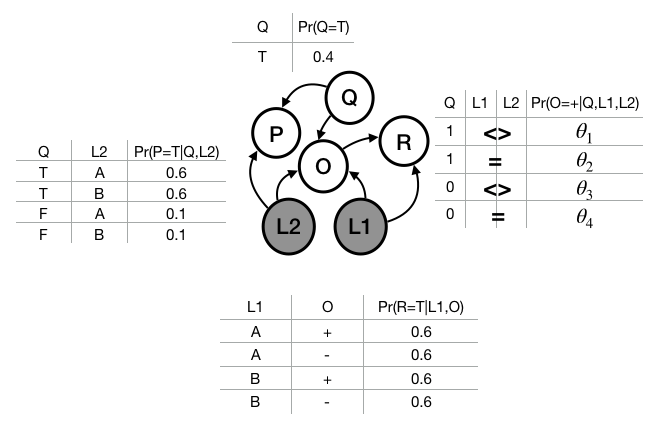
\includegraphics[width=\textwidth]{figs/BN.png}
  \end{minipage}\hfill
  \begin{minipage}[c]{0.45\textwidth}
    \caption{
        \small The model used for generating the datasets. There are four binary random variables, P, Q, O, and R. \textbf{P}: indicates whether or not the employee has high performance; \textbf{Q}: indicates whether or not an employee has high qualification; \textbf{O}: indicates whether or not the colleague submits the positive opinion towards the employee;  \textbf{R}: indicates whether or not the colleague has a positive opinion towards the employee;  \textbf{L1, L2}: indicates the label of the review provider and review receiver (observed).
    } \label{fig:BN}
  \end{minipage}
\end{figure}

We show the effectiveness of FairPSL by performing an empirical evaluation. We investigate two research questions in our experiments:
\begin{description}
\item[Q1] What is the effect of the fairness threshold $\delta$ on the fairness measures $RD/RC/RR$?
\item[Q2] How is decision quality affected by imposing $\delta$-fairness constraints?
\end{description}

Note that although we present the result for specific parameters of the framework in this section, we ran extensive analysis and the results we present are representative. We implemented the MAP inference routines of PSL and FairPSL in Python, using Gurobi-8.1\footnote{\url{www.gurobi.com}} as the backend solver. The FairPSL code, code for the data generator and data is publicly available\footnote{https://github.com/gfarnadi/FairPSL}. 

\subsection{Data generation}
  
We evaluate the FairPSL inference algorithm on synthetic datasets representing the performance review scenario (introduced in Example~\ref{ex:review}). The organization hierarchy is generated synthetically. 
The organization hierarchy generator is parameterized by two numbers: the number of employees in the organization ($n$) and the number of employees managed by each manager ($k$). Each employee is randomly assigned with a label \emph{A} or \emph{B}. An examples organization hierarchy with $n$=50 and $k$=3 is shown in Figure~\ref{fig:hierachy}.

\begin{figure}
  \begin{minipage}[c]{0.3\textwidth}
    \caption{
        \small An example of an organizational hierarchy with five levels and 50 employees with k=3. Each employee either has label A (shown with grey) or B (shown with white).
    }\label{fig:hierachy} 
	\end{minipage} \hfill
    \begin{minipage}[c]{0.7\textwidth}
    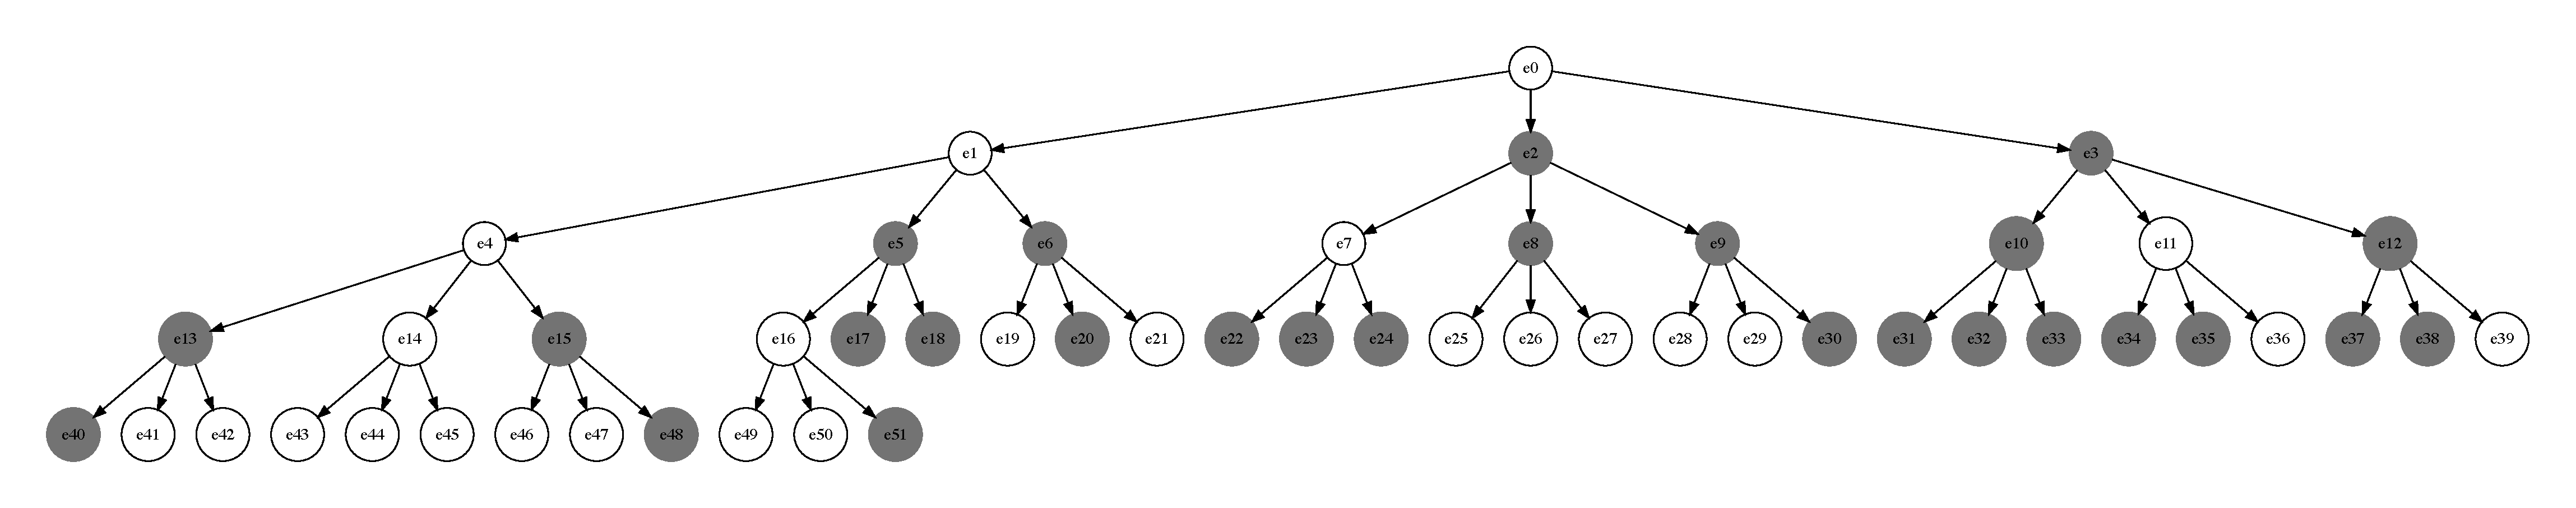
\includegraphics[width=\textwidth]{figs/Uni-hierachy.pdf}
  \end{minipage}
\end{figure}

For each employee, we use the generative model of Figure~\ref{fig:BN} to draw assignments for all the random variables. We assume that only $40\%$ of employees are qualified for promotion and regardless of their labels, employees submit only $60\%$ of their opinions. In addition, due to various personal and environmental factors, only $60\%$ of high quality employees perform well while $10\%$ of low quality employees also perform well regardless of their labels. Note that these numbers are not specific and just chosen for the framework to serve as a representative setting and a proof of concept. The conditional probability table for the opinion variable $O$ is parameterized by four values $(\theta_1, \theta_2, \theta_3, \theta_4)$ which together determine the degree of discrimination against the protected group. Since other parameters in the Bayesian network did not have a direct effect on the degree of discrimination, we fixed them to arbitrary values. 

The results presented in this section are based on an organization hierarchy  with $100$ employees where $k=5$. However, the results of the framework are not sensitive to the settings as we test the framework with various organization sizes ranging from $50$ to $500$ employees and various degree for $k$ ranging from $3$ to $10$. We generated seven datasets given the organization hierarchy using different values for the $\theta$ parameters: $(0.0,1.0,0.0,0.0)$, $(0.33,1.0,0.0,0.0)$, $(0.66,1.0,0.0,0.0)$, $(1.0,1.0,0.0,0.0)$, $(1.0,1.0,0.0,0.33)$, $(1.0,1.0,0.0,0.66)$, $(1.0,1.0,0.0,1.0)$. 
 
In the first three settings the discrimination originates from negative opinions towards qualified outgroup employees. The first setup is an extreme case where the opinion towards outgroup employees is always negative. The discrimination in the last three settings originates from positive opinions towards unqualified ingroup employees. The last setup is an extreme case where the opinion towards ingroup employees is always positive. The fourth setup represent unbiased opinions where employees are treated similarly based on their qualification. 

\paragraph{MAP Inference} We use the model presented in Table~\ref{tab:pslmodel} for MAP inference in PSL and FairPSL (recall that in FairPSL, the $\delta$-fairness constraints corresponding to one of the fairness measures are also added to the model). The observed atoms are $\textit{Manager(m,e)}$, $\textit{PositiveReview(e1,e2)}$ and labels of all employees. The truth values for all other atoms are obtained via MAP inference. We use the truth values obtained for the decision atoms $\textit{ToPromote(e)}$ to compute the fairness measures. We defined the discriminative pattern, and the protected and unprotected groups of this problem in Section~\ref{sec:formulation}.


\subsection{Evaluation results}

\begin{figure}
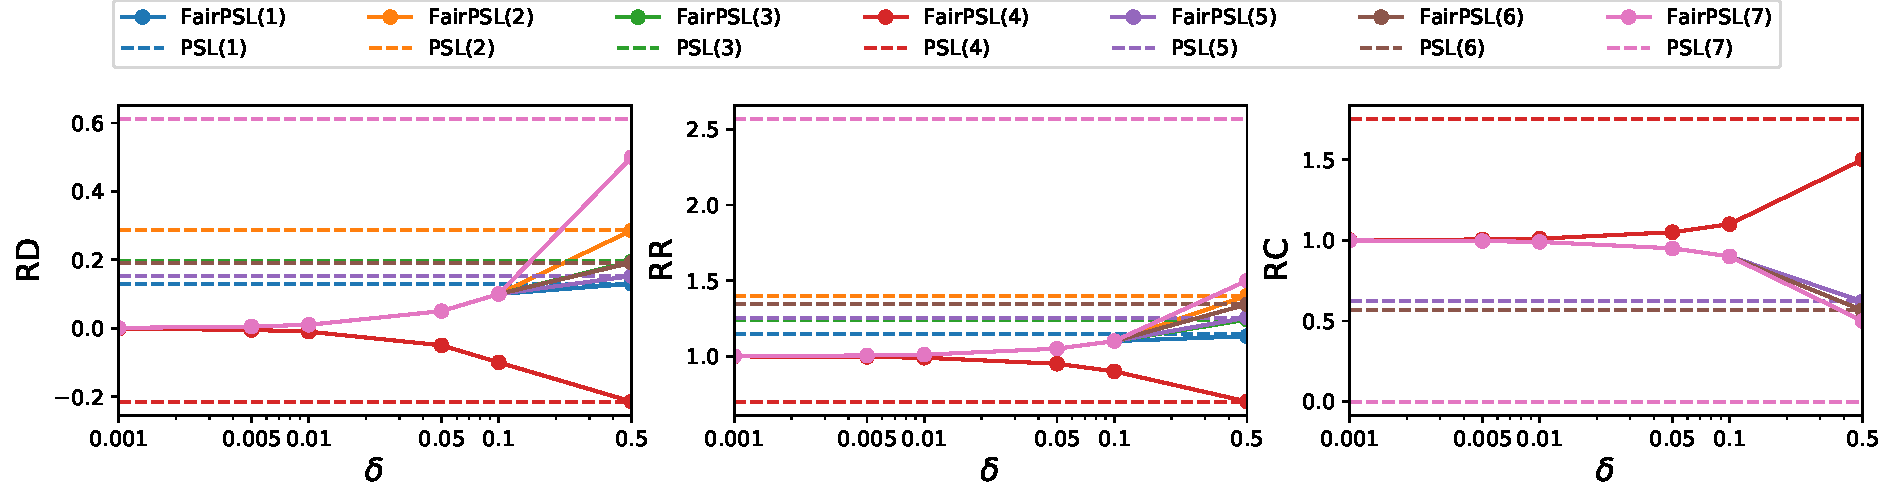
\includegraphics[width=1\linewidth]{figs/results_vis_uni_params.pdf}
\caption{\small Fairness score of predictions obtained by MAP inference of PSL and FairPSL, according to the fairness measures \emph{RD}, \emph{RR}, and \emph{RC}. The labels of datasets are mentioned with parenthesis next to the inference method. The FairPSL values of each measure are obtained by adding the $\delta$-fairness constraint of that measure.\label{fig:results}
}  
\end{figure}

To answer \textbf{Q1}, we run the MAP inference algorithm of PSL and FairPSL on seven synthetic datasets. 
We run the MAP inference of FairPSL multiple times on each dataset: For each of the three fairness measures, we add the corresponding $\delta$-fairness constraint with five thresholds $\{0.001, 0.005, 0.01, 0.05, 0.1, 0.5\}$.

Figure~\ref{fig:results} shows the fairness score of predictions in terms of the three fairness measures. As expected, tighter $\delta$-fairness constraints lead to better scores. Note that the best possible score according to RD is 0, as it computes a difference. Since RR and RC compute ratios, the best possible score according to these measures is 1. In our experiments, with any of these measures, taking $\delta = 0.001$ pushes the score of predictions to its limit.  

The $\delta$-fairness constraints modify the optimization problem of MAP inference by reducing the feasible region to solutions that conform with fairness guarantees. Research question \textbf{Q2} is concerned with the effect of this reduction on the accuracy of predictions. Note that decision quality is the same as the accuracy of predictions. To answer this question, we compare the inferred values for the decision atoms \textit{ToPromote(e)} against their actual values. These values are extracted from the known values of \textit{IsQualified(e)} according to rules 11 and 12 in Table~\ref{tab:pslmodel}. Figure~\ref{fig:accuracy} shows the area under the curve of the receiver operating characteristic~(AUC) of predicting the decision variable in three groups, namely the protected group, the unprotected group (i.e., promotion of the employees who have in-group managers), and all employees. By doing so, we make sure that our fairness constraints do not propagate bias towards either of the populations. Since the results of FairPSL with $\delta$-fairness constraints RR and RC are very similar to the results of RD, we only report the latter here.


\begin{figure}
    \centering
    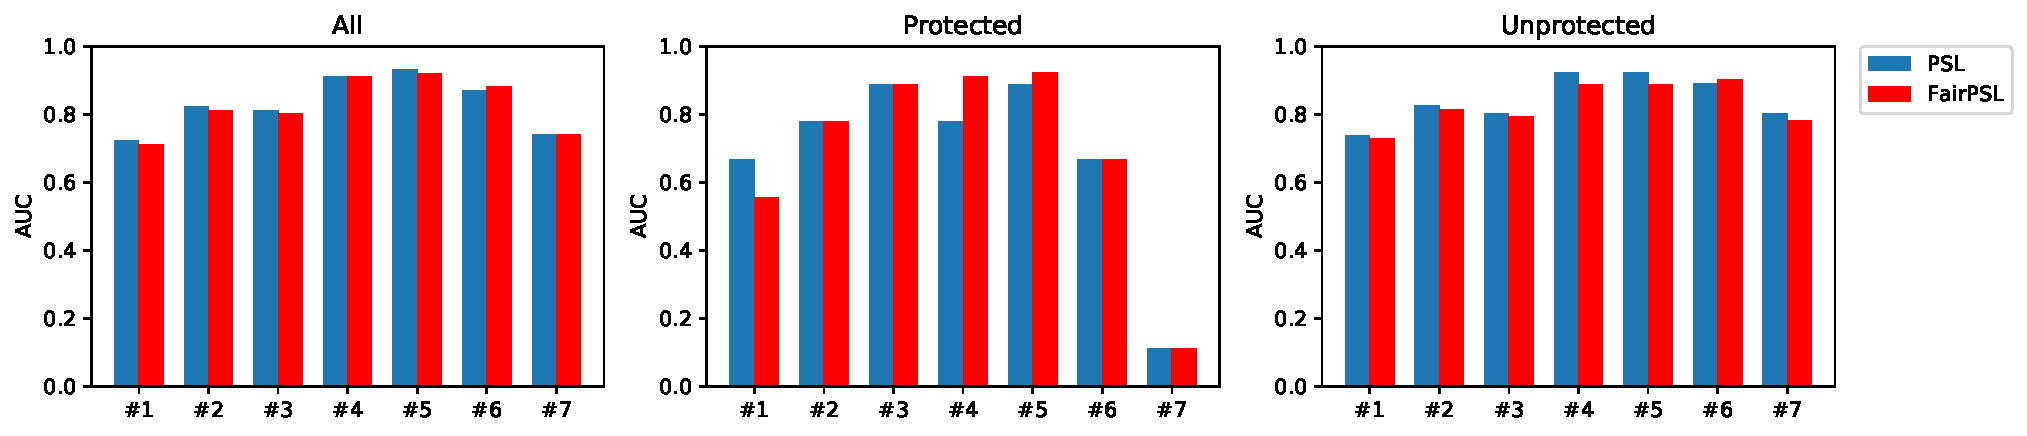
\includegraphics[width=\textwidth]{figs/roc.pdf}
    \caption{\small AUC score of predictions for truth values of unknown atoms \textit{ToPromote(e)} using MAP inference of PSL and FairPSL with $\delta$-fairness constraints $RD$ with $\delta=0.001$.}
    \label{fig:accuracy}
\end{figure}

According to Figure~\ref{fig:accuracy}, the results of both PSL and FairPSL in all seven datasets are close to each other. Note that although fairness may impose a cost in terms of overall accuracy, FairPSL often improves the accuracy of the protected class. Sometimes the overall predictions of FairPSL are even slightly better than PSL (e.g., dataset 6 and 7). As expected, the accuracy of the fourth setting where the opinions are unbiased are similar in both PSL and FairPSL. We observe that prediction of MAP inference for both FairPSL and PSL are similar, thus, in these settings at least, FairPSL guarantees fairness without hurting accuracy. Further investigation is required on the effect of the various ranges of discrimination (i.e., $\theta_1$, $\theta_2$, $\theta_3$, $\theta_4$) on the prediction results of FairPSL.



We also generate various types of organizations in which labels are not uniformly distributed, e.g., one population only occurs at the bottom levels of an organization. While we did not observe any differences in the behavior of our method with respect to accuracy and fairness measure, we found that the degree of discrimination is higher in such organizations. Further investigations on the structure of an organization on discrimination is an interesting direction for future research. 

\section{Conclusion and Future Directions}
\label{sec:conclusion}
Many applications of AI and machine learning affect peoples' lives in important ways. While there is a growing body of work on fairness in AI and ML, it assumes an individualistic notion of fairness.   In this paper, we have proposed a general framework for relational fairness which includes both a rich language for defining discrimination patterns and an efficient algorithm for performing inference subject to fairness constraints. We show our approach enforces fairness guarantees while preserving the accuracy of the predictions. 

There are many avenues for expanding on this work. For example, here we assumed that the discriminative pattern is given, however an automatic mechanism to extract discriminatory situations hidden in a large amount of decision records is an important and required task. Discrimination discovery has been studied for attribute-based fairness~\cite{pedreschi2013discovery}. An interesting next step is discrimination pattern discovery in relational data.

\section*{Acknowledgements}
This work is supported by the National Science Foundation under Grant Numbers CCF-1740850 and IIS-1703331. Golnoosh Farnadi and Behrouz Babaki are  supported by postdoctoral scholarships from IVADO through the Canada First Research Excellence Fund (CFREF) grant.

\begin{thebibliography}{10}
\itemsep=1pt 
\begin{small}

\bibitem{EUlaw}
European union legislation. (a) racial equality directive, 2000; (b) employment
  equality directive, 2000; (c) gender employment directive, 2006; (d) equal
  treatment directive (proposal), 2008.

\bibitem{UKlaw}
{UK} legislation. (a) sex discrimination act, 1975, (b) race relation act,
  1976.

\bibitem{USlaw}
United nations legislation. (a) universal declaration of human rights, 1948,
  (c) convention on the elimination of all forms of racial discrimination,
  1966, (d) convention on the elimination of all forms of discrimination
  against women, 1979.

\bibitem{alshukaili:iswc16}
Duhai Alshukaili, Alvaro A.~A. Fernandes, and Norman~W. Paton.
\newblock Structuring linked data search results using probabilistic soft
  logic.
\newblock In {\em International Semantic Web Conference {(1)}}, volume 9981 of
  {\em Lecture Notes in Computer Science}, pages 3--19, 2016.

\bibitem{bach:jmlr17}
Stephen~H. Bach, Matthias Broecheler, Bert Huang, and Lise Getoor.
\newblock Hinge-loss markov random fields and probabilistic soft logic.
\newblock {\em Journal of Machine Learning Research}, 18:109:1--109:67, 2017.

\bibitem{barocas2016big2}
Solon Barocas and Andrew~D Selbst.
\newblock Big data's disparate impact.
\newblock {\em California Law Review}, 104:671, 2016.

\bibitem{boyd2014networked}
Danah Boyd, Karen Levy, and Alice Marwick.
\newblock The networked nature of algorithmic discrimination.
\newblock In {\em Data and discrimination: Collected essays}, pages 53--57.
  2014.

\bibitem{brewer1979group}
Marilynn~B Brewer.
\newblock In-group bias in the minimal intergroup situation: A
  cognitive-motivational analysis.
\newblock {\em Psychological bulletin}, 86(2):307, 1979.

\bibitem{brewer2007social}
Marilynn~B Brewer.
\newblock The social psychology of intergroup relations: Social categorization,
  ingroup bias, and outgroup prejudice.
\newblock {\em Social Psychology: Handbook of Basic Principles}, 2007.

\bibitem{chouldechova2017fair2}
Alexandra Chouldechova.
\newblock Fair prediction with disparate impact: {A} study of bias in
  recidivism prediction instruments.
\newblock {\em CoRR}, abs/1703.00056, 2017.

\bibitem{dwork2012fairness3}
Cynthia Dwork, Moritz Hardt, Toniann Pitassi, Omer Reingold, and Richard~S.
  Zemel.
\newblock Fairness through awareness.
\newblock In {\em {ITCS}}, pages 214--226. {ACM}, 2012.

\bibitem{ebrahimi:emnlp16}
Javid Ebrahimi, Dejing Dou, and Daniel Lowd.
\newblock Weakly supervised tweet stance classification by relational
  bootstrapping.
\newblock In {\em {EMNLP}}, pages 1012--1017. The Association for Computational
  Linguistics, 2016.

\bibitem{farnadi2018fairness}
Golnoosh Farnadi, Behrouz Babaki, and Lise Getoor.
\newblock Fairness in relational domains.
\newblock In {\em AAAI/ACM Conference on AI, Ethics, and Society (AIES)}, pages
  108--114. ACM, 2018.

\bibitem{feldman2015certifying2}
Michael Feldman, Sorelle~A. Friedler, John Moeller, Carlos Scheidegger, and
  Suresh Venkatasubramanian.
\newblock Certifying and removing disparate impact.
\newblock In {\em {KDD}}, pages 259--268. {ACM}, 2015.

\bibitem{getoor2007introduction}
Lise Getoor and Ben Taskar.
\newblock {\em {Introduction to Statistical Relational Learning}}.
\newblock MIT press Cambridge, 2007.

\bibitem{hardt2016equality3}
Moritz Hardt, Eric Price, and Nati Srebro.
\newblock Equality of opportunity in supervised learning.
\newblock In {\em {NIPS}}, pages 3315--3323, 2016.

\bibitem{kamishima2011fairness}
Toshihiro Kamishima, Shotaro Akaho, and Jun Sakuma.
\newblock Fairness-aware learning through regularization approach.
\newblock In {\em ICDMW}, pages 643--650. {IEEE} Computer Society, 2011.

\bibitem{kouki:recsys15}
Pigi Kouki, Shobeir Fakhraei, James~R. Foulds, Magdalini Eirinaki, and Lise
  Getoor.
\newblock Hyper: {A} flexible and extensible probabilistic framework for hybrid
  recommender systems.
\newblock In {\em RecSys}, pages 99--106. {ACM}, 2015.

\bibitem{counterfactualfairness}
Matt~J. Kusner, Joshua~R. Loftus, Chris Russell, and Ricardo Silva.
\newblock Counterfactual fairness.
\newblock In {\em {NIPS}}, pages 4069--4079, 2017.

\bibitem{Pedreschi:2012}
Dino Pedreschi, Salvatore Ruggieri, and Franco Turini.
\newblock A study of top-k measures for discrimination discovery.
\newblock In {\em {SAC}}, pages 126--131. {ACM}, 2012.

\bibitem{pedreschi2013discovery}
Dino Pedreschi, Salvatore Ruggieri, and Franco Turini.
\newblock The discovery of discrimination.
\newblock In {\em Discrimination and Privacy in the Information Society},
  volume~3 of {\em Studies in Applied Philosophy, Epistemology and Rational
  Ethics}, pages 91--108. Springer, 2013.

\bibitem{ridgeway2004unpacking}
Cecilia~L Ridgeway and Shelley~J Correll.
\newblock Unpacking the gender system: A theoretical perspective on gender
  beliefs and social relations.
\newblock {\em Gender \& society}, 18(4):510--531, 2004.

\bibitem{sridhar:bioinformatics16}
Dhanya Sridhar, Shobeir Fakhraei, and Lise Getoor.
\newblock A probabilistic approach for collective similarity-based drug-drug
  interaction prediction.
\newblock {\em Bioinformatics}, 32(20):3175--3182, 2016.

\bibitem{verma2018fairness2}
Sahil Verma and Julia Rubin.
\newblock Fairness definitions explained.
\newblock In {\em 2018 IEEE/ACM International Workshop on Software Fairness
  (FairWare)}, pages 1--7. IEEE, 2018.

\bibitem{west2014exploiting}
Robert West, Hristo~S. Paskov, Jure Leskovec, and Christopher Potts.
\newblock Exploiting social network structure for person-to-person sentiment
  analysis.
\newblock {\em {TACL}}, 2:297--310, 2014.

\bibitem{zafar2017parity}
Muhammad~Bilal Zafar, Isabel Valera, Manuel Gomez{-}Rodriguez, Krishna~P.
  Gummadi, and Adrian Weller.
\newblock From parity to preference-based notions of fairness in
  classification.
\newblock In {\em {NIPS}}, pages 228--238, 2017.

\bibitem{zemel2013learning}
Richard~S. Zemel, Yu~Wu, Kevin Swersky, Toniann Pitassi, and Cynthia Dwork.
\newblock Learning fair representations.
\newblock In {\em {ICML} {(3)}}, volume~28 of {\em {JMLR} Workshop and
  Conference Proceedings}, pages 325--333. JMLR.org, 2013.

\end{small}
\end{thebibliography}

\end{document}

\end{article}


\begin{article}
{Report from the Workshop on Common Model Infrastructure, {ACM KDD 2018}}
{Chaitanya Baru}
%\documentclass[11pt,dvipdfm]{article}
\documentclass[11pt]{article}
\usepackage{deauthor,times,graphicx} %required
\usepackage{amsmath,amssymb}
\usepackage{multirow}
\usepackage{algorithm}
\usepackage{algpseudocode}
\usepackage{todonotes}
\usepackage{url}

% \graphicspath{{farnadi/}}

\newtheorem{mydef}{\textbf{Definition}}
\newtheorem{myex}{\textbf{Example}}
\newtheorem{mytheorem}{\textbf{Theorem}}


\begin{document}

\title{A Declarative Approach to Fairness in Relational Domains}
\author{Golnoosh Farnadi$^{1,2}$, Behrouz Babaki$^1$, Lise Getoor$^3$\\
$^1$Polytechnique Montr\'{e}al, $^2$ Mila, $^3$ UC Santa Cruz \\
farnadig@mila.quebec, behrouz.babaki@polymtl.ca, getoor@soe.ucsc.edu}

\maketitle

\begin{abstract}
AI and machine learning tools are being used with increasing frequency for decision making in domains that affect peoples' lives such as employment, education, policing and %loan approval
financial qualifications. These uses raise concerns about biases of algorithmic discrimination and have motivated the development of fairness-aware machine learning. However, existing fairness approaches are based solely on attributes of individuals. In many cases, discrimination is much more complex, and taking into account the social, organizational, and other connections between individuals is important. We introduce new notions of fairness that are able to capture the relational structure in a domain. We use first-order logic to provide a flexible and expressive language for specifying complex relational patterns of discrimination. Furthermore, we extend an existing statistical relational learning framework, probabilistic soft logic~(PSL), to incorporate our definition of relational fairness. We refer to this fairness-aware framework FairPSL. FairPSL makes use of the logical definitions of fairnesss but also supports a probabilistic interpretation. In particular, we show how to perform maximum a posteriori~(MAP) inference by exploiting probabilistic dependencies within the domain while avoiding violations of fairness guarantees. Preliminary empirical evaluation shows that we are able to make both accurate and fair decisions.
\end{abstract}

\section{Introduction}
\label{sec:introduction}

Over the past few years, AI and machine learning have become essential components in operations that drive the modern society, e.g., in financial, administrative, and educational spheres. \emph{Discrimination} happens when qualities of individuals which are not relevant to the decision making process influence the decision. Delegating decision making to an automated process raises questions about discriminating against individuals with certain traits based on biases in the data. This is especially important when the decisions have the potential to impact the lives of individuals, for example, the decisions on granting loans, assigning credit, and employment. 

\emph{Fairness} is defined as the absence of discrimination in a decision making process. The goal of \emph{fairness-aware} machine learning is to ensure that the decisions made by an algorithm do not discriminate against a population of individuals~\cite{feldman2015certifying2,boyd2014networked,hardt2016equality3}. Fairness has been well studied in the social sciences and legal scholarship (for an in-depth review see~\cite{barocas2016big2}), and there is emerging work on fairness-aware ML within the AI and computer science communities. For example, fairness through awareness/Lipschitz property~\cite{dwork2012fairness3}, individual fairness~\cite{zemel2013learning}, statistical parity/group fairness~\cite{kamishima2011fairness}, counterfactual fairness~\cite{counterfactualfairness}, demographic parity/disparate impact~\cite{feldman2015certifying2,chouldechova2017fair2}, preference-based fairness~\cite{zafar2017parity}, and equality of opportunity~\cite{hardt2016equality3}.

The existing work in fairness-aware machine learning is based on a definition of discrimination where a decision is influenced by an \emph{attribute} of an individual. An attribute value upon which discrimination is based (such as gender, race, or religion) is called a \emph{sensitive attribute}. The sensitive attribute defines a population of vulnerable individuals known as the \emph{protected group}. A fair decision-making process treats the protected group the same as the \emph{unprotected group}. 

However, in many social contexts, discrimination is the result of complex interactions and can not be described solely in terms of attributes of an individual. For example, consider an imaginary scenario in an organization in which younger female workers who have older male supervisors have lower chances of promotion than their male counterparts.\footnote{Of course, many other patterns may be possible: female bosses may promote female subordinates and discriminate against male workers, or male bosses may promote female employees.  Our goal is to provide a general framework which is able to describe arbitrarily complex discrimination patterns.} 
 This discrimination pattern involves two attributes of the individual (gender and age), a relationship with another individual (supervisor), and two attributes of the second individual. Addressing such complex cases poses two challenges. First, the concepts of discrimination and fairness need to be extended to capture not only attributes of individuals but also the relationships between them. Second, a process is required that ensures that fair decisions are made about individuals who are affected by such patterns. In this paper we address both of these challenges.
We use first-order logic (FOL) to extend the notion of fairness to the relational setting. FOL is an expressive representation for relational problems which is also widely used for learning in relational domains. Moreover, we extend an existing framework for statistical relational learning~\cite{getoor2007introduction} called probabilistic soft logic (PSL)\footnote{http://psl.linqs.org/}~\cite{bach:jmlr17}. PSL combines logic and probability for learning and reasoning over uncertain relational domains. One of the most common reasoning tasks in PSL is called maximum a posteriori (MAP) inference, which is performed by finding the most probable truth values for unknowns over a set of given evidence. We develop a new MAP inference algorithm which is able to maximize the a posteriori values of unknown variables \emph{subject to} fairness guarantees. An early version of this paper which this work builds upon and extends appeared in~\cite{farnadi2018fairness}.

\looseness-1
Our contributions are as follows: 1) we propose fairness-aware machine learning for the relational setting; 2) we extend PSL into a fairness-aware framework called FairPSL which can represent the logical definition of fairness; 3) we develop a new MAP inference algorithm which is able to maximize the posteriori values of unknown variables \emph{subject to} fairness guarantees; 4) we empirically evaluate our proposed framework on synthetic data. 

\section{Motivation}
\label{sec:motivation}

Discrimination in social contexts have been studied in the field of social psychology~\cite{brewer2007social,brewer1979group,ridgeway2004unpacking}. There is a large literature on various aspects of relational bias in social contexts such as \emph{in-group-out-group bias}, \emph{gender bias}, and \emph{ethnicity-based favoritism} that can result in discrimination. 
As an example, consider gender bias in the workplace that reflects stereotypically masculine criteria and male-based favoritism. Such gender bias 
typically places women in lower positions and negatively impacts their opportunities. Further, lack of women in leadership positions may affect the promotion of women and results in a glass ceiling that keeps women from rising beyond a certain level in the hierarchy. This scenario shows that considering  protected attributes such as gender is not always sufficient to detect the source of bias and avoid discrimination, one also has to consider the relational information, in this case the organization hierarchy. Note that this can be generalized to any ingroup/outgroup scenario where the sensitive attribute could be race, religion, age, marital-status, etc.

The existing work on designing fair algorithms in machine learning exclusively focuses on \emph{attribute-based fairness}, which is based on the following assumptions: First, there is an assumption that the individuals (sometimes referred to as units or entities) are independent and described by simple attribute vectors. Second, the group for which one wishes to ensure fairness (known as the \emph{protected group}) is defined on the basis of some attribute values. Finally, there is a decision that is associated with each individual, and the goal is to ensure that members of the protected group are subject to a fair decision (we discuss different fairness measures in Section~\ref{sec:fairnessmeasure}).  We illustrate  attribute-based fairness in the following example. 

\begin{myex}[Loan Processing]
\label{ex:loan}
A bank bases its decisions about granting a loan on attributes of the applicant. The goal is to decide whether to grant a loan to an applicant using a predictive model. The bank needs to ensure that the obey fair lending practices and ensure that gender, race, sexual orientation of applicants has no influence on the decision. In this scenario, the protected group is the historically disadvantaged applicants.  
\end{myex}
The current fairness-aware machine learning techniques are not capable of modeling relations and hence cannot be used to make the decision making model fair. However, in many decision making scenarios, especially in social and organizational settings, the domain is relational, and the protected group itself might be best represented using a relational definition. We illustrate this setting in the following scenario:
\begin{myex}[Performance Review]
\label{ex:review}
Consider an organization where decisions about the promotion of employees is based on two criteria: 1) an objective performance measure, and 2) the opinion of their direct and indirect managers above them. The opinions are inferred from the performance reviews which are collected periodically. Not every manager can submit a review for all its subordinates, this is especially the case for top-level managers who have a large number of subordinates. Hence, the opinions of managers are collectively inferred from the opinions of their sub-ordinates. However, some employees may be biased, and judge other employees unfavorably, by favoring employees who are similar to themselves (same gender, race, religion, etc.) over employees who are dissimilar. The organization needs to ensure that promotion of employees do not have any relational bias caused by in-group-out-group favoritism.

\end{myex}
Example~\ref{ex:review} describes a prediction problem over a database that consists of relations between employees. Such prediction tasks are best handled by techniques from the relational learning domain. To ensure fair prediction in such settings, we need to extend the notion of \emph{attribute-based fairness} to \emph{relational fairness}. Throughout this paper, we use the performance review problem as a running example for relational fairness.

\section{Fairness Formalism}
\label{sec:formulation}

A representation that can describe different types of entities and different relationships between them is called relational. In this section, we use first-order logic to define relational fairness. We employ first-order logic as an expressive representation formalism which can represent objects and complex relationships between them. We start by defining an atom:

\begin{mydef}[Atom]
An atom is an expression of the form $P(a_1, a_2, \ldots, a_n)$ where each argument $a_1, a_2,$ $\ldots,$ $a_n$ is either a constant or a variable. The finite set of all possible substitutions of a variable to a constant for a particular variable $a$ is called its \textit{domain} $D_{a}$. If all variables in $P(a_1, a_2, \ldots, a_n)$ are substituted by some constant from their respective domain, then we call the resulting atom a \textit{ground atom}. 
\end{mydef}

\begin{myex}
In our loan processing problem (Example~\ref{ex:loan}), we can represent applicants' attributes by atoms. For instance, atom $Female(v)$ indicates whether or not applicant $v$ is female. Similarly, we can represent relations with atoms. In the performance review problem in Example~\ref{ex:review} the atom $Manager(m,e)$ indicates whether or not employee $m$ is a direct or indirect manager of employee $e$.
\end{myex}

The relational setting provides the flexibility to express complex definitions with formulae.

\begin{mydef}[Formula] 
A formula is defined by induction: every atom is a formula. If $\alpha$ and $\beta$ are formulae, then $\alpha \vee \beta$, $\alpha \wedge \beta$, $\neg \alpha$, $\alpha \rightarrow \beta$ are formulae. If $x$ is a variable and $\alpha$ is a formula, then the quantified expressions of the form $\exists x$ $\alpha$ and $\forall x$ $\alpha$ are formulae.    
\end{mydef}

To characterize groups of individuals based on a formula, we define the notion of \emph{population}.

\begin{mydef}[Population]
We denote formula $F$ which has only one free variable $v$ (i.e., other variables in $F$ are quantified) by $F[v]$. The population defined by $F[v]$ is the set of substitutions of $v$ for which $F[v]$ holds.   
\end{mydef}


\begin{myex}
\label{ex:disformula}
Consider the formula $F[v] := \forall u, \, \textit{Manager}(u,v) \rightarrow \neg \textit{SameGroup}(u, v)$. The population specified by this formula is the set of individuals all of whose managers belong to a group different from theirs. 
\end{myex}

The truth value of a formula is derived from the truth value of atoms that it comprises, according to the rules of logic. Each possible assignment of truth values to ground atoms is called an \emph{interpretation}. 


\begin{mydef}[Interpretation]
An interpretation $I$ is a mapping that associates a truth value $I(P)$ to each ground atom $P$. For Boolean truth values, $I$ associates true to 1 and false to 0 truth values. For soft logic (see Definition~\ref{def:softlogic}) $I$ maps each ground atom $P$ to a truth value in interval $[0, 1]$.
\end{mydef}

In attribute-based fairness, it is assumed that there is a certain attribute of individuals, i.e, the sensitive attribute,  that we do not want to affect a decision. Gender, race, religion and marital status are examples of sensitive attributes. Discrimination has been defined in social science studies as a treatment in favor or against a group of individuals given their sensitive attribute. This group of individuals is the protected group. 

In a relational setting, both the sensitive attributes of an individual and their participation in various relations may have an undesired effect on the final decision. We characterize the protected group in a relational setting by means of a population. In practice, we are often interested in maintaining fairness for a specific population such as applicants, students, employees, etc. This population is then partitioned into the protected and unprotected groups. We define a \emph{discriminative pattern} which is a pair of formulae to capture these groups: 1) $F_1[v]$: to specify the difference between the protected and unprotected groups and 2) $F_2[v]$: to specify the population over which we want to maintain fairness. 

\begin{mydef}[Discriminative pattern]
A discriminative pattern is a pair $\textit{DP}[v]:=(F_1[v], F_2[v])$ , where $F_1[v]$ and $F_2[v]$ are formulae.
\end{mydef}

\begin{myex}
\label{ex:pattern}
The two formulae in the discrimination pattern $\textit{DP}[v]:= \big((\forall u, \,  \textit{Manager}(u,v) \rightarrow  \neg \textit{SameGroup}(u, v)),$ $\textit{Employee}(v)\big)$ specify two populations, namely all employees and those employees who belong to a group different from their managers.
\end{myex}

Given the definition of the discriminative pattern, we have a rich language to define the scope of the protected and unprotected groups in a relational setting.

\begin{mydef}[Protected group] Given an interpretation $I$, the protected group is a population of the form:
{$$PG :=\{ v : F_1[v] \wedge F_2[v]\}$$}
which is defined as the set of all instances hold for variable $v$ for which $F_1[v] \wedge F_2[v]$ is true under interpretation $I$, that is, $I(F_1[v] \wedge F_2[v]) = 1$. 
Similarly, the \emph{unprotected group} is a population of the form: 
{$$UG := \{ v : \neg F_1[v] \wedge  F_2[v]\}$$}
which is defined as the set of all instances hold for variable $v$ 
for which $I(\neg F_1[v] \wedge F_2[v]) = 1$. 
\end{mydef}

\begin{myex}
The protected group of the discrimination pattern specified in Example~\ref{ex:pattern} is {$PG := \big\{ v : \big(\forall u, \,$ $ \textit{Manager}(u, v) \rightarrow \neg \textit{SameGroup}(u, v)\big) \wedge \textit{Employee}(v) \big\}$} and the unprotected group is {$UG :=  \big\{ v:  \big(\exists u, \, \textit{Manager}(u,v) \wedge \textit{SameGroup}(u, v)\big) \wedge \textit{Employee}(v) \big\}$}. This means our protected group is the set of employees belonging to a group different from their managers,
and our unprotected group consists of other employees. 
\end{myex}

Discrimination is defined in terms of a treatment or decision that distinguishes between the protected and unprotected groups. Here we define the \emph{decision} atom.
\begin{mydef}[Decision atom] A decision atom $d(v)$ is an atom containing exactly one variable $v$ that specifies a decision affecting the protected group which is defined either by law or end-user.
\end{mydef}
\begin{myex}
The decision atom ${\textit ToPromote}(v)$ indicates whether or not $v$ receives a promotion.
\end{myex}

Note that the fairness formulation in this section is designed for the relational setting, however relational fairness subsumes the attribute-based fairness such that: a sensitive attribute is defined by an atom with one argument and $F_2[v]$ in discrimination pattern is $\textit{Applicant}(v)$. For example, discrimination pattern of our loan processing problem in Example~\ref{ex:loan} is of the form $\textit{DP} := ( \textit{Female}(v), \textit{Applicant}(v))$ that denotes female applicants as the protected group (i.e., $PG :=  \{ v: \textit{Female}(v) \}$) and male applicants as the unprotected group (i.e., $UG := \{ v: \neg \textit{Female}(v)\}$).


\section{Fairness Measures}
\label{sec:fairnessmeasure}

Over the past few years, many fairness measures have been introduced~\cite{verma2018fairness2}. An important class of these measures are \emph{group fairness} measures which quantify the inequality between different subgroups. Some of the most popular measures in this class include \emph{equal opportunity}, \emph{equalized odds}, and \emph{demographic parity}~\cite{hardt2016equality3}. In this paper we restrict our focus to the latter. In an attribute-value setting, demographic parity means that the decision should be independent of the protected attributes. Assume that binary variables $A$ and $C$ denote the decision and protected attributes, and the preferred value of $A$ is one. Demographic parity requires that:

\begin{equation*}
    P(A=1 | C=0) = P(A=1 | C=1)
\end{equation*}

We will now generalize this measure to the relational setting using the notations defined in Section~\ref{sec:formulation}. Let $a$ and $c$ denote the counts of denial (i.e., negative decisions) for protected and unprotected groups, and $n_{1}$ and $n_{2}$ denote their sizes, respectively. Given the decision atom $d(v)$, discriminative pattern $\textit{DP}(F_1[v], F_2[v])$, and interpretation $I$, these counts are computed by the following equations: 
{
\begin{flalign}
    & a \equiv \sum_{v \in D_v} I\big( \neg d(v) \wedge  F_1[v] \wedge F_2[v]) \label{eq:a}\\
    & c \equiv \sum_{v \in D_v} I\big( \neg d(v) \wedge  \neg F_1[v] \wedge  F_2[v]) \label{eq:c}\\
    & n_{1} \equiv \sum_{v \in D_v} I\big(F_1[v] \wedge F_2[v]) \label{eq:n1}\\
    & n_{2} \equiv \sum_{v \in D_v} I\big(\neg F_1[v] \wedge  F_2[v]) \label{eq:n2}
\end{flalign}}
The proportions of denying for protected and unprotected groups are $p_1 = \frac{a}{n_1}$ and $p_2 = \frac{c}{n_2}$, respectively. There are a number of data-driven measures~\cite{Pedreschi:2012} which quantify demographic disparity and can be defined in terms of $p_1$ and $p_2$:
\begin{itemize}
    \item \textbf{Risk difference}: $RD = p_1 - p_2$, also known as absolute risk reduction. 
    \item \textbf{Risk Ratio}: $RR = \frac{p_1}{p_2}$, also known as relative risk. 
    \item \textbf{Relative Chance}: $RC = \frac{1 - p_1}{1 - p_2}$ also, known as selection rate.
\end{itemize}
These measures have been used in the legal systems of European Union, UK, and US~\cite{EUlaw,UKlaw,USlaw}. Notice that RR is the ratio of the proportion of benefit denial between the protected and unprotected groups, while RC is the ratio of the proportion of benefit granted. Finally, we introduce the notion of $\delta$-fairness.

\begin{mydef}[$\delta$-fairness]
If a fairness measure for a decision making process falls within some $\delta$-window, then the process is \emph{$\delta\text{-fair}$}. Given $0 \leq \delta \leq 1$, the  $\delta$-windows for measures RD/RR/RC are defined as:
{\begin{flalign*}
	     - \delta \leq &RD \leq \delta \\
	     1- \delta \leq &RR \leq 1+ \delta\\
	     1- \delta \leq &RC \leq 1+ \delta
	\end{flalign*}}
\end{mydef}

To overcome the limitations of attribute-based fairness, we introduce a new statistical relational learning~(SRL) framework~\cite{getoor2007introduction} suitable for modelling fairness in relational domain. In the next section, we review probabilistic soft logic~(PSL). We then extend PSL with the definition of relational fairness introduced above in Section~\ref{sec:fairMAP}. Our fairness-aware framework, ``FairPSL'', is the first SRL framework that performs fair inference. 

\section{Background: Probabilistic Soft Logic}
\label{sec:psl}

In this section, we review the syntax and semantics of PSL, and in the next section we extend MAP inference in PSL with fairness constraints to define MAP inference in FairPSL.

PSL is a probabilistic programming language for defining hinge-loss Markov random fields~\cite{bach:jmlr17}. Unlike other SRL frameworks whose atoms are Boolean, atoms in PSL can take continuous values in the interval $[0,1]$. PSL is an expressive modeling language that can incorporate domain knowledge with first-order logical rules and has been used successfully in various domains, including bioinformatics~\cite{sridhar:bioinformatics16}, recommender systems~\cite{kouki:recsys15}, natural language processing~\cite{ebrahimi:emnlp16}, information retrieval~\cite{alshukaili:iswc16}, and social network analysis~\cite{west2014exploiting}, among many others. 
 
A PSL model is defined by a set of first-order logical rules called \emph{PSL rules}.

\begin{mydef} [PSL rule] a PSL rule $r$ is an expression of the form:
{\begin{equation}
\lambda_{r}: T_1 \land T_2 \land \ldots \land T_w \rightarrow H_1 \vee H_2 \vee \ldots \vee H_l
\end{equation}}

where { $T_1, T_2, \ldots, T_w, H_1, H_2, \ldots, H_l$} are atoms or negated atoms and { $\lambda_{r} \in \mathbb{R}^{+} \cup \infty$} is the weight of the rule $r$.  We call { $T_1 \land T_2 \land \ldots \land T_w$} the body of $r$ ($r_{body}$), and { $H_1 \vee H_2 \vee \ldots \vee H_l$} the head of $r$ ($r_{head}$).
\end{mydef}


Since atoms in PSL take on continuous values in the unit interval $[0,1]$, next we define soft logic to calculate the value of the PSL rules under an interpretation $I$.

\begin{mydef}[Soft logic]
\label{def:softlogic}
The ({$\tilde{\wedge}$}) and ({$\tilde{\vee}$}) and negation ({$\tilde{\neg}$}) are defined as follows. For {$m, n \in [0,1]$} we have: {$m \tilde{\wedge} n = \max(m+n -1, 0)$}, {$m \tilde{\vee} n = \min(m+n , 1)$} and {$\tilde{\neg} m = 1 - m$}. The $\, \tilde{} \,$ indicates the relaxation over Boolean values.
\end{mydef}

The probability of truth value assignments in PSL is determined by the rules' \emph{distance to satisfaction}.

\begin{mydef}[The distance to satisfaction]
The distance to satisfaction $d_{r}(I)$ of a rule $r$ under an interpretation $I$ is defined as:
{
\begin{equation}
d_{r}(I) = \max\{0, I(r_{body})-I(r_{head})\}
\end{equation}}
\end{mydef}

By using Definition~\ref{def:softlogic}, one can show that the closer the interpretation of a grounded rule $r$ is to 1, the smaller its distance to satisfaction. A PSL model induces a distribution over interpretations $I$. Let $R$ be the set of all grounded rules, then the probability density function is:
{
\begin{equation}
f(I) ={\frac{1}{Z}} \exp[-\sum_{r\in R} \lambda_{r}(d_{r}(I))^p]
\label{eq:potential}
\end{equation}
}
\noindent where { $\lambda_{r}$} is the weight of rule $r$, {
$Z = \int_{I} \exp[ -\sum_{r\in R} \lambda_{r}(d_{r}(I))^p]$
} is a normalization constant, and { $p \in \{1,2\}$} provides a choice of two different loss functions, $p=1$ (i.e., linear), and $p=2$ (i.e, quadratic). These probabilistic models are instances of hinge-loss Markov random fields~(HL-MRF)~\cite{bach:jmlr17}. The goal of maximum a posteriori (MAP) inference is to find the most probable truth assignments $I_{\textit{MPE}}$ of unknown ground atoms given the evidence which is defined by the interpretation $I$. Let $X$ be all the evidence, i.e., $X$ is the set of ground atoms such that $\forall x \in X, I(x)$ is known, and let $Y$ be the set of ground atoms such that $\forall y \in Y, I(y)$ is unknown. Then we have
{
\begin{equation}
I_{\textit{MAP}}(Y) = \textit{arg}\max_{I(Y)} P(I(Y)|I(X))
\end{equation}}
Maximizing the density function in Equation~\ref{eq:potential} is equivalent to minimizing the weighted sum of the distances to satisfaction of all rules in PSL. 

\begin{table*}[t]
    \centering
    \begin{tabular}{|lll|}
    \hline
    &&\\
    $R1$ & $\lambda_1$ &: $\textit{IsQualified}(e) \rightarrow \textit{HighPerformance}(e)$ \\
    $R2$ & $\lambda_1$ &: $\neg \textit{IsQualified}(e) \rightarrow \neg \textit{HighPerformance}(e)$ \\
    $R3$ & $\infty$ &: $\textit{PositiveReview}(e1, e2) \rightarrow \textit{PositiveOpinion}(e1, e2)$ \\
    $R4$ & $\infty$ &: $\neg \textit{PositiveReview}(e1, e2) \rightarrow \neg \textit{PositiveOpinion}(e1, e2)$ \\
    $R5$ & $\lambda_1$ &: $\textit{PositiveOpinion}(e1, e2) \wedge \textit{Manager}(m, e1) \rightarrow \textit{PositiveOpinion}(m, e2)$ \\
    $R6$ & $\lambda_1$ &: $\neg \textit{PositiveOpinion}(e1, e2) \wedge \textit{Manager}(m, e1) \rightarrow \neg \textit{PositiveOpinion}(m, e2)$ \\
    $R7$ & $\lambda_1$ &: $\textit{PositiveOpinion}(m, e) \wedge \textit{Manager}(m, e) \rightarrow \textit{IsQualified}(e)$ \\
    $R8$ & $\lambda_1$ &: $\neg \textit{PositiveOpinion}(m, e) \wedge \textit{Manager}(m, e) \rightarrow \neg \textit{IsQualified}(e)$ \\
    $R9$ &  $\lambda_1$ &: $\neg \textit{ToPromote}(e)$\\
    $R10$ & $\infty$ &: $\textit{IsQualified}(e) \rightarrow \textit{ToPromote}(e)$ \\
    $R11$ & $\infty$ &: $\neg \textit{IsQualified}(e) \rightarrow \neg \textit{ToPromote}(e)$ \\
    &&\\
    \hline
    \end{tabular}
    \caption{\small A simplified PSL model for the \emph{Performance Reviewing} problem}
    \label{tab:pslmodel}
\end{table*}

\begin{myex}
\label{ex:pslmodel}
The simplified PSL model for the performance reviewing problem in Example\ref{ex:review} is given in Table~\ref{tab:pslmodel}. The goal of MAP inference for this problem is to infer employees to promote. We simplified the model by assigning the same weight to all soft rules (i.e., $\lambda_i= 1$ where $i=\{1,2,5,6,7,8,9\}$). Below we explain the meaning of each rule in the model.

Rule $R1$ indicates that qualified employees have high performance and similarly rule $R2$ expresses that a negative qualification of employees is derived from their low performance. Rules $R5$ and $R6$ presents the propagation of opinion from bottom to top of the organizational hierarchy, i.e., managers have similar opinions towards employees given the opinions of their sub-ordinate managers. And rules $R7$ and $R8$ indicate that the positive/negative opinion of direct/indirect managers derive from the qualification of an employee. Rule $R9$ indicates the prior that not all employees get promoted. We also have four hard constraints (i.e., rules $R3$, $R4$, $R10$ and $R11$) where the weight of the rules are $\infty$. Rules $R3$ and $R4$ indicate that submitted positive/negative reviews should reflect positive/negative opinions. And two rules $R10$ and $R11$ show that a highly qualified employee should get promoted. 
\end{myex}

\section{Fairness-aware PSL (FairPSL)}
\label{sec:fairMAP}

The standard MAP inference in PSL aims at finding values that maximize the conditional probability of unknowns. Once a decision is made according to these values, one can use the fairness measure to quantify the degree of discrimination. A simple way to incorporate fairness in MAP inference is to add the $\delta$-fairness constraints to the corresponding optimization problem.   

Consider risk difference, $\textit{RD}$, where $\textit{RD} \equiv \frac{\mathbf{a}}{n_1} - \frac{\mathbf{c}}{n_2}$. The $\delta$-fairness constraint $-\delta \leq \textit{RD} \leq \delta$ can be encoded as the following constraints:
{\begin{align}
    & n_2 \mathbf{a} - n_1 \mathbf{c} - n_1 n_2 \delta \leq 0 \label{eq:RD1}\\
    & n_2 \mathbf{a} - n_1 \mathbf{c} + n_1 n_2 \delta \geq 0
\end{align}}
Similarly, from $\textit{RR} \equiv \frac{\mathbf{a} / n_1}{\mathbf{c} / n_2}$ and the $\delta$-fairness constraint $1 - \delta \leq \textit{RR} \leq 1 + \delta$ we obtain:
{\begin{align}
    & n_2 \mathbf{a} - (1 + \delta) n_1 \mathbf{c} \leq 0 \\
    & n_2 \mathbf{a} - (1 - \delta) n_1 \mathbf{c} \geq 0
\end{align}}
And finally, $\textit{RC} \equiv \frac{1 - \mathbf{a} / n_1}{1 - \mathbf{c} / n_2}$ and the $\delta$-fairness constraint $1 - \delta \leq \textit{RC} \leq 1 + \delta$ gives:
{ \begin{align}
    & - n_2 \mathbf{a} + (1 + \delta) n_1 \mathbf{c} - \delta n_1 n_2 \leq 0 \\
    & - n_2 \mathbf{a} + (1 - \delta) n_1 \mathbf{c} + \delta n_1 n_2 \geq 0 \label{eq:RC2}
\end{align}}
A primary advantage of PSL over similar frameworks is that its MAP inference task reduces to a convex optimization problem which can be solved in polynomial time. To preserve this advantage, we need to ensure that the problem will remain convex after the addition of $\delta$-fairness constraints. 

\begin{mytheorem}
The following condition is sufficient for preserving the convexity of MAP inference problem after addition of $\delta$-fairness constraints: The formulae $F_1[v]$ and $F_2[v]$ do not contain an atom $y \in Y$ and all atoms in $F_1[v]$ and $F_2[v]$ have values zero or one.
\end{mytheorem}
\begin{proof}
Since $I(F_1[v])$ and $I(F_2[v])$ do not depend on $I(Y)$, the values $n_{1}$ and $n_{2}$ are constants that can be computed in advance. Let us define the sets $D_v^a = \{ v \in D_v : F_1[v] \wedge F_2[v] \, \text{is true} \}$ and $D_v^c = \{ v \in D_v : \neg F_1[v] \wedge F_2[v] \, \text{is true} \}$. Since $F_1[v]$ and $F_2[v]$ can be only zero or one, we can rewrite the equations~\ref{eq:a} and \ref{eq:c} as:
{
\begin{align*}
    & \mathbf{a} = \sum_{v \in D_v^a} I(\neg d(v)) = |D_v^a| - \sum_{v \in D_v^a} I(d(v))\\
    & \mathbf{c} = \sum_{v \in D_v^c} I(\neg d(v)) = |D_v^c| - \sum_{v \in D_v^c} I(d(v))
\end{align*}}
\noindent which indicates that $\mathbf{a}$ and $\mathbf{c}$ can be expressed as linear combinations of variables in the optimization problem. This means that constraints~\ref{eq:RD1}-\ref{eq:RC2} are linear. Hence, addition of these constraints preserves the convexity of the optimization problem. 
\end{proof}

\section{Experiments}
\label{sec:experiment}

\begin{figure}
  \begin{minipage}[c]{0.6\textwidth}
    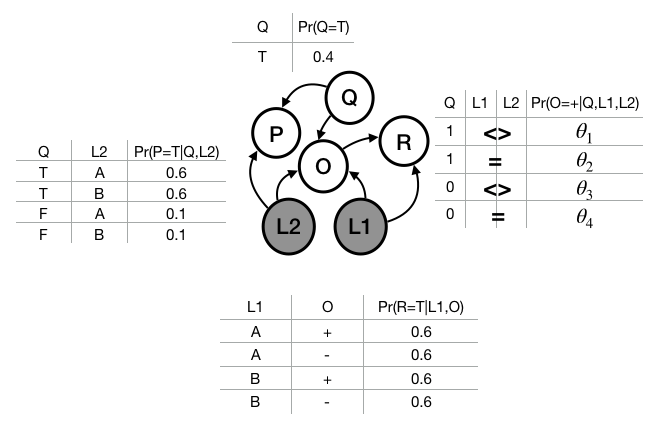
\includegraphics[width=\textwidth]{figs/BN.png}
  \end{minipage}\hfill
  \begin{minipage}[c]{0.45\textwidth}
    \caption{
        \small The model used for generating the datasets. There are four binary random variables, P, Q, O, and R. \textbf{P}: indicates whether or not the employee has high performance; \textbf{Q}: indicates whether or not an employee has high qualification; \textbf{O}: indicates whether or not the colleague submits the positive opinion towards the employee;  \textbf{R}: indicates whether or not the colleague has a positive opinion towards the employee;  \textbf{L1, L2}: indicates the label of the review provider and review receiver (observed).
    } \label{fig:BN}
  \end{minipage}
\end{figure}

We show the effectiveness of FairPSL by performing an empirical evaluation. We investigate two research questions in our experiments:
\begin{description}
\item[Q1] What is the effect of the fairness threshold $\delta$ on the fairness measures $RD/RC/RR$?
\item[Q2] How is decision quality affected by imposing $\delta$-fairness constraints?
\end{description}

Note that although we present the result for specific parameters of the framework in this section, we ran extensive analysis and the results we present are representative. We implemented the MAP inference routines of PSL and FairPSL in Python, using Gurobi-8.1\footnote{\url{www.gurobi.com}} as the backend solver. The FairPSL code, code for the data generator and data is publicly available\footnote{https://github.com/gfarnadi/FairPSL}. 

\subsection{Data generation}
  
We evaluate the FairPSL inference algorithm on synthetic datasets representing the performance review scenario (introduced in Example~\ref{ex:review}). The organization hierarchy is generated synthetically. 
The organization hierarchy generator is parameterized by two numbers: the number of employees in the organization ($n$) and the number of employees managed by each manager ($k$). Each employee is randomly assigned with a label \emph{A} or \emph{B}. An examples organization hierarchy with $n$=50 and $k$=3 is shown in Figure~\ref{fig:hierachy}.

\begin{figure}
  \begin{minipage}[c]{0.3\textwidth}
    \caption{
        \small An example of an organizational hierarchy with five levels and 50 employees with k=3. Each employee either has label A (shown with grey) or B (shown with white).
    }\label{fig:hierachy} 
	\end{minipage} \hfill
    \begin{minipage}[c]{0.7\textwidth}
    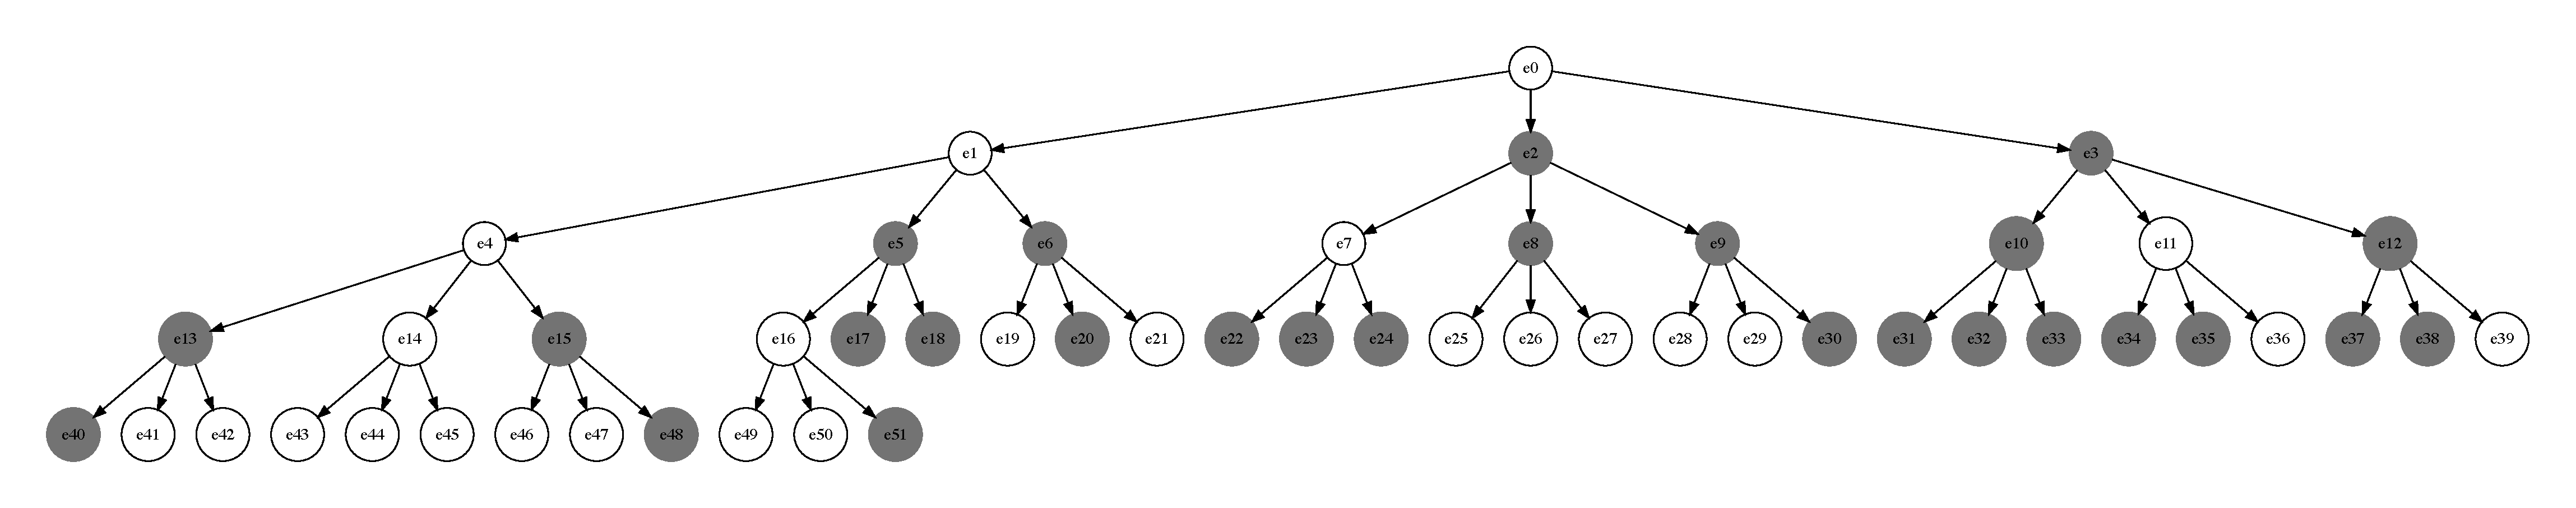
\includegraphics[width=\textwidth]{figs/Uni-hierachy.pdf}
  \end{minipage}
\end{figure}

For each employee, we use the generative model of Figure~\ref{fig:BN} to draw assignments for all the random variables. We assume that only $40\%$ of employees are qualified for promotion and regardless of their labels, employees submit only $60\%$ of their opinions. In addition, due to various personal and environmental factors, only $60\%$ of high quality employees perform well while $10\%$ of low quality employees also perform well regardless of their labels. Note that these numbers are not specific and just chosen for the framework to serve as a representative setting and a proof of concept. The conditional probability table for the opinion variable $O$ is parameterized by four values $(\theta_1, \theta_2, \theta_3, \theta_4)$ which together determine the degree of discrimination against the protected group. Since other parameters in the Bayesian network did not have a direct effect on the degree of discrimination, we fixed them to arbitrary values. 

The results presented in this section are based on an organization hierarchy  with $100$ employees where $k=5$. However, the results of the framework are not sensitive to the settings as we test the framework with various organization sizes ranging from $50$ to $500$ employees and various degree for $k$ ranging from $3$ to $10$. We generated seven datasets given the organization hierarchy using different values for the $\theta$ parameters: $(0.0,1.0,0.0,0.0)$, $(0.33,1.0,0.0,0.0)$, $(0.66,1.0,0.0,0.0)$, $(1.0,1.0,0.0,0.0)$, $(1.0,1.0,0.0,0.33)$, $(1.0,1.0,0.0,0.66)$, $(1.0,1.0,0.0,1.0)$. 
 
In the first three settings the discrimination originates from negative opinions towards qualified outgroup employees. The first setup is an extreme case where the opinion towards outgroup employees is always negative. The discrimination in the last three settings originates from positive opinions towards unqualified ingroup employees. The last setup is an extreme case where the opinion towards ingroup employees is always positive. The fourth setup represent unbiased opinions where employees are treated similarly based on their qualification. 

\paragraph{MAP Inference} We use the model presented in Table~\ref{tab:pslmodel} for MAP inference in PSL and FairPSL (recall that in FairPSL, the $\delta$-fairness constraints corresponding to one of the fairness measures are also added to the model). The observed atoms are $\textit{Manager(m,e)}$, $\textit{PositiveReview(e1,e2)}$ and labels of all employees. The truth values for all other atoms are obtained via MAP inference. We use the truth values obtained for the decision atoms $\textit{ToPromote(e)}$ to compute the fairness measures. We defined the discriminative pattern, and the protected and unprotected groups of this problem in Section~\ref{sec:formulation}.


\subsection{Evaluation results}

\begin{figure}
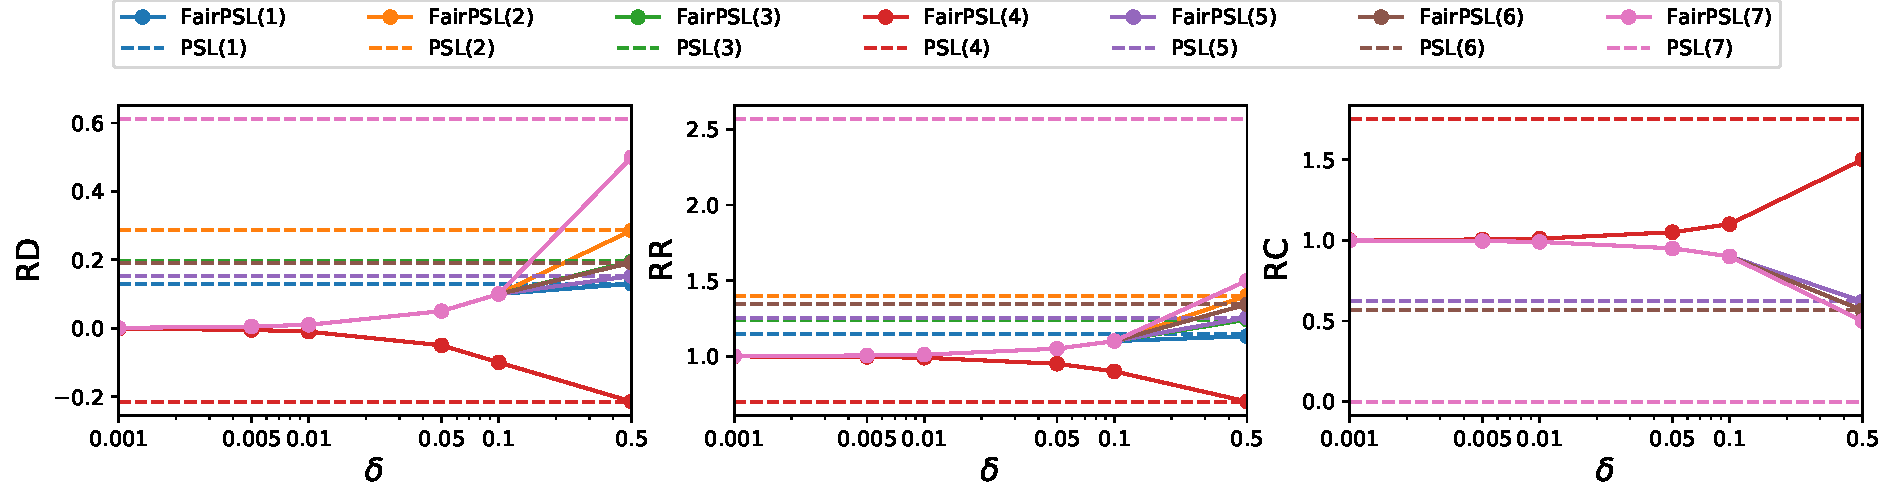
\includegraphics[width=1\linewidth]{figs/results_vis_uni_params.pdf}
\caption{\small Fairness score of predictions obtained by MAP inference of PSL and FairPSL, according to the fairness measures \emph{RD}, \emph{RR}, and \emph{RC}. The labels of datasets are mentioned with parenthesis next to the inference method. The FairPSL values of each measure are obtained by adding the $\delta$-fairness constraint of that measure.\label{fig:results}
}  
\end{figure}

To answer \textbf{Q1}, we run the MAP inference algorithm of PSL and FairPSL on seven synthetic datasets. 
We run the MAP inference of FairPSL multiple times on each dataset: For each of the three fairness measures, we add the corresponding $\delta$-fairness constraint with five thresholds $\{0.001, 0.005, 0.01, 0.05, 0.1, 0.5\}$.

Figure~\ref{fig:results} shows the fairness score of predictions in terms of the three fairness measures. As expected, tighter $\delta$-fairness constraints lead to better scores. Note that the best possible score according to RD is 0, as it computes a difference. Since RR and RC compute ratios, the best possible score according to these measures is 1. In our experiments, with any of these measures, taking $\delta = 0.001$ pushes the score of predictions to its limit.  

The $\delta$-fairness constraints modify the optimization problem of MAP inference by reducing the feasible region to solutions that conform with fairness guarantees. Research question \textbf{Q2} is concerned with the effect of this reduction on the accuracy of predictions. Note that decision quality is the same as the accuracy of predictions. To answer this question, we compare the inferred values for the decision atoms \textit{ToPromote(e)} against their actual values. These values are extracted from the known values of \textit{IsQualified(e)} according to rules 11 and 12 in Table~\ref{tab:pslmodel}. Figure~\ref{fig:accuracy} shows the area under the curve of the receiver operating characteristic~(AUC) of predicting the decision variable in three groups, namely the protected group, the unprotected group (i.e., promotion of the employees who have in-group managers), and all employees. By doing so, we make sure that our fairness constraints do not propagate bias towards either of the populations. Since the results of FairPSL with $\delta$-fairness constraints RR and RC are very similar to the results of RD, we only report the latter here.


\begin{figure}
    \centering
    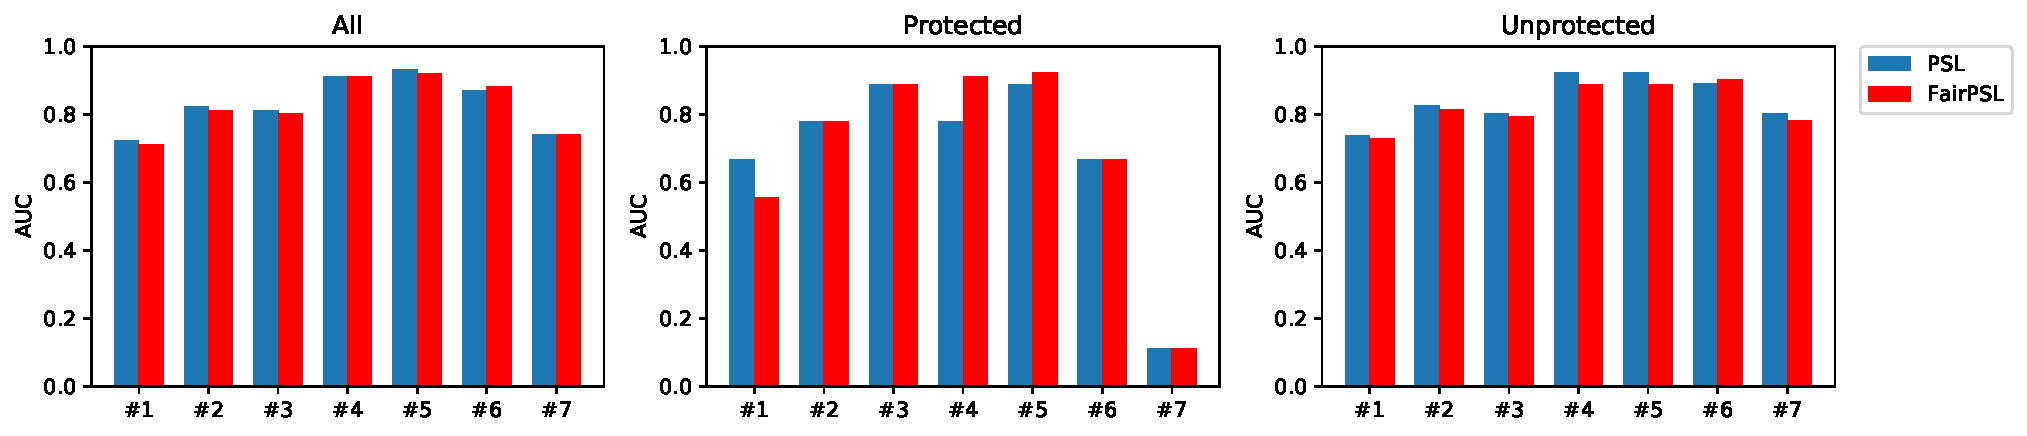
\includegraphics[width=\textwidth]{figs/roc.pdf}
    \caption{\small AUC score of predictions for truth values of unknown atoms \textit{ToPromote(e)} using MAP inference of PSL and FairPSL with $\delta$-fairness constraints $RD$ with $\delta=0.001$.}
    \label{fig:accuracy}
\end{figure}

According to Figure~\ref{fig:accuracy}, the results of both PSL and FairPSL in all seven datasets are close to each other. Note that although fairness may impose a cost in terms of overall accuracy, FairPSL often improves the accuracy of the protected class. Sometimes the overall predictions of FairPSL are even slightly better than PSL (e.g., dataset 6 and 7). As expected, the accuracy of the fourth setting where the opinions are unbiased are similar in both PSL and FairPSL. We observe that prediction of MAP inference for both FairPSL and PSL are similar, thus, in these settings at least, FairPSL guarantees fairness without hurting accuracy. Further investigation is required on the effect of the various ranges of discrimination (i.e., $\theta_1$, $\theta_2$, $\theta_3$, $\theta_4$) on the prediction results of FairPSL.



We also generate various types of organizations in which labels are not uniformly distributed, e.g., one population only occurs at the bottom levels of an organization. While we did not observe any differences in the behavior of our method with respect to accuracy and fairness measure, we found that the degree of discrimination is higher in such organizations. Further investigations on the structure of an organization on discrimination is an interesting direction for future research. 

\section{Conclusion and Future Directions}
\label{sec:conclusion}
Many applications of AI and machine learning affect peoples' lives in important ways. While there is a growing body of work on fairness in AI and ML, it assumes an individualistic notion of fairness.   In this paper, we have proposed a general framework for relational fairness which includes both a rich language for defining discrimination patterns and an efficient algorithm for performing inference subject to fairness constraints. We show our approach enforces fairness guarantees while preserving the accuracy of the predictions. 

There are many avenues for expanding on this work. For example, here we assumed that the discriminative pattern is given, however an automatic mechanism to extract discriminatory situations hidden in a large amount of decision records is an important and required task. Discrimination discovery has been studied for attribute-based fairness~\cite{pedreschi2013discovery}. An interesting next step is discrimination pattern discovery in relational data.

\section*{Acknowledgements}
This work is supported by the National Science Foundation under Grant Numbers CCF-1740850 and IIS-1703331. Golnoosh Farnadi and Behrouz Babaki are  supported by postdoctoral scholarships from IVADO through the Canada First Research Excellence Fund (CFREF) grant.

\begin{thebibliography}{10}
\itemsep=1pt 
\begin{small}

\bibitem{EUlaw}
European union legislation. (a) racial equality directive, 2000; (b) employment
  equality directive, 2000; (c) gender employment directive, 2006; (d) equal
  treatment directive (proposal), 2008.

\bibitem{UKlaw}
{UK} legislation. (a) sex discrimination act, 1975, (b) race relation act,
  1976.

\bibitem{USlaw}
United nations legislation. (a) universal declaration of human rights, 1948,
  (c) convention on the elimination of all forms of racial discrimination,
  1966, (d) convention on the elimination of all forms of discrimination
  against women, 1979.

\bibitem{alshukaili:iswc16}
Duhai Alshukaili, Alvaro A.~A. Fernandes, and Norman~W. Paton.
\newblock Structuring linked data search results using probabilistic soft
  logic.
\newblock In {\em International Semantic Web Conference {(1)}}, volume 9981 of
  {\em Lecture Notes in Computer Science}, pages 3--19, 2016.

\bibitem{bach:jmlr17}
Stephen~H. Bach, Matthias Broecheler, Bert Huang, and Lise Getoor.
\newblock Hinge-loss markov random fields and probabilistic soft logic.
\newblock {\em Journal of Machine Learning Research}, 18:109:1--109:67, 2017.

\bibitem{barocas2016big2}
Solon Barocas and Andrew~D Selbst.
\newblock Big data's disparate impact.
\newblock {\em California Law Review}, 104:671, 2016.

\bibitem{boyd2014networked}
Danah Boyd, Karen Levy, and Alice Marwick.
\newblock The networked nature of algorithmic discrimination.
\newblock In {\em Data and discrimination: Collected essays}, pages 53--57.
  2014.

\bibitem{brewer1979group}
Marilynn~B Brewer.
\newblock In-group bias in the minimal intergroup situation: A
  cognitive-motivational analysis.
\newblock {\em Psychological bulletin}, 86(2):307, 1979.

\bibitem{brewer2007social}
Marilynn~B Brewer.
\newblock The social psychology of intergroup relations: Social categorization,
  ingroup bias, and outgroup prejudice.
\newblock {\em Social Psychology: Handbook of Basic Principles}, 2007.

\bibitem{chouldechova2017fair2}
Alexandra Chouldechova.
\newblock Fair prediction with disparate impact: {A} study of bias in
  recidivism prediction instruments.
\newblock {\em CoRR}, abs/1703.00056, 2017.

\bibitem{dwork2012fairness3}
Cynthia Dwork, Moritz Hardt, Toniann Pitassi, Omer Reingold, and Richard~S.
  Zemel.
\newblock Fairness through awareness.
\newblock In {\em {ITCS}}, pages 214--226. {ACM}, 2012.

\bibitem{ebrahimi:emnlp16}
Javid Ebrahimi, Dejing Dou, and Daniel Lowd.
\newblock Weakly supervised tweet stance classification by relational
  bootstrapping.
\newblock In {\em {EMNLP}}, pages 1012--1017. The Association for Computational
  Linguistics, 2016.

\bibitem{farnadi2018fairness}
Golnoosh Farnadi, Behrouz Babaki, and Lise Getoor.
\newblock Fairness in relational domains.
\newblock In {\em AAAI/ACM Conference on AI, Ethics, and Society (AIES)}, pages
  108--114. ACM, 2018.

\bibitem{feldman2015certifying2}
Michael Feldman, Sorelle~A. Friedler, John Moeller, Carlos Scheidegger, and
  Suresh Venkatasubramanian.
\newblock Certifying and removing disparate impact.
\newblock In {\em {KDD}}, pages 259--268. {ACM}, 2015.

\bibitem{getoor2007introduction}
Lise Getoor and Ben Taskar.
\newblock {\em {Introduction to Statistical Relational Learning}}.
\newblock MIT press Cambridge, 2007.

\bibitem{hardt2016equality3}
Moritz Hardt, Eric Price, and Nati Srebro.
\newblock Equality of opportunity in supervised learning.
\newblock In {\em {NIPS}}, pages 3315--3323, 2016.

\bibitem{kamishima2011fairness}
Toshihiro Kamishima, Shotaro Akaho, and Jun Sakuma.
\newblock Fairness-aware learning through regularization approach.
\newblock In {\em ICDMW}, pages 643--650. {IEEE} Computer Society, 2011.

\bibitem{kouki:recsys15}
Pigi Kouki, Shobeir Fakhraei, James~R. Foulds, Magdalini Eirinaki, and Lise
  Getoor.
\newblock Hyper: {A} flexible and extensible probabilistic framework for hybrid
  recommender systems.
\newblock In {\em RecSys}, pages 99--106. {ACM}, 2015.

\bibitem{counterfactualfairness}
Matt~J. Kusner, Joshua~R. Loftus, Chris Russell, and Ricardo Silva.
\newblock Counterfactual fairness.
\newblock In {\em {NIPS}}, pages 4069--4079, 2017.

\bibitem{Pedreschi:2012}
Dino Pedreschi, Salvatore Ruggieri, and Franco Turini.
\newblock A study of top-k measures for discrimination discovery.
\newblock In {\em {SAC}}, pages 126--131. {ACM}, 2012.

\bibitem{pedreschi2013discovery}
Dino Pedreschi, Salvatore Ruggieri, and Franco Turini.
\newblock The discovery of discrimination.
\newblock In {\em Discrimination and Privacy in the Information Society},
  volume~3 of {\em Studies in Applied Philosophy, Epistemology and Rational
  Ethics}, pages 91--108. Springer, 2013.

\bibitem{ridgeway2004unpacking}
Cecilia~L Ridgeway and Shelley~J Correll.
\newblock Unpacking the gender system: A theoretical perspective on gender
  beliefs and social relations.
\newblock {\em Gender \& society}, 18(4):510--531, 2004.

\bibitem{sridhar:bioinformatics16}
Dhanya Sridhar, Shobeir Fakhraei, and Lise Getoor.
\newblock A probabilistic approach for collective similarity-based drug-drug
  interaction prediction.
\newblock {\em Bioinformatics}, 32(20):3175--3182, 2016.

\bibitem{verma2018fairness2}
Sahil Verma and Julia Rubin.
\newblock Fairness definitions explained.
\newblock In {\em 2018 IEEE/ACM International Workshop on Software Fairness
  (FairWare)}, pages 1--7. IEEE, 2018.

\bibitem{west2014exploiting}
Robert West, Hristo~S. Paskov, Jure Leskovec, and Christopher Potts.
\newblock Exploiting social network structure for person-to-person sentiment
  analysis.
\newblock {\em {TACL}}, 2:297--310, 2014.

\bibitem{zafar2017parity}
Muhammad~Bilal Zafar, Isabel Valera, Manuel Gomez{-}Rodriguez, Krishna~P.
  Gummadi, and Adrian Weller.
\newblock From parity to preference-based notions of fairness in
  classification.
\newblock In {\em {NIPS}}, pages 228--238, 2017.

\bibitem{zemel2013learning}
Richard~S. Zemel, Yu~Wu, Kevin Swersky, Toniann Pitassi, and Cynthia Dwork.
\newblock Learning fair representations.
\newblock In {\em {ICML} {(3)}}, volume~28 of {\em {JMLR} Workshop and
  Conference Proceedings}, pages 325--333. JMLR.org, 2013.

\end{small}
\end{thebibliography}

\end{document}

\end{article}


\fi

\end{articlesection}

%\begin{newssection}{TCDE Election}
%
% there will be other letters- and a blank page will appear in your document
% but the special issue part will be fine
%
%\begin{news}{Letter from the Editor-in-Chief}
%{David Lomet}{Microsoft Corporation}
%\documentclass[11pt]{article} 

\usepackage{deauthor,times,graphicx}
%\usepackage{url}
\usepackage{hyperref}

\begin{document}

\subsection*{ICDE 2018}

Repeating my comment from the last issue-

The IEEE International Conference on Data Engineering will be held in April 14-19, 2018 in Paris, France.  This is the flagship conference of the Computer Society's Technical Committee on Data Engineering.  It is a great conference, at a great location.  What could possibly be better than April in Paris at ICDE!  I am attending and hope to see you there.

\subsection*{About the Bulletin}

This March current issue marks the end of editorial tenure for the Bulletin's current set of editors.  So it is once again time for me to pat myself on the back.  This current set, Tim Kraska, Tova Milo, and Haixun Wang, continue my outstanding success (he says modestly) in finding and choosing great editors.  All three have done truly fine jobs at producing issues that bring to our readers surveys of the latest work in very current areas. The success of the Bulletin depends on great issue editors.  I want to thank Tim, Tova, and Haixun for being exactly that with the fine jobs that they have done.  There was unexpected ``scrambling" over the past two years, so I want to thank them also for their flexibility in coping with this.  


\subsection*{The Current Issue}

Don't you get tired of someone shouting ``FAKE NEWS!".  Or perhaps even worse, being exposed to fake news before it has been labeled as such?  Our political conversations seem increasingly to include many variations of ``fake news" and discussions about which news is fake.  ``Sad." So where am I going with this?

The database world has been working on a key aspect of this problem for many years.  The technical area is called ``data provenance".  And it addresses the problem of where information comes from and how it impacts the subsequent processing of data and the reported results.  The June, 2010 issue was the last one on provenance.  And seven years is a long time in an active technical area, especially an area as important as this.

The current issue is focused on the applications of provenance.  Without delving into the current political scene, a reader will clearly see how extensively provenance management can be used.  As we gain more insight into its application scenarios, we also gain more insight into how to manage provenance.  This symbiotic relationship is driving the field forward.   Tova Milo, our Bulletin editor for the issue, has done an excellent job in bringing the issue together, making it a great place to learn about and track progress in the field.  The result is an issue well worth reading.



\end{document}



%\end{news}
%
%\newpage
%
%% your introductory letter goes here
%
%\begin{news}{Letter from the Special Issue Editor}
%{Joseph E. Gonzalez}{University of California at Berkeley\\ Berkeley, CA}
%\graphicspath{{letters/}}
%\documentclass[11pt]{article} 

\usepackage{deauthor,times,graphicx}
%\usepackage{url}
\usepackage{hyperref}



\begin{document}

Machine learning is rapidly maturing into an engineering discipline at the center of a growing range of applications.
This widespread adoption of machine learning techniques presents new challenges around the management of the data, code, models, and their relationship throughout the machine learning life-cycle.
In this special issue, 
% of the Data Engineering Bulletin 
we have solicited work from both academic and industrial leaders 
% in the data engineering community that 
who are exploring how data engineering techniques can be used to address the challenges of the machine learning life-cycle.




\begin{figure}[h]
\centering
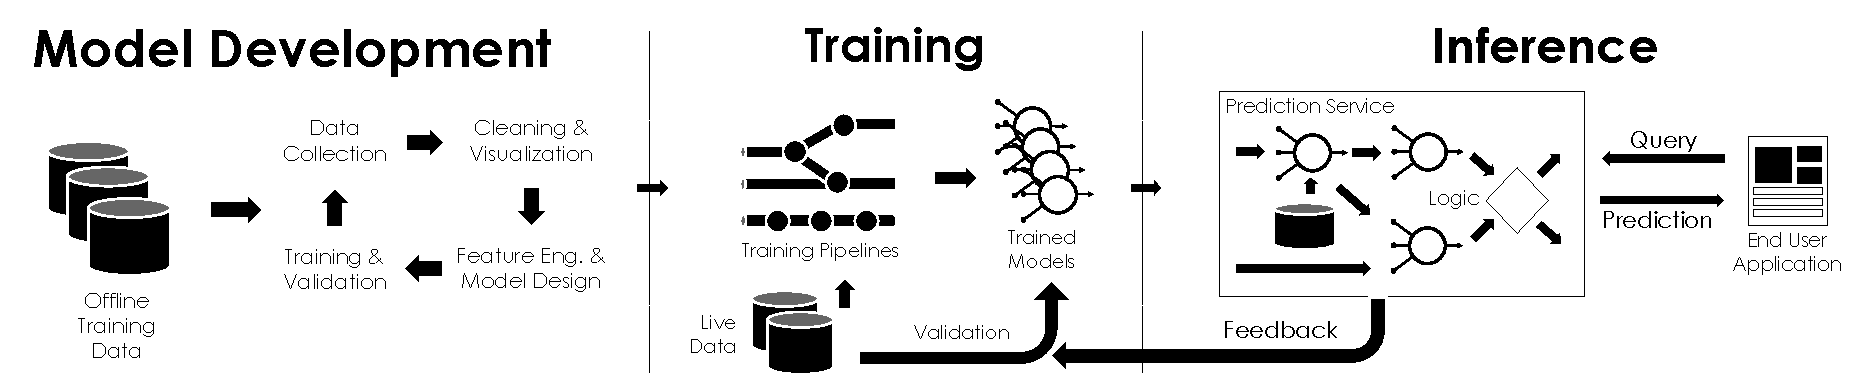
\includegraphics[width=\textwidth]{letters/pipeline.pdf}
\caption{\small \textbf{Machine Learning Life-cycle.} A simplified depiction of the key stages of a machine learning application.}
\label{fig:mllc}
\end{figure}


The machine learning life-cycle (Fig.~\ref{fig:mllc}) spans not only the model development but also production training and inference.
Each stage demands different skills (e.g., neural network design, data management, and cluster management) and imposes different requirements on the underlying systems.
Yet there is an overwhelming need for unifying design principles and technologies to address pervasive problems including feature management, data provenance, pipeline reproducibility, low-latency serving, and prediction monitoring just to name a few.


There has been a flurry of recent progress in systems to aid in managing the machine learning life-cycle.  
Large industrial projects like 
FB Learner Flow 
% \href{https://code.fb.com/core-data/introducing-fblearner-flow-facebook-s-ai-backbone/}{FB Learner Flow}
from Facebook, 
Michelangelo 
% \href{https://eng.uber.com/michelangelo/}{Michelangelo} 
from Uber, and 
TFX 
% \href{https://www.tensorflow.org/tfx/}{TFX} 
from Google have received considerable recent attention.  
In this issue, we have solicited papers from several recent industrial and academic projects that have received slightly less attention.


The first paper provides an overview of several real-world use cases and then outlines the key conceptual, data management, and engineering challenges faced in production machine learning systems.
% Rather than advocating a single system, this work describes some design principles that can inform potential solutions.
The second and third papers explores the challenges of model management and provenance across the machine learning life-cycle.
They motivate the need for systems to track models and their meta-data to improve reproducibility, collaboration, and governance. 
% expands upon the machine learning life-cycle 
% to include: data preparation, feature engineering, model training, deployment, and maintenance
% and explores the challenges of model 
The second paper introduces, ModelDB, an open-source system for model management and describe some of the functionality and design decisions. 
The third paper describes a related system, ProvDB, that uses a graph data model to capture and query fine-grained versioned lineage of data, scripts, and artifacts throughout the data analysis process.
The fourth paper describes, MLFlow, a new open-source system to address the challenges of experimentation, reproducibility, and deployment. 
This work leverages containerization to capture the model development environment and a simple tracking API to enable experiment tracking.
% The extensible model containerization enables model developers to more easily collaborate around modeling environments and then deploy model containers.
The fifth paper focuses on inference and explores the challenges and opportunities of serving white-box prediction pipelines.  
Finally, we solicited a summary of the recent Common Modeling Infrastructure (CMI) workshop at KDD 2018, which provides a summary of the keynotes and contributed talks.

The work covered here is only a small sample of the emerging space of machine learning life-cycle management systems. 
We anticipate that this will be a growing area of interest for the data engineering community.


% In contrast to the containerization of pipelines in MLFlow, the Microsoft team leverage knowledge about the internal of the prediction pipeline to more efficient serve predictions. 



\end{document}



%\end{news}


%\end{newssection}

%\begin{newssection}{TCDE Election}

% there will be other letters- and a blank page will appear in your document
% but the special issue part will be fine

%\begin{news}{Letter from the Editor-in-Chief}
%{David Lomet}{Microsoft Corporation}
%\documentclass[11pt]{article} 

\usepackage{deauthor,times,graphicx}
%\usepackage{url}
\usepackage{hyperref}

\begin{document}

\subsection*{ICDE 2018}

Repeating my comment from the last issue-

The IEEE International Conference on Data Engineering will be held in April 14-19, 2018 in Paris, France.  This is the flagship conference of the Computer Society's Technical Committee on Data Engineering.  It is a great conference, at a great location.  What could possibly be better than April in Paris at ICDE!  I am attending and hope to see you there.

\subsection*{About the Bulletin}

This March current issue marks the end of editorial tenure for the Bulletin's current set of editors.  So it is once again time for me to pat myself on the back.  This current set, Tim Kraska, Tova Milo, and Haixun Wang, continue my outstanding success (he says modestly) in finding and choosing great editors.  All three have done truly fine jobs at producing issues that bring to our readers surveys of the latest work in very current areas. The success of the Bulletin depends on great issue editors.  I want to thank Tim, Tova, and Haixun for being exactly that with the fine jobs that they have done.  There was unexpected ``scrambling" over the past two years, so I want to thank them also for their flexibility in coping with this.  


\subsection*{The Current Issue}

Don't you get tired of someone shouting ``FAKE NEWS!".  Or perhaps even worse, being exposed to fake news before it has been labeled as such?  Our political conversations seem increasingly to include many variations of ``fake news" and discussions about which news is fake.  ``Sad." So where am I going with this?

The database world has been working on a key aspect of this problem for many years.  The technical area is called ``data provenance".  And it addresses the problem of where information comes from and how it impacts the subsequent processing of data and the reported results.  The June, 2010 issue was the last one on provenance.  And seven years is a long time in an active technical area, especially an area as important as this.

The current issue is focused on the applications of provenance.  Without delving into the current political scene, a reader will clearly see how extensively provenance management can be used.  As we gain more insight into its application scenarios, we also gain more insight into how to manage provenance.  This symbiotic relationship is driving the field forward.   Tova Milo, our Bulletin editor for the issue, has done an excellent job in bringing the issue together, making it a great place to learn about and track progress in the field.  The result is an issue well worth reading.



\end{document}



%\end{news}
%
%\newpage
%
%% your introductory letter goes here
%
%\begin{news}{Letter from the Special Issue Editor}
%{Joseph E. Gonzalez}{University of California at Berkeley\\ Berkeley, CA}
%\documentclass[11pt]{article} 

\usepackage{deauthor,times,graphicx}
%\usepackage{url}
\usepackage{hyperref}



\begin{document}

Machine learning is rapidly maturing into an engineering discipline at the center of a growing range of applications.
This widespread adoption of machine learning techniques presents new challenges around the management of the data, code, models, and their relationship throughout the machine learning life-cycle.
In this special issue, 
% of the Data Engineering Bulletin 
we have solicited work from both academic and industrial leaders 
% in the data engineering community that 
who are exploring how data engineering techniques can be used to address the challenges of the machine learning life-cycle.




\begin{figure}[h]
\centering
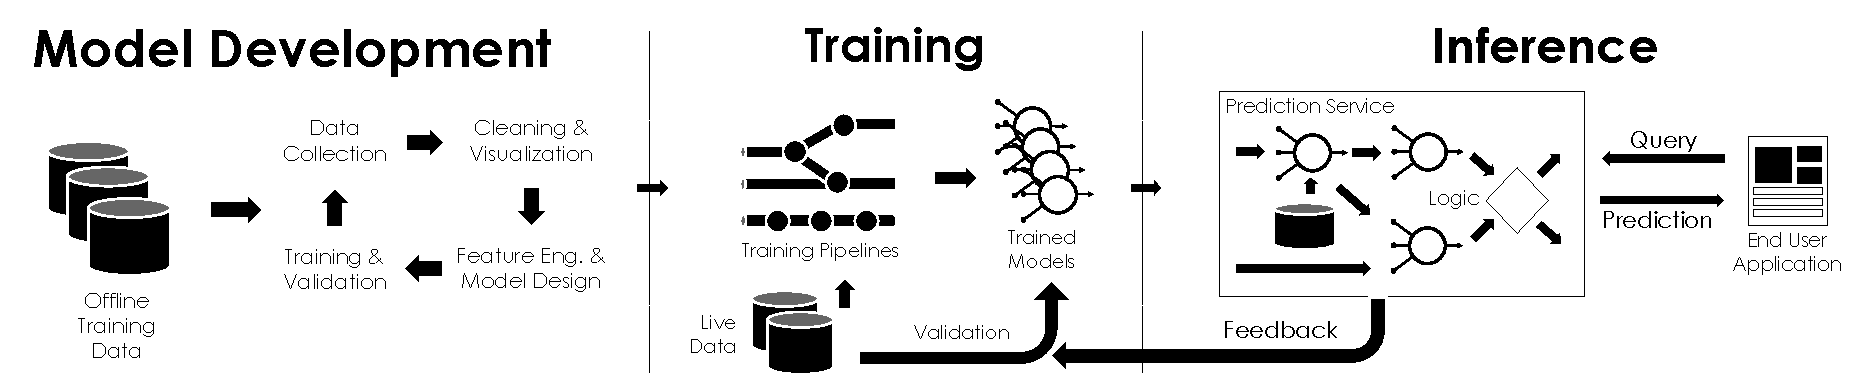
\includegraphics[width=\textwidth]{letters/pipeline.pdf}
\caption{\small \textbf{Machine Learning Life-cycle.} A simplified depiction of the key stages of a machine learning application.}
\label{fig:mllc}
\end{figure}


The machine learning life-cycle (Fig.~\ref{fig:mllc}) spans not only the model development but also production training and inference.
Each stage demands different skills (e.g., neural network design, data management, and cluster management) and imposes different requirements on the underlying systems.
Yet there is an overwhelming need for unifying design principles and technologies to address pervasive problems including feature management, data provenance, pipeline reproducibility, low-latency serving, and prediction monitoring just to name a few.


There has been a flurry of recent progress in systems to aid in managing the machine learning life-cycle.  
Large industrial projects like 
FB Learner Flow 
% \href{https://code.fb.com/core-data/introducing-fblearner-flow-facebook-s-ai-backbone/}{FB Learner Flow}
from Facebook, 
Michelangelo 
% \href{https://eng.uber.com/michelangelo/}{Michelangelo} 
from Uber, and 
TFX 
% \href{https://www.tensorflow.org/tfx/}{TFX} 
from Google have received considerable recent attention.  
In this issue, we have solicited papers from several recent industrial and academic projects that have received slightly less attention.


The first paper provides an overview of several real-world use cases and then outlines the key conceptual, data management, and engineering challenges faced in production machine learning systems.
% Rather than advocating a single system, this work describes some design principles that can inform potential solutions.
The second and third papers explores the challenges of model management and provenance across the machine learning life-cycle.
They motivate the need for systems to track models and their meta-data to improve reproducibility, collaboration, and governance. 
% expands upon the machine learning life-cycle 
% to include: data preparation, feature engineering, model training, deployment, and maintenance
% and explores the challenges of model 
The second paper introduces, ModelDB, an open-source system for model management and describe some of the functionality and design decisions. 
The third paper describes a related system, ProvDB, that uses a graph data model to capture and query fine-grained versioned lineage of data, scripts, and artifacts throughout the data analysis process.
The fourth paper describes, MLFlow, a new open-source system to address the challenges of experimentation, reproducibility, and deployment. 
This work leverages containerization to capture the model development environment and a simple tracking API to enable experiment tracking.
% The extensible model containerization enables model developers to more easily collaborate around modeling environments and then deploy model containers.
The fifth paper focuses on inference and explores the challenges and opportunities of serving white-box prediction pipelines.  
Finally, we solicited a summary of the recent Common Modeling Infrastructure (CMI) workshop at KDD 2018, which provides a summary of the keynotes and contributed talks.

The work covered here is only a small sample of the emerging space of machine learning life-cycle management systems. 
We anticipate that this will be a growing area of interest for the data engineering community.


% In contrast to the containerization of pipelines in MLFlow, the Microsoft team leverage knowledge about the internal of the prediction pipeline to more efficient serve predictions. 



\end{document}



%\end{news}

%\end{newssection}



\begin{callsection}
%  This section will be empty for your version
%
%  Calls for papers section.  Use the callsection environment.
%  Each call for papers is contained in an call environment, where the single 
%  required options to \begin{call} is the name of the conference.
%
\begin{call}{ICDE 2019 Conference}
\centerline{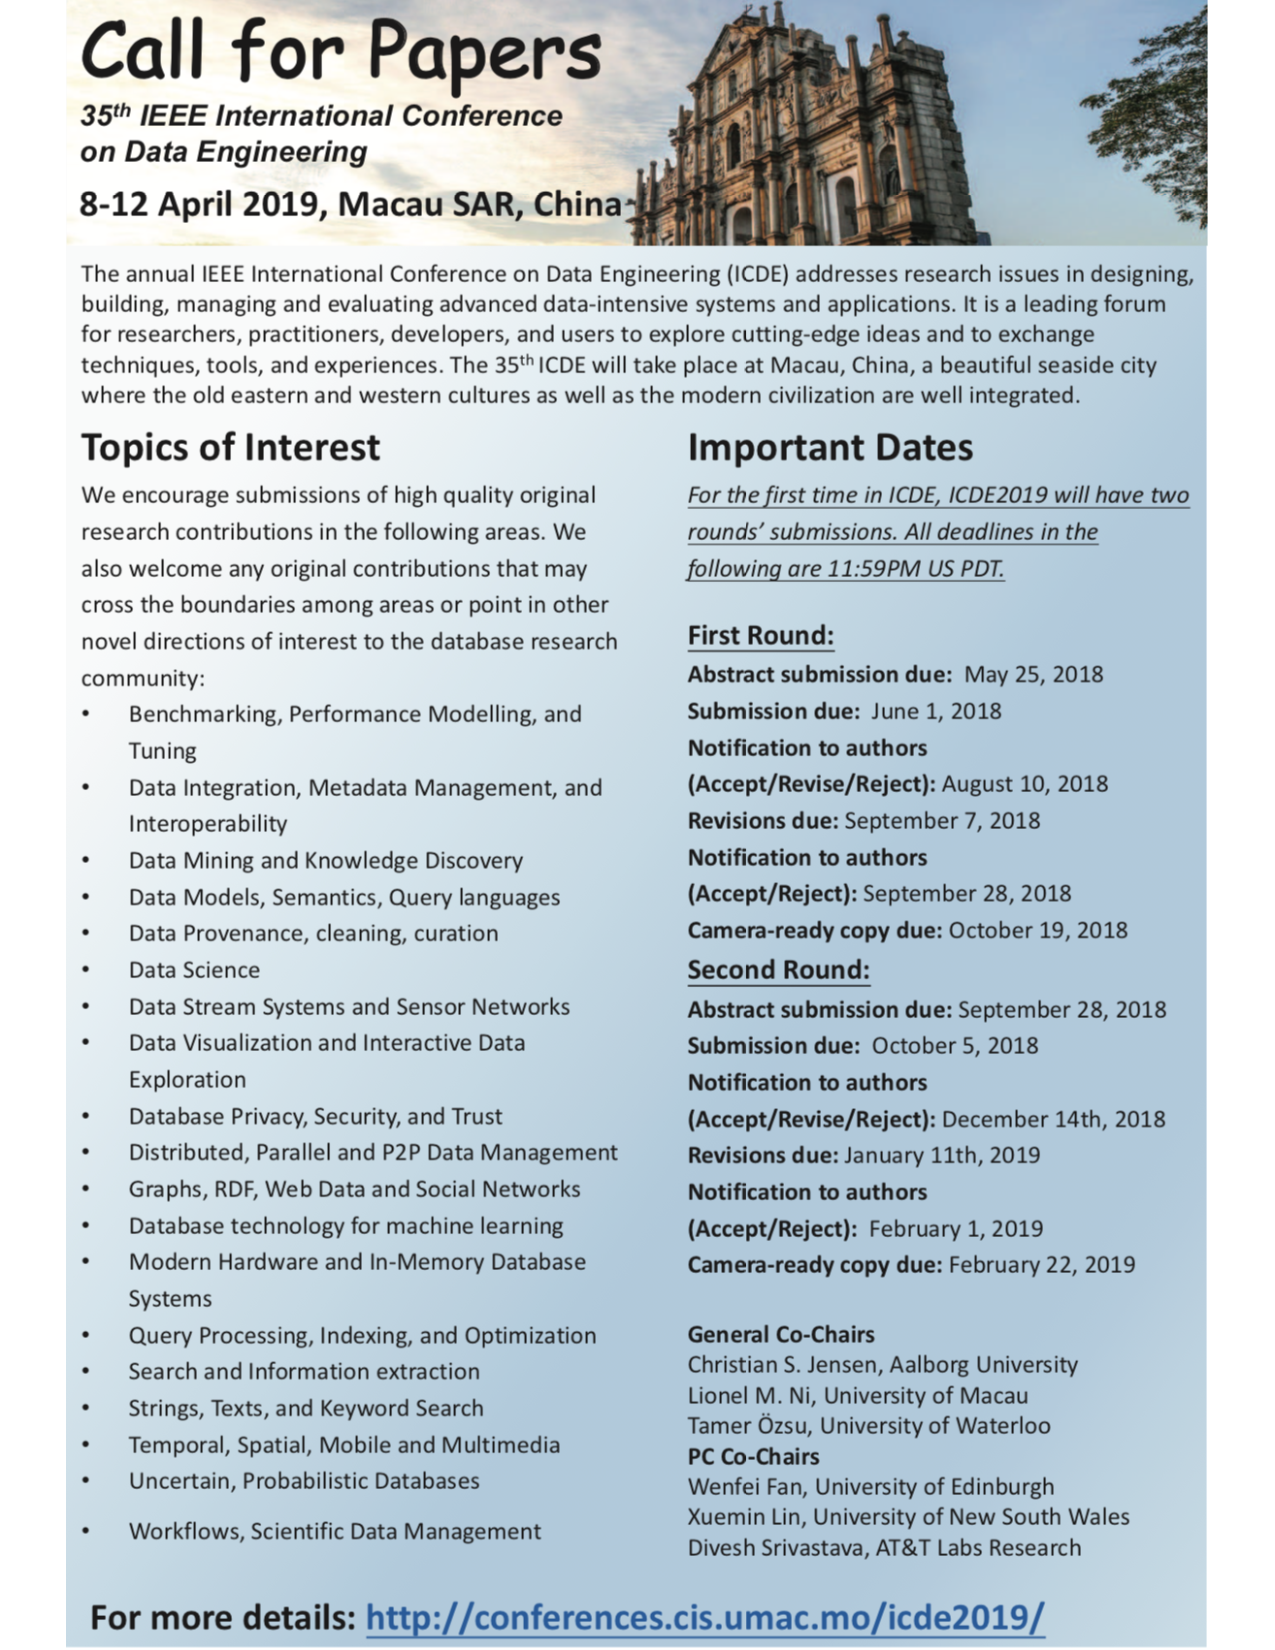
\includegraphics[width=\textwidth, bb= 0 0 610 790] {calls/icde19.pdf}} 
%\centerline{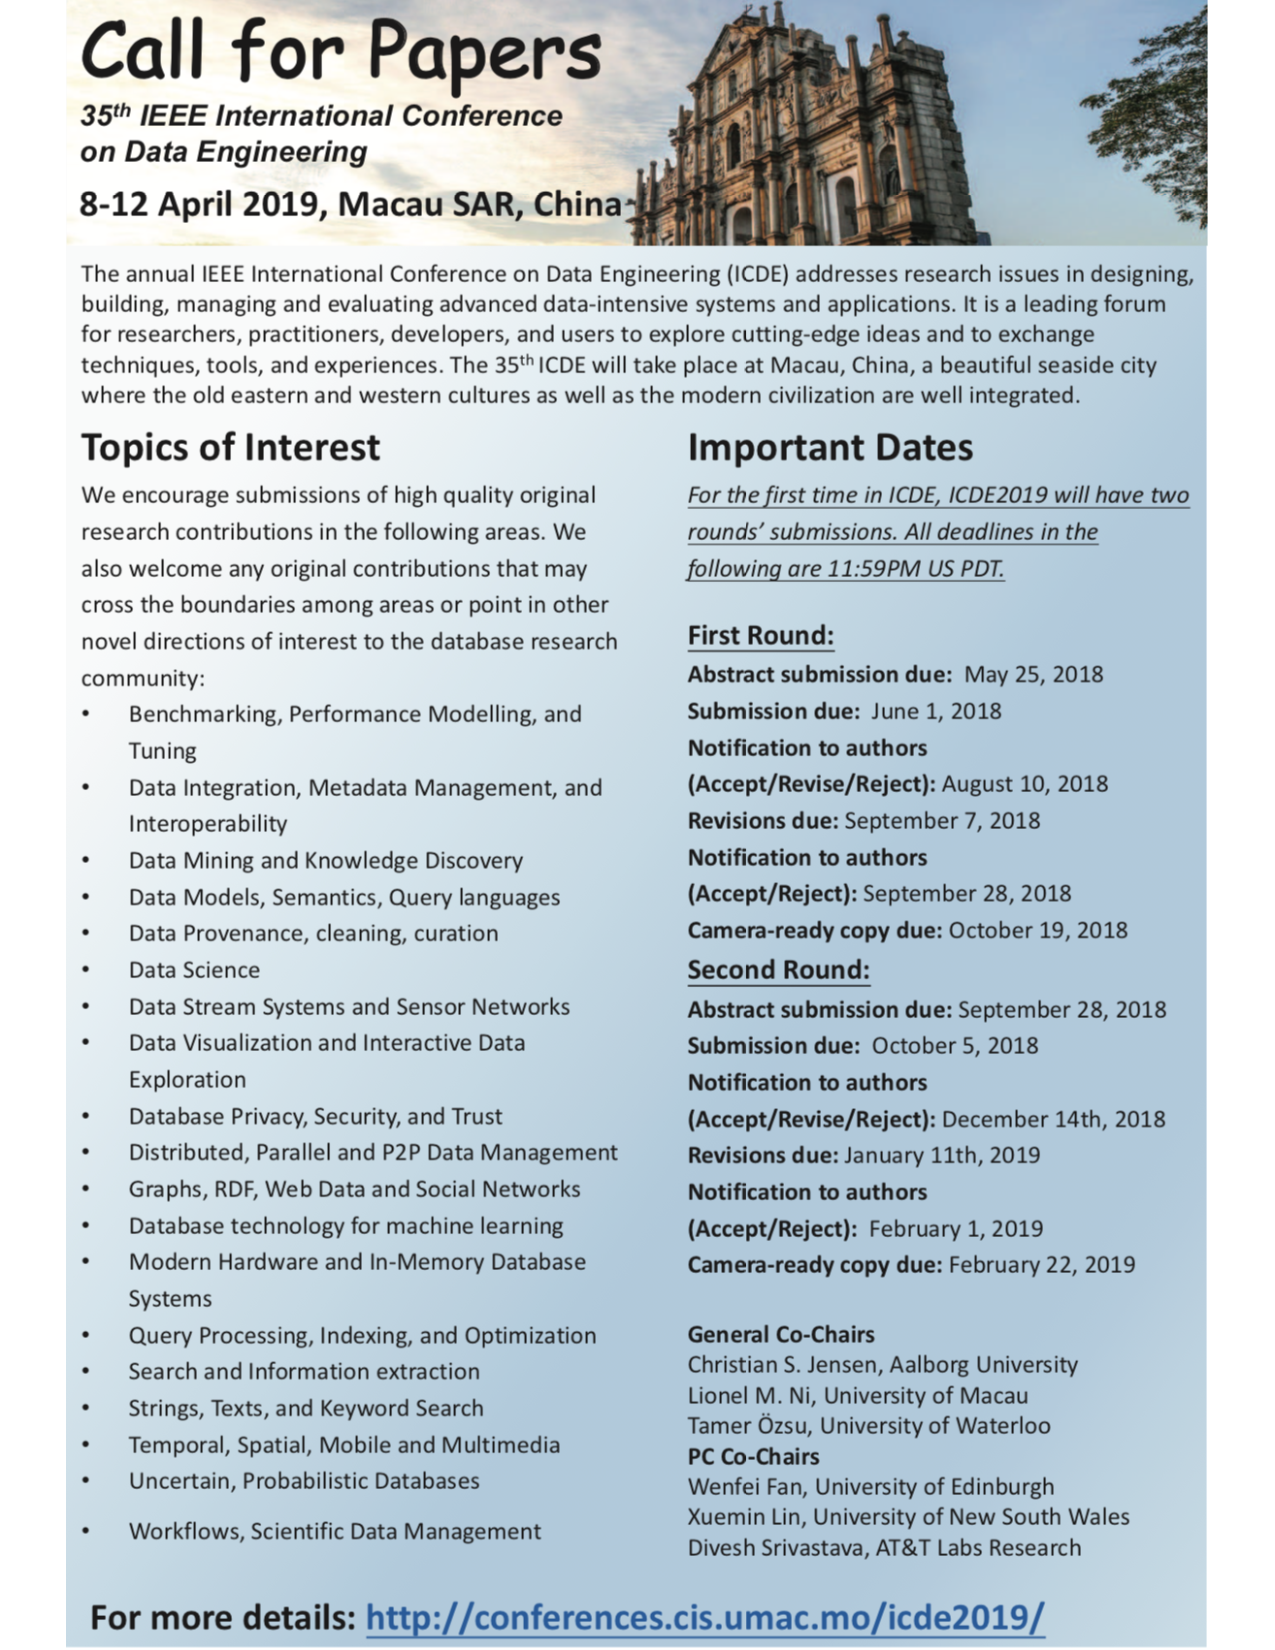
\includegraphics[width=\textwidth, bb= 0 0 590 760] {calls/icde19.pdf}}
\end{call}
\begin{call}{TCDE Membership Form}
%\centerline{\includegraphics[width=\textwidth, bb= 0 0 610 790]
\centerline{
\includegraphics[width=\textwidth, bb= 0 0 590 760] {calls/tcde.pdf}}
\end{call}
\end{callsection}

\end{bulletin}
\end{document}
